\chapter{Солнечный блик как ``инструмент'' исследования Океана из Космоса} \label{chap:1}

Морозным днем 31 декабря 2008 года я плыл на пароме по Севастопольской бухте и уже в который раз наблюдал всем хорошо известное явление~--~солнечный блик (см. Рисунок~\ref{fig:1}). Те, кто живут у моря, настолько привыкли наблюдать блики на морской поверхности, что их это давно не удивляет. Те же, кто приехал отдохнуть, нежатся под лучами солнца и прикрываются солнцезащитными очками, чтобы бликующая поверхность не слепила глаза. И лишь некоторые вспоминают о бликах, когда играют с детьми или со своими питомцами, ``пуская солнечных зайчиков``, отраженных от зеркала пудреницы. Но, несмотря на то, что явление это, казалось бы, довольно обыденное, оно далеко не полностью изучено и, уверен, о применении его будет написана ещё ни одна диссертация. 



\section{Общие представления} \label{sec:1.1}


Спутниковое дистанционное зондирование (ДЗ)~--~это регистрация датчиком, установленным на искусственном спутнике, электромагнитного излучения, которое отражается или испускается поверхностью Земли~\citep{Robinson2004}. При дистанционном зондировании океанов, морей и др. водных объектов одним из источников измеряемого излучения является солнечный свет, который проникает в толщу воды, частично поглощается ею, а также рассеивается и отражается, в том числе и в направлении удалённого датчика (см. Рисунок~\ref{fig:2}).



\begin{figure}[!thb]
 \center
 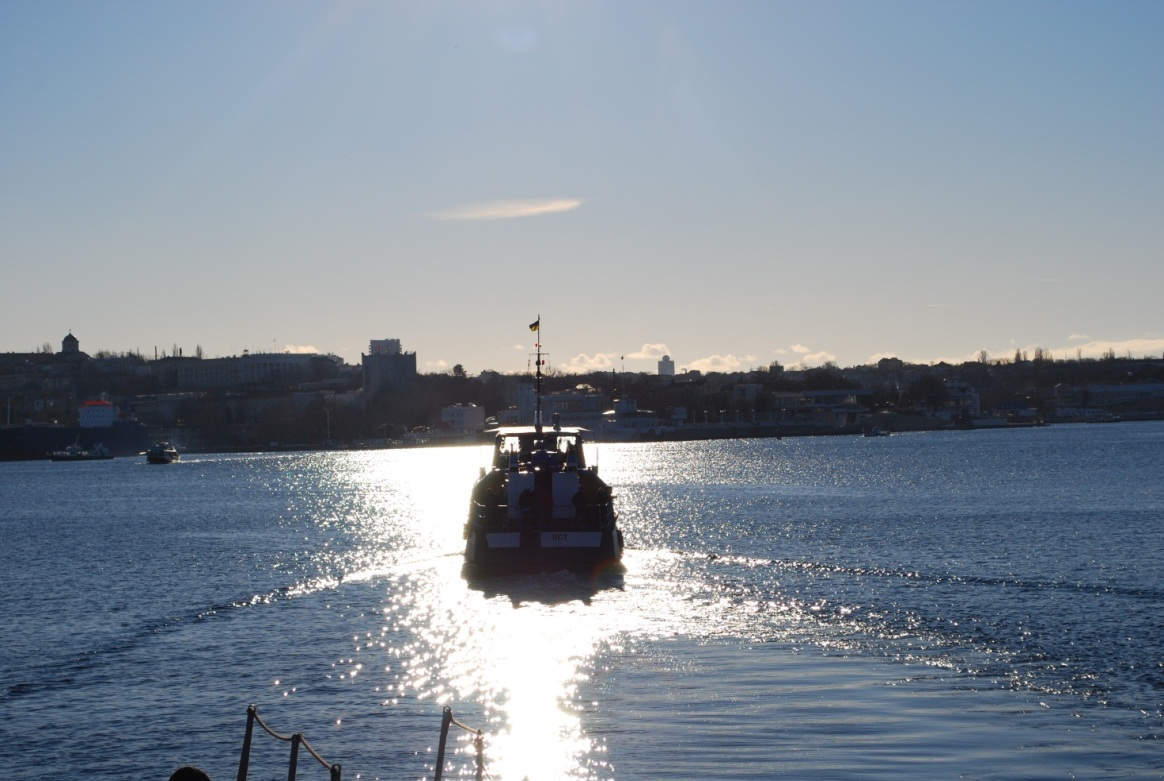
\includegraphics[width=\linewidth]{fig1}
 \floattitle{Солнечный блик в середине дня должен был быть виден как симметричное яркое пятно, но ветер, течения, слики и проходящие суда сформировали на морской поверхности множество уклонов, благодаря которым мы наблюдаем сложную картину зеркальных отражений~--~множество ``солнечных зайчиков``, которые, сливаясь воедино, формируют неподражаемую картину}
 \caption{Солнечный блик в Севастопольской бухте, 31 декабря 2008г.}
 \label{fig:1}
\end{figure}

Фотоны, попадающие в водную среду, взаимодействуют с молекулами воды, органическим веществом, растворенным в воде, клетками микроводорослей, взвешенными веществами (такими как минеральная взвесь, детрит) и планктонными организмами (такими как бактерио-- и зоопланктон).



\begin{figure}[!thb]
 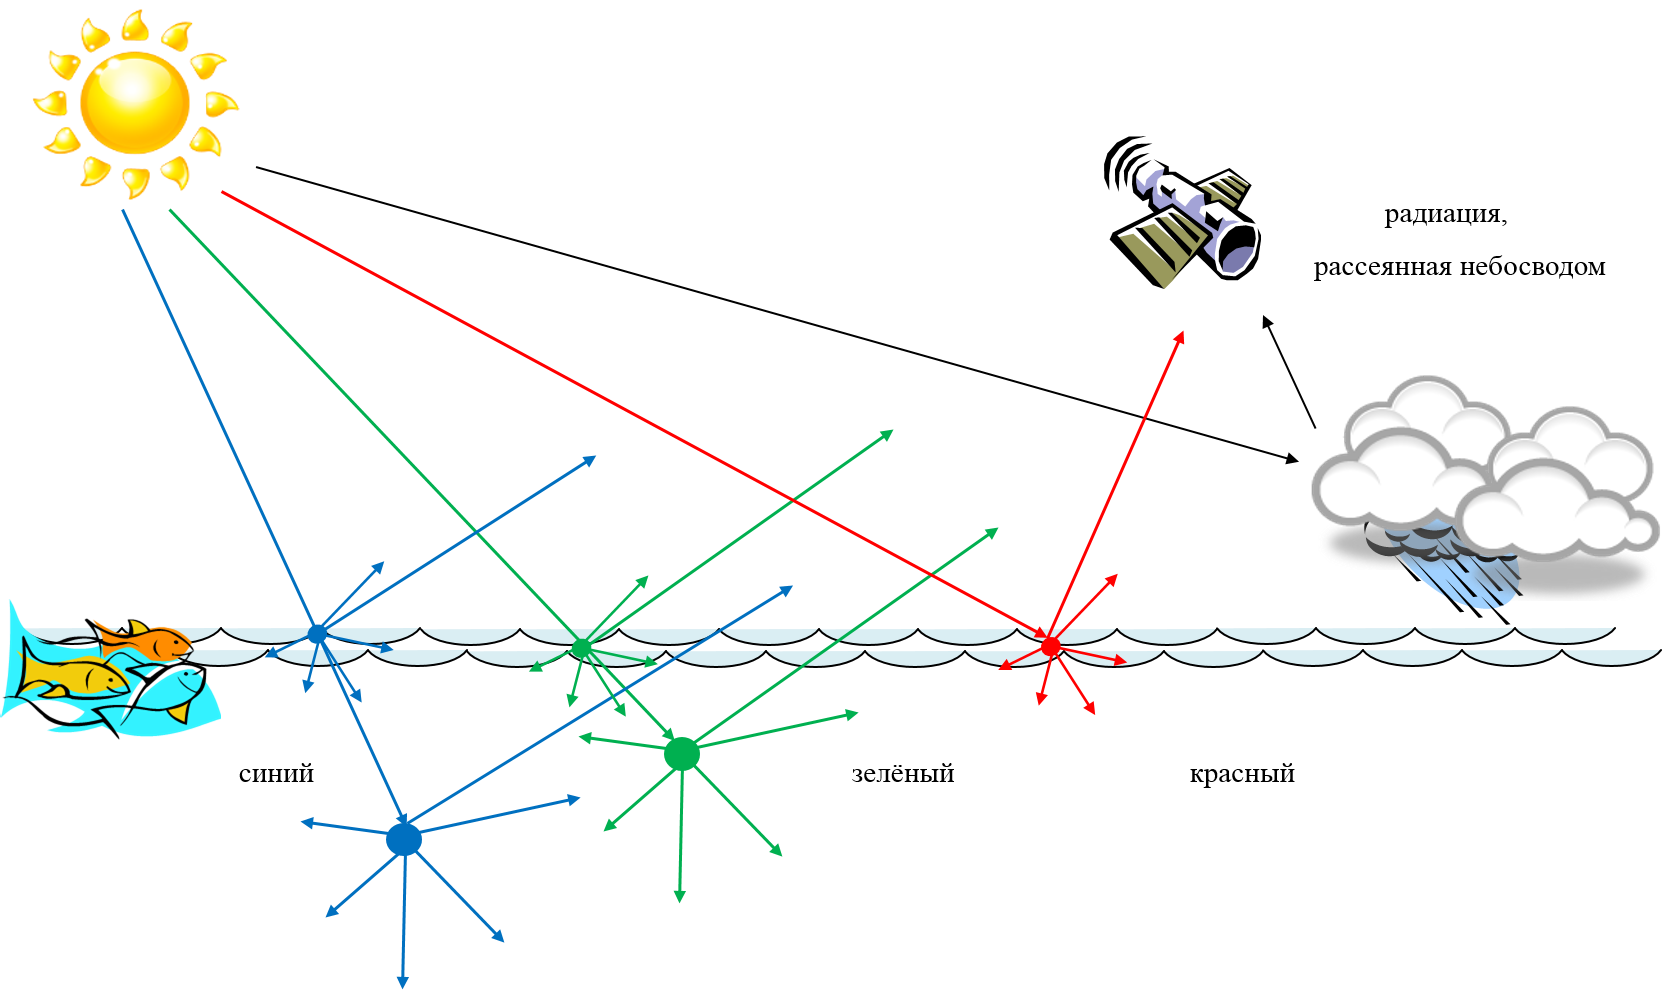
\includegraphics[width=\linewidth]{fig2}
 \floattitle{Солнечный свет проникает в толщу воды, частично поглощается ею, а также рассеивается и отражается, в том числе и в направлении дистанционного датчика. Обратим внимание, что свет в красном канале поглощается в ``тонком'' поверхностном слое Океана~\citep{Jerlov1976}, и, таким образом, не так чувствителен к ``цвету'' водного столба, а также не чувствителен к поверхностной температуре}
 \caption{Схематическое изображение компонент солнечного излучения регистрируемого спутниковым датчиком}
 \label{fig:2} 
\end{figure}

Большая часть солнечной энергии поглощается водой и превращается в тепло, но часть фотонов оказывается рассеянной, в том числе, и в направлении раздела вода-воздух. В результате фотон может покинуть водную среду и достигнуть удаленного датчика. Величина вероятности рассеяния зависит как от размера рассеивающего компонента и его комплексного показателя преломления, так и от энергии фотона. Спектральное распределение света, вышедшего из воды, зависит от положения Солнца, состояния облачности и природных свойств самой воды и веществ, в ней находящихся.

Восприятие цвета воды человеческим глазом определяется спектральным распределением света, восходящего из-под поверхности воды. Так чистые океанические воды имеют голубой цвет, а прибрежные воды могут быть зеленоватыми, бурыми или желтоватыми в зависимости от наличия в воде микроводорослей, неорганических взвесей и растворенных органических веществ~\citep{Pozdnyakov2003}.

Вышеизложенный принцип рассеяния радиации в верхнем слое Океана лежит в основе спутниковых оптических методов исследования оптических свойств воды (концентрации хлорофилла, взвешенного вещества и т.д.). Однако в области солнечного блика значительная часть попадающего в приёмник излучения является отражённой от поверхности солнечной радиацией, энергия которой значительно превышает восходящую из толщи морской воды. В этом случае исследования оптических свойств воды невозможны. Как будет показано ниже, излучение, отражённое от морской поверхности содержит очень ценные сведения о шероховатости морской поверхности, которая, в свою очередь, несёт информацию о процессах, протекающих в верхнем слое Океана. Следовательно, исследования солнечного блика могут рассматриваться как потенциально важный и эффективный метод диагностирования Океана из Космоса.



\newpage

\section{Оптические исследования Океана из Космоса} \label{sec:1.2}


Оптические методы~--~традиционные и широко используемые спутниковые методы исследования Океана. Некоторые характеристики наиболее часто используемых оптических спектрометров приводятся в Таблице~\ref{tab:1}. В работе использованы данные дистанционного зондирования, полученные в оптическом диапазоне двумя спектрометрами MODIS и MERIS (Таблицы~\ref{tab:1},~\ref{tab:2}). В значительной мере специализированные под задачи дистанционного зондирования Мирового Океана, эти приборы установлены на искусственных спутниках Земли, летающих на околополярной орбите. Это обеспечивает возможность получать ежедневные данные по всей поверхности Земли. Работа спутников обеспечивается наземными службами, которые получают исходные данные со спутника по радиоканалу, проводят их первичную обработку и распространяют готовые данные зондирования через Интернет или адресно рассылают их на CD потребителям.

Одно из основных применений данных, полученных с помощью спутниковых оптических сканеров,~--~изучение оптических характеристик верхнего слоя Океана (цвет океанической воды, содержание фитопланктона и минеральной взвеси, биогеохимические характеристики), а также температуры его поверхности (см., например, \citep{Doerffer2007,Korosov2009}).



\begin{table}
 \centering
 \begin{tabular}{|p{1.2in}|p{0.7in}|p{0.9in}|p{0.8in}|p{0.7in}|} \hline 
 Датчик & SeaWiFS & MODIS & MERIS & AVHRR \\ \hline 
 Спутник & SeaStar & Aqua, Terra & ENVISAT & NOAA \\ \hline 
 Год запуска & 1997 & 2000, 2001 & 2002 & 1987 \\ \hline 
 Полоса обзора, км & 2800 & 2300 & 1150 & 2580 \\ \hline 
 Среднее спектральное разрешение, нм & 20 & 10 & 10 & 500 \\ \hline 
 Спектральный диапазон, нм & 412~--~865 & 405~--~14385 & 390~--~1040 & 590~--~12000 \\ \hline 
 Количество каналов & 8 & 36 & 15 & 5 \\ \hline 
 Пространственное разрешение в надире, км & 1.1 & 0.25\newline 0.5\newline 1.1 & 0.3\newline 1.2 & 1.1 \\ \hline
 \end{tabular}
 \caption{Основные характеристики некоторых спутниковых спектрометров}
 \label{tab:1}
\end{table}



\begin{table}
 \centering
 \begin{tabular}{|p{0.7in}|p{1.0in}|p{1.0in}|p{0.7in}|p{1.0in}|} \hline 
 Номера каналов & Спектральный диапазон (мкм) & Пространств. разрешение (м) & Полоса обзора (км) & Повторяемость съемки одной территории \\ \hline 
 1-2 & 0.62 - 0.88 & 250 & 2300 & 1-2 раза в сутки, в зависимости от широты места съемки \\ \hline 
 3-7 & 0.46 - 2.16 & 500 & 2300 & \\ \hline 
 8-19 & 0.41 - 0.97 & 1000 & 2300 & \\ \hline 
 20-25 & 3.66 - 4.55 & 1000 & 2300 & \\ \hline 
 26 & 1.36 - 1.39 & 1000 & 2300 & \\ \hline 
 27-36 & 6.54 - 14.39 & 1000 & 2300 & \\ \hline 
 \end{tabular}
 \caption{Основные характеристики спектрометра MODIS}
 \label{tab:2}
\end{table}

В этом случае солнечная радиация, отраженная от морской поверхности, является шумом по отношению к радиации рассеянной в верхнем слое Океана. В областях солнечного блика отражённая радиация составляет значительную часть регистрируемого излучения, что, в свою очередь, порождает большие трудности при создании алгоритмов восстановления ``цвета'' Океана. Так, например, для маскирования пикселей изображений MERIS морской поверхности, содержащих яркости солнечного блика, создан специальный алгоритм, включённый в стандартные алгоритмы атмосферной коррекции продуктов MERIS~\citep{Montagner2003}.

На Рисунке~\ref{fig:3a} приводится пример ``глобальной'' маски блика от 21 марта 2004 года для MODIS/Aqua, а на Рисунке~\ref{fig:3b} для SeaWiFS. Из приведённых примеров видно, что огромная часть объёма данных на значительных акваториях не может быть использована, маскируется для конечного пользователя и, таким образом, ``выбрасывается в мусорный ящик``.

Основной целью работы является разработка методов и алгоритмов, дающих возможность использовать данные о яркости океанической поверхности внутри солнечного блика, для исследования океанографических явлений по их поверхностным проявлениям.



\subsection{Солнечный блик как источник информации о поверхностных явлениях}


Как было отмечено, основные океанографические приложения оптических спутниковых данных связаны с изучением цвета Океана. С одной стороны, отражённый от морской поверхности солнечный свет составляет основной вклад восходящей радиации и создаёт значительные трудности для разработчиков алгоритмов восстановления цвета Океана. Однако, в солнечном блике содержится ценная информация о статистических характеристиках шероховатости морской поверхности, её среднеквадратичном наклоне (СКН), асимметрии и эксцессе, как было впервые показано в работе Кокса и Манка~\citep{Cox1954, Cox1954a}, а также Бреоном и Хенриотом~\citep{Breon2006}.



\begin{figure}[!thb]
	\centering
    \subcaptionbox{\label{fig:3a}}
    {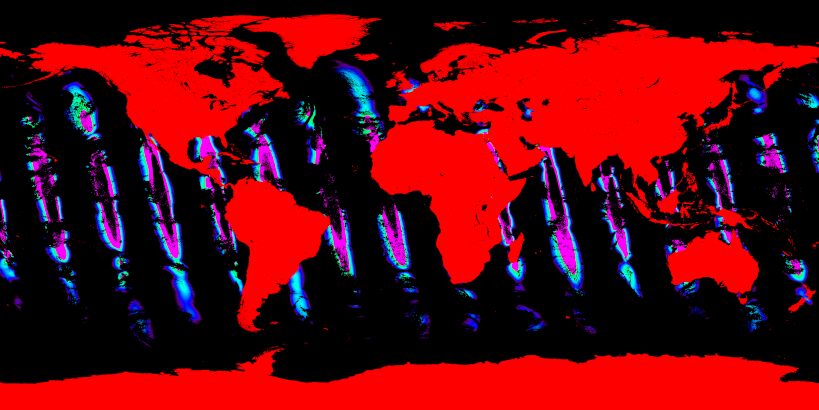
\includegraphics[width=0.49\linewidth]{fig3a}}
    \subcaptionbox{\label{fig:3b}}
    {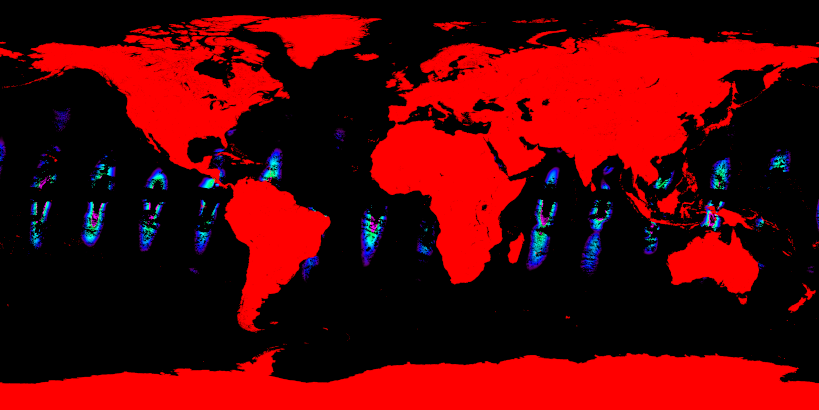
\includegraphics[width=0.49\linewidth]{fig3b}}
    \\
    \floattitle{Внушительная часть данных оптического диапазона на значительных акваториях не может быть использована и потому маскируется}
    \caption{``Глобальная'' маска блика от 21 Марта 2004 года для MODIS/Aqua и SeaWiFS}
    \label{fig:3}
\end{figure}

Большинство явлений на поверхности Океана, как, например, биогенные и нефтяные плёнки, внутренние волны (ВВ), кильватерные струи за судном, спиралевидные вихри, оказывают локальное влияние на шероховатость поверхности, что и приводит к их проявлениям в оптических данных. Существует много работ, посвящённых спутниковым наблюдениям поверхностных сликов в солнечном блике, например~\citep{Adamo2005, Chust2007, Hu2009}. Хеннингс и др.~\citep{Hennings1994} представили результаты наблюдений поверхностных проявлений рельефа дна на мелководье по спутниковым изображениям солнечного блика. Авторы работ~\citep{Apel1975, Artale1990, Mitnik2000} наблюдали и изучали проявления нелинейных ВВ в солнечном блике. Джэксон и Алперс~\citep{Jackson2010} использовали данные прибора MODIS в солнечном блике для определения пространственного распределения ВВ по всемирному Океану.

Очевидно, что контрасты яркости в солнечном блике вызваны пространственными вариациями ``шероховатости'' морской поверхности, вследствие воздействия океанических процессов на ветровые волны. В случае с поверхностными сликами, амплитуда наблюдаемых контрастов связана с типом плёнки (биогенного происхождения или нефти), а также, вероятно, с толщиной нефтяной плёнки, образующей слик. Таким образом, количественная интерпретация контрастов яркости в солнечном блике может существенно приблизить нас к лучшему пониманию механизмов подавления коротких волн.

На данный момент существует несколько исследований, посвящённых проблеме восстановления аномалий шероховатости по изображениям солнечного блика. Бурдюгов с соавторами~\citep{Burdyugov1987} использовали модель Кокса и Манка~\citep{Cox1954} для восстановления контрастов СКН по вариациям яркости в солнечном блике, применив этот подход к аэрофотографиям поверхностных сликов, образованных прохождением серий ВВ. Также ранее был предложен метод восстановления двумерного спектра возвышений поверхностных волн по изображениям солнечного блика (см., например,~\citep{Stilwell1969, Bolshakov1990}). В работе ~\citep{Bolshakov1990a} эти данные использовались для исследования эволюции и трансформации двумерного спектра ветрового волнения.

Насколько известно, в отличие от определения ``фоновых'' статистических свойств уклонов морской поверхности, спутниковые изображения солнечного блика никогда ранее не использовались для количественных оценок аномалий СКН шероховатости морской поверхности. Поскольку яркость в солнечном блике, как и её контрасты, вызванные теми или иными явлениями, зависят от геометрии наблюдения и положения Солнца, возникают определённые трудности с интерпретацией. Так контрасты СКН могут проявляться как в виде тёмных, так и ярких аномалий яркости (см., например,~\citep{Hu2009} для нефтяных сликов;~\citep{Matthews2005, Munk1987} для кильватерных струй и ВВ;~\citep{Munk2000} для вихрей;~\citep{Jackson2010} для ВВ и нефтяных загрязнений). Это свойство следует непосредственно из геометрии наблюдения, когда зеркальные точки располагаются по разные стороны зон инверсии контрастов, как показано в работах~\citep{Burdyugov1987} и~\citep{Jackson2010}.



\newpage

\section{Модель изображения морской поверхности в области солнечного блика} \label{sec:1.3}


При условии, что океан мог бы оказаться совершенно спокойным, а его поверхность невозмущённой, то на поверхности сформировался бы единственный солнечный блик с центром в зеркальной точке. Однако, в природе мы часто наблюдаем другую картину, когда множество ``солнечных зайчиков'' формируют сложную ``бликующую'' картину на взволнованной водной глади.

В этом случае, излучение, приходящее в приёмник, формируется совокупностью зеркальных отражений от склонов поверхностных волн, распределённых по морской поверхности.

Для исследования солнечного блика наиболее предпочтителен красный канал, поскольку свет в красном канале поглощается в ``тонком'' поверхностном слое Океана~\citep{Jerlov1976}, и, таким образом, менее чувствителен к ``цвету'' водного столба, а также не чувствителен к поверхностной температуре.

Солнечный блик несёт в себе очень ценную информацию о статистических характеристиках морской поверхности~--~среднеквадратичном наклоне (СКН), асимметрии и кривизне, что было отчётливо показано в пионерских работах Кокса и Манка~\citep{Cox1954, Cox1954a, Cox1956}, а также описано в недавней работе~\citep{Breon2006}, в которой авторы использовали огромный массив спутниковых данных оптического диапазона. Поскольку количество отражённой радиации в районе солнечного блика зависит от СКН, любое явление, наблюдаемое на поверхности Океана (как слики, внутренние волны, фронты течений, вихри, грибовидные структуры и др.), приводящее к вариациям СКН, возможно наблюдать в контрастах яркости.



\subsection{Основные соотношения}


Геометрия зеркального отражения солнечного излучения от уклонов взволнованной поверхности Океана приведена на Рисунке~\ref{fig:4}. Зеркальные отражения должны удовлетворять двум условиям:
\begin{itemize}
	\item угол падения равен углу отражения;
	\item луч падающий ($I$), луч отражённый ($R$) и перпендикуляр ($n$) к отражающей поверхности в точке излома луча всегда лежат в одной плоскости
\end{itemize}



\begin{equation} \label{eq:1.1} 
    \left[\left(\vec{R}-\vec{I}\right)\times \vec{n}\right]=0 \mbox{ или } \left(\vec{R}-\vec{I}\right)=2\vec{n}\cos \omega
\end{equation}


\begin{figure}[!thb]
    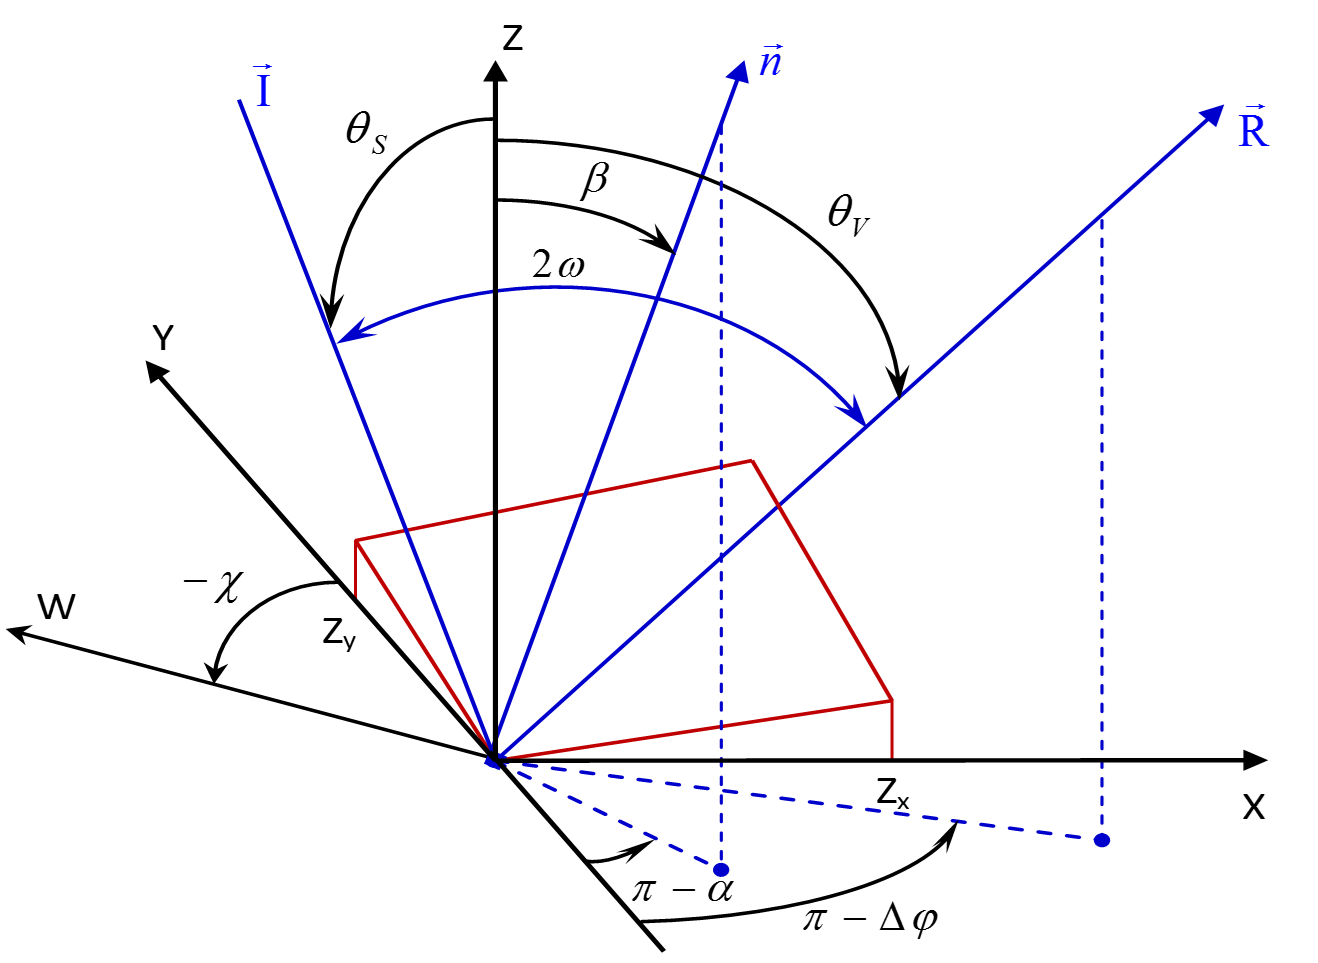
\includegraphics[width=\linewidth]{fig4}
    \floattitle{Система координат выбрана таким образом, что ось y сонаправлена с азимутом Солнца, $\theta _{s} ,\, \theta _{V} $~--~зенитные углы Солнца и сенсора, соответственно, $\varphi _{V} $~--~азимут сенсора. Уклон описывается зенитным $\beta $ и азимутальным $\alpha $ углами (отсчитываемого по часовой от Солнца). W~--~модуль скорости ветра, $\chi $~--~направление ветра, $\Delta \varphi =\varphi _{s} -\varphi _{V} $}
    \caption{Геометрия отражения солнечного блика}
    \label{fig:4}
\end{figure}

Яркость $B$ изображения морской поверхности в солнечном блике определяется функцией распределения уклонов $P(Z_{x} ,Z_{y} )$, присутствующих на поверхности волн~\citep{Cox1954, Cox1954a}. Исходя из геометрии отражения и опуская подробные выкладки, эту зависимость можно представить в следующем виде~\citep{Cox1954, Cox1954a}:


\begin{equation} \label{eq:1.2} 
    B=\frac{\rho E_{0} }{4\cos \theta _{v} \cos ^{4} \beta } P(Z_{x} ,Z_{y} ), 
\end{equation} 


\noindentгде $B$~--~отраженная от поверхности моря яркость;

\noindent$E_{0}$~--~освещённость поверхности моря прямыми солнечными лучами;

\noindent$\rho$~--~коэффициент отражения Френеля;

\noindent$\theta _{v}$~--~зенитный угол наблюдения;

\noindent$P(Z_{x}, Z_{y})$~--~двумерная функция плотности распределения вероятности (ПРВ) наклонов морской поверхности; 

\noindent$Z_{x} $ и $Z_{y}$~--~наклоны морской поверхности, удовлетворяющие условиям зеркального отражения солнечного излучения в приемную апертуру прибора, которые связаны с ``геометрией наблюдения и освещенностью'' морской поверхности следующим образом:


\begin{equation} \label{eq:1.3}
    \begin{array}{l} {Z_{x} =\frac{\sin \theta _{s} \cos \varphi _{s} +\sin \theta _{v} \cos \varphi _{v} }{\cos \theta _{s} +\cos \theta _{v} } } \\ {Z_{x} =\frac{\sin \theta _{s} \sin \varphi _{s} +\sin \theta _{v} \sin \varphi _{v} }{\cos \theta _{s} +\cos \theta _{v} } } \end{array},
\end{equation}


\noindentгде 

\noindent$\theta _{s} $~--~зенитный угол Солнца; $\varphi _{v} $ и $\varphi _{s} $~--~азимутальные углы наблюдения и Солнца, соответственно и


\begin{equation} \label{eq:1.4} 
    \tan \beta =\sqrt{Z_{x}^{2} +Z_{y}^{2} } , 
\end{equation} 


Уравнение \eqref{eq:1.2} рассматривается как основное, и все предположения относительно формирования яркости поверхности в солнечном блике относятся к заданию вида функции плотности распределения вероятности наклонов морской поверхности. Кокс и Манк~\citep{Cox1954, Cox1954a} в 1954 году, а позднее авторы статей \citep{Chapron2000, Ebuchi2002}, а также~\citep{Breon2006}, предложили моделировать $P(Z_{x} ,Z_{y} )$ в виде рядов Грамма-Шарлье. Подгоняя модель \eqref{eq:1.2} с $P(Z_{x} ,Z_{y} )$, заданной в виде рядов Грамма-Шарлье, к измеряемой яркости блика, Кокс и Манк~\citep{Cox1954, Cox1954a} получили фундаментальные статистические характеристики наклонов морской поверхности~--~среднеквадратичный наклон, их асимметрию и эксцесс, а также выявили их зависимость от скорости ветра.



\subsection{Связь вариаций яркости с вариациями СКН} \label{sec:1.3.2}



Соотношение \eqref{eq:1.2} предоставляет возможность исследовать поверхностные проявления различных процессов (как, например, слики или особенности течений), приводящие к вариациям СКН, и, как следствие, к изменениям яркости на ``внутренних'' масштабах солнечного блика, т.е. на масштабах много меньших ``ширины'' самого блика.

Представим плотность распределения вероятностей $P$ в \eqref{eq:1.2} в следующем ``нормированном'' виде:


\begin{equation} \label{eq:1.5} 
    P(Z_{x} ,Z_{y} )=s^{-2} p(\xi ,\eta ), 
\end{equation} 


\noindentгде $\xi =Z_{x} /s$ и $\eta =Z_{y} /s$, $s^{2} $~--~среднеквадратичный наклон морской поверхности, а $p$~--~``безразмерная'' плотность вероятностей. Очевидно, что являясь функцией $\xi $ и $\eta $, функция $p$ зависит от анизотропии наклонов морской поверхности относительно вектора ветра, а также нелинейных особенностей наклонов~--~их асимметрии и эксцесса. Отметим, что если вероятность наклонов задана в виде Гауссова распределения или рядом Грамма--Шарлье, тогда безразмерная функция $p$ \eqref{eq:1.5} может быть легко определена. Однако, как будет показано ниже, при наличии информации о двумерном поле яркости, необходимость в задании какой-либо модели вероятности наклонов отпадает, т.к. её ``реальный'' вид может быть определен по форме блика. 

Мы предполагаем, что СКН, $s^{2} $, как и другие характеристики уклонов морской поверхности, могут быть представлены в виде суммы среднего значения $\overline{s^{2} }$ и его вариаций $\widetilde{s^{2} }$:


\begin{equation} \label{eq:1.6}
    s^{2} =\overline{s^{2} }+\widetilde{s^{2} }.
\end{equation}


Вариации $\widetilde{s^{2} }$ относятся к внутреннему пространственному масштабу l, который значительно меньше масштабов блика L: $l<<L$. Аналогично, поле яркости $B$ анализируемых изображений, разлагается на две составляющих: крупномасштабную~--~$\bar{B}$ и мелкомасштабную~--~$\tilde{B}$, т.е. $B=\bar{B}+\tilde{B}$. Поле $\bar{B}$ соответствует вариациям яркости на масштабах солнечно блика, а поле $\tilde{B}$~--~вариациям яркости на внутренних (намного меньших) масштабах, связанных с вариациями СКН, которые можно рассматривать как поверхностные проявления того или иного океанического явления.

Далее черта над средними значениями будет упущена, т.е. например $\overline{s^{2} }\to s^{2} $. Из уравнений \eqref{eq:1.2} и \eqref{eq:1.5} может быть получено следующее линеаризованное отношение между малыми вариациями яркости солнечного блика $\tilde{B}$ и СКН $\widetilde{s^{2} }$:


\begin{equation} \label{eq:1.7} 
	\begin{array}{l} {\frac{\tilde{B}}{\overline{B}} =-T\frac{\widetilde{s^{2} }}{s^{2} } }
	\\
	{T = 1+\frac{1}{2} \left(\frac{\xi }{p} \frac{\partial p}{\partial \xi } +\frac{\eta }{p} \frac{\partial p}{\partial \eta } \right)}
	\end{array}, 
\end{equation} 


\noindent где $T$~--~это передаточная функция.

Чтобы получить выражение \eqref{eq:1.7} мы предположили, что вариации СКН $\widetilde{s^{2} }$ являются доминирующими, т.е. их величина намного больше, чем вариации других статистических характеристик наклонов поверхности, в частности, асимметрии и кривизны. Другими словами, мы предполагаем, что величина относительных вариаций СКН ${\widetilde{s^{2} }\mathord{\left/ {\vphantom {\widetilde{s^{2} } s^{2} }} \right. \kern-\nulldelimiterspace} s^{2} } $ значительно больше относительных вариаций нормированных моментов уклонов морской поверхности $c_{mn} =\overline{z_{x}^{m} z_{y}^{n} }/s^{m+n} $: $\tilde{s}^{2} /s^{2} \gg \tilde{c}_{mn} /c_{mn} $. Это предположение следует из данных, полученных Коксом и Манком, в ходе измерений характеристик чистой поверхности и поверхности, покрытой пленкой~\citep{Cox1954, Cox1954a}. По их наблюдениям, отношение СКН чистой к загрязнённой, сликовой поверхности при скоростях ветра 4~--~15м/с составляет $(s^{2} )_{clean} /(s^{2} )_{slick} \approx 2$, в то время как для нормированных моментов $c_{20} $ (компонента СКН по направлению ветра) и $c_{02} $ (компонента СКН, перпендикулярная ветру) эти же отношения, $(c_{20} )_{clean} /(c_{20} )_{slick} $ и $(c_{02} )_{clean} /(c_{02} )_{slick} $, варьируются в пределах $1\pm 0.1$. Эти оценки показывают, что, несмотря на сильное подавление СКН в областях, покрытых сликами, коэффициенты анизотропии уклонов меняются незначительно.

Выражение \eqref{eq:1.7} является основным соотношением алгоритма восстановления контрастов СКН морской поверхности по оптическим изображениям блика. Возможны два варианта использования \eqref{eq:1.7}:

\begin{enumerate}
	\item восстановление контрастов СКН на основе \eqref{eq:1.7} по 2D изображениям блика без априорного задания модели $P(Z_{x} ,Z_{y} )$;
	\item восстановление контрастов СКН на основе \eqref{eq:1.7} при использовании некоторой модели $P(Z_{x} ,Z_{y} )$.
\end{enumerate}

Первый вариант будет применен к анализу данных MODIS, а второй~--~данных MERIS.



\subsection{Восстановления СКН по полям яркости}



\subsubsection{2D поля яркости} \label{sec:1.3.3}


При наличии 2D поля яркости солнечного блика передаточная функция $T$ в \eqref{eq:1.7} может быть определена по усредненным градиентам яркости, которые берутся непосредственно из изображения солнечного блика (см., например, Рисунок~\ref{fig:6}). Используя формулу \eqref{eq:1.2}, градиенты безразмерной плотности вероятности наклонов $p$ в \eqref{eq:1.7} находятся из градиентов крупномасштабной яркости солнечного блика следующим образом:

\begin{equation} \label{eq:1.8} 
\begin{array}{l} {\frac{\xi }{p} \frac{\partial p}{\partial \xi } =\frac{\xi }{B} \frac{\partial B}{\partial \xi } -\frac{4Z_{x}^{2} }{1+Z_{x}^{2} +Z_{y}^{2} } } \\ {\frac{\eta }{p} \frac{\partial p}{\partial \eta } =\frac{\eta }{B} \frac{\partial B}{\partial \eta } -\frac{4Z_{y}^{2} }{1+Z_{x}^{2} +Z_{y}^{2} } } \end{array} 
\end{equation} 


Градиент яркости в \eqref{eq:1.8} в пространстве ($\xi ,\eta $) можно выразить через градиенты поля в двух ортогональных направлениях ($\nabla _{l} B$ и $\nabla _{n} B$) как:


\begin{equation} \label{eq:1.9} 
\begin{array}{l} {\frac{\xi }{B} \frac{\partial B}{\partial \xi } =Z_{x} \frac{\nabla _{l} \ln (B\cos \theta _{v} )\cdot \nabla _{n} Z_{y}^{} -\nabla _{n} \ln B\cdot \nabla _{l} Z_{y}^{} }{\Delta } } \\ {\frac{\eta }{B} \frac{\partial B}{\partial \eta } =Z_{y} \frac{\nabla _{n} \ln (B\cos \theta _{v} )\cdot \nabla _{l} Z_{x}^{} -\nabla _{l} \ln B\cdot \nabla _{n} Z_{x}^{} }{\Delta } } \end{array},  
\end{equation} 


\noindent где дискриминант $\Delta $:


\begin{equation} \label{eq:1.10)} 
\Delta =\nabla _{l} Z_{x} \cdot \nabla _{n} Z_{y}^{} -\nabla _{n} Z_{x} \cdot \nabla _{l} Z_{y}^{}  
\end{equation} 


В этом случае уравнения \eqref{eq:1.7}, \eqref{eq:1.8} и \eqref{eq:1.9} представляют алгоритм восстановления контрастов СКН по измеренной яркости и её вариациями, вызванными произвольными поверхностными явлениями Океана, на внутренних масштабах солнечного блика. Предложенный алгоритм свободен от предположений априорного задания модели вероятности наклонов и может применяться для анализа изображений любого типа, содержащих двумерное поле яркости в солнечном блике.



\subsubsection{1D поля яркости}

В ряде случаев (см., например, раздел 1.3 по формированию изображений сканером MERIS) поля яркости морской поверхности имеют характер 1D поля (Рисунок~\ref{fig:7},~(б)). В этом случае определение передаточной функции $T$ по измеренным градиентам яркости, в соответствии с уравнением \eqref{eq:1.7}, -- невозможно, и для ее определения необходимо задание модели Р.

В качестве первого приближения мы можем предположить, что плотность распределения вероятности (ПРВ) наклонов может быть аппроксимирована двумерным Гауссовым распределением. В этом случае ``безразмерная'' плотность наклонов равна:


\begin{equation} \label{eq:1.11} 
p(Z_{x} ,Z_{y} )=\frac{s^{2} }{2\pi s{}_{u} s{}_{c} } \exp \left[-\frac{s_{y}^{2} Z_{x}^{2} -2s_{xy}^{2} Z_{x}^{} Z_{y}^{} +s_{x}^{2} Z_{y}^{2} }{2s_{u}^{2} s_{c}^{2} } \right],  
\end{equation} 


\noindent где компоненты СКН в системе координат поперёк и вдоль трека ($s_{x}^{2} $ и $s_{y}^{2} $, соответственно) соотносятся с компонентами СКН поперёк и вдоль направления ветра ($s_{c}^{2} $ и $s_{u}^{2} $, соответственно) как:


\begin{equation} \label{eq:1.12} 
\begin{array}{l} {s_{x}^{2} =s_{u}^{2} \cos ^{2} \varphi +s_{c}^{2} \sin ^{2} \varphi } \\ {s_{y}^{2} =s_{c}^{2} \cos ^{2} \varphi +s_{u}^{2} \sin ^{2} \varphi } \\ {s_{xy}^{2} =(s_{u}^{2} -s_{c}^{2} )\cos \varphi \sin \varphi } \end{array},  
\end{equation} 


\noindent где $\varphi $ -- направление ветра. Пусть $\alpha =s_{c}^{2} /s_{u}^{2} $ -- параметр анизотропии уклонов. Тогда ``безразмерное'' распределение \eqref{eq:1.11} можно переписать в виде:


\begin{equation} \label{eq:1.13} 
p(\xi ,\eta )=\frac{1+\alpha }{2\pi \alpha ^{1/2} } \exp \left[-a_{2} \xi ^{2} +a_{12} \xi \eta -a_{1} \eta ^{2} \right],  
\end{equation} 

\noindent где коэффициенты $a_{1} $, $a_{2} $ и $a_{12} $:


\begin{equation} \label{eq:1.14} 
\begin{array}{l} {a_{1}^{} =(1+\alpha )(\cos ^{2} \varphi +\alpha \sin ^{2} \varphi )/(2\alpha )} \\ {a_{2}^{} =(1+\alpha )(\alpha \cos ^{2} \varphi +\sin ^{2} \varphi )/(2\alpha )} \\ {a_{12}^{} =(1-\alpha ^{2} )\sin 2\varphi /(2\alpha )} \end{array}.  
\end{equation} 


Если распределение морских уклонов изотропно ($\alpha =s_{c}^{2} /s_{u}^{2} =1$), тогда коэффициенты \eqref{eq:1.14} принимают вид: $a_{1} =a_{2} =1$ и $a_{12} =0$.

Мы уже ввели предположение, что основной отклик морской поверхности на её возмущения того или иного происхождения происходит через усиление или же подавление СКН, в то время как другие статистические моменты, нормированные на СКН, изменяются незначительно. Следуя этому предположению, положим, что изменения коэффициента анизотропии $\alpha $ несущественны и, таким образом, передаточная функция \eqref{eq:1.12} с \eqref{eq:1.13} принимает следующий вид:


\begin{equation} \label{eq:1.15} 
\begin{array}{l} {\frac{\widetilde{B}}{\overline{B}} =-T\frac{\widetilde{s^{2} }}{s^{2} } } \\ {T=1-a_{2} \xi ^{2} +a_{12} \xi \eta -a_{1} \eta ^{2} } \end{array},  
\end{equation} 


\noindent где, напомним, $\xi =Z_{x} /s$ и $\eta =Z_{y} /s$. Итак, чтобы получить контрасты СКН из яркостей солнечного блика, необходимо задать направление ветра $\varphi $ (из тех или иных источников метеоданных), и определить по анализируемому изображению средние значение СКН $s^{2} $. При известном среднем значении СКН, коэффициент анизотропии $\alpha $ может быть определен по эмпирическим соотношениям, предложенным Коксом и Манком~\citep{Cox1954}. Однако отметим, что, поскольку зависимость $\alpha $ от скорости ветра слаба, для практических приложений величина $\alpha $ может считаться независящей от ветра и быть задана как: $\alpha =0.7$. Значения зеркальных уклонов $Z_{x} $ и $Z_{y} $ находятся по известной солнечно-спутниковой геометрии съёмки.



\subsection{Пример восстановления СКН модельного блика}

Пример с передаточной функцией \eqref{eq:1.15} для изотропной Гауссовой функции ПРВ ($\alpha =s_{c}^{2} /s_{u}^{2} =1$) представлен на Рисунке~\ref{fig:5}. СКН морской поверхности был задан периодическими осцилляциями по отношению к фоновым значениям:


\begin{equation} \label{eq:1.16} 
s^{2} =s_{0}^{2} \left[1+\varepsilon \cos (2\pi x/l)\right],  
\end{equation} 


\noindent где $l$ -- длина волны отклонений СКН, а $\varepsilon $ -- амплитуда вариаций СКН. Представленные расчёты выполнены для сравнительно ``больших'' вариаций СКН ($\varepsilon =0.2$) относительно фоновых значений $s_{0}^{2} =3\cdot 10^{-2} $. Азимут и зенит Солнца, соответственно равны $\varphi _{s} =0$, $\theta _{s} =20^{0} $, а угол наблюдения $\theta _{v} $ меняется в пределах от -60${}^\circ$ до +60${}^\circ$. Отражённая яркость солнечного блика для однородной и возмущённой поверхности (для СКН, заданного уравнением \eqref{eq:1.16}) приводится на Рисунке~\ref{fig:5}. Как следует из Рисунка~\ref{fig:5},~(в), ``малые'' ($\pm$20\%) вариации СКН могут приводить к относительно большой модуляции яркости. Передаточная функция \eqref{eq:1.15} представлена на Рисунке~\ref{fig:5},~(б), где видны зоны инверсии контрастов около $\theta _{v} =0^{0} $ и $\theta _{v} =40^{0} $. Рисунок~\ref{fig:5},~(г) демонстрирует результаты восстановления вариаций СКН. Несмотря на сравнительно большие исходные модулированные значения СКН, заданные уравнениями \eqref{eq:1.7}, \eqref{eq:1.8} и \eqref{eq:1.9}, восстановленные достаточно близко к ним, как в центре, так и на периферии блика. Сингулярное поведение восстановленных значений СКН возле зон инверсии контрастов является следствием стремления передаточной функции к нулю в этих областях.



\begin{figure}[!thb]
    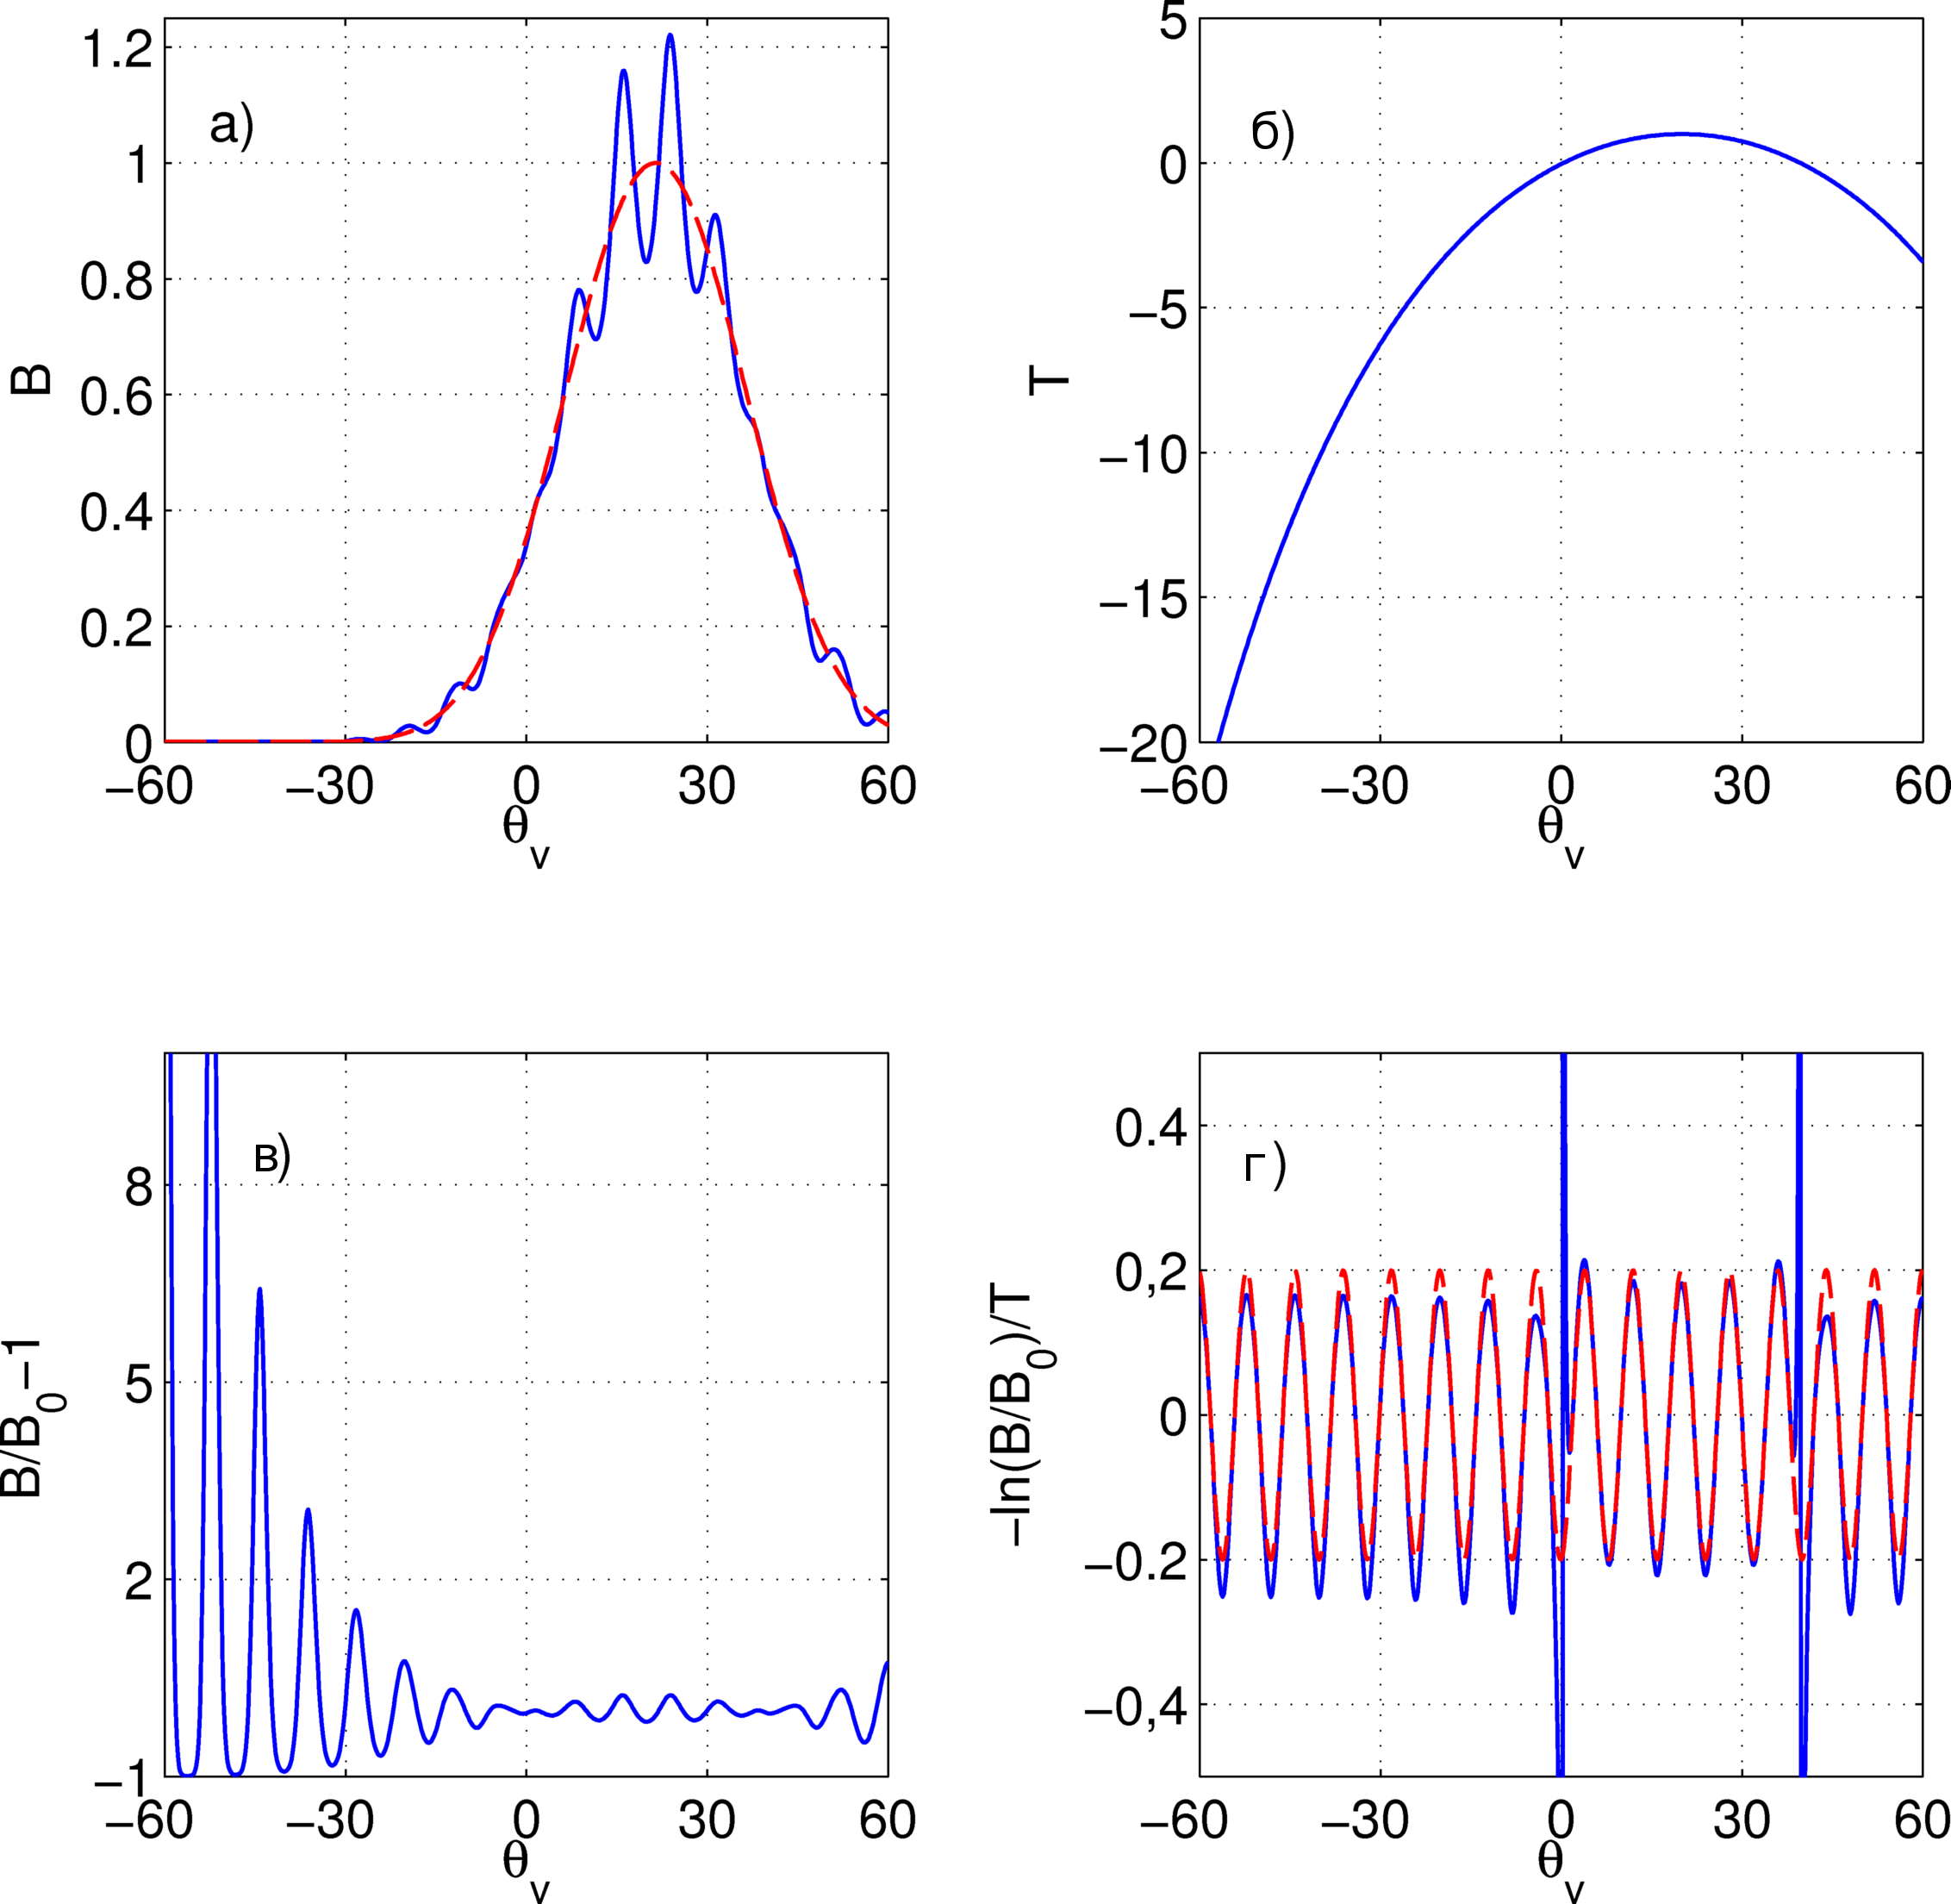
\includegraphics[width=\linewidth]{fig5}
    \floattitle{(a) Яркость солнечного блика (в относительных единицах) для спокойной $B_{0} $ (пунктирная линия) и возмущённой $B$ (сплошная линия) поверхности с СКН, заданным уравнением \eqref{eq:1.16}, в зависимости от угла наблюдения $\theta _{v} $ (в градусах); (б) передаточная функция \eqref{eq:1.15}; (в) относительные вариации яркости $(B-B_{0} )/B_{0} $; (г) сплошная линия -- вариации СКН, восстановленные по вариациям яркости, представленным на Рисунке~\ref{fig:5},~(в) с использованием передаточной функции $T$, показанной на Рисунке~\ref{fig:5},~(б), пунктирная линия -- исходные вариации СКН}
    \caption{Пример моделирования солнечного блика с передаточной функцией \eqref{eq:1.15}, для изотропной Гауссовой функции ПРВ}
    \label{fig:5}
\end{figure}



\newpage

\section{Применение метода к анализу данных MODIS и MERIS} \label{sec:1.4}



В данной работе основное внимание посвящено анализу спутниковых данных, получаемых с оптических сканеров MODIS (Moderate Resolution Imaging Spectroradiometer) и MERIS (MEdium Resolution Imaging Spectrometer), в том числе различиям и сходствам в подходах восстановления контрастов СКН по их изображениям. 

Сканеры MODIS установлены на двух спутниках Национального управления США по аэронавтике и исследованию космического пространства (NASA) Terra и Aqua. Сенсор MERIS, установленный на борту спутника Envisat, принадлежит Европейскому космическому агентству (ЕКА). Данные, получаемые с этих приборов, широко используются в научных исследованиях и различных практических приложениях. Эти данные общедоступны в сети интернет. Европейское космическое агентство (ЕКА) распространяет данные MERIS через ``роллинг'' архивы. Обычно файлы появляются на серверах уже через 3-- 6 часов после получения их спутником и удаляются через 10 дней (отсюда название ``роллинг'' архива). Данные MODIS доступны для скачивания с сайта \url{http://rapidfire.sci.gsfc.nasa.gov/}

Данные сканера MODIS представлены 36-ю каналами в видимом и инфракрасном (ИК) диапазонах, с пространственным разрешением 250м, 500м и 1км и точностью привязки, по меньшей мере, 50м \citep{Salomonson1989, Wolfe2002}. В свою очередь, данные прибора MERIS формируются 15-ю каналама с длинами волн от 390нм до 1040нм, с пространственным разрешением 300м и 1км, а точность привязки достигает 170м \citep{Goryl2004}.

Отличительной особенностью спутниковых изображений, полученных с приборов MODIS и MERIS в дневное время над водными бассейнами, являются серебристо-серые эллипсы отражённой солнечной радиации (солнечный блик), наблюдаемые при углах зеркального отражения около 30-- и градусов. Именно эти районы солнечного блика, где невозможны исследования оптических характеристик вод Океана (цвета Океана) \citep{Esaias1998}, могут быть использованы для исследования ``шероховатости поверхности Океана '' и проявления в ней различных океанических явлений. 

Напомним, что для исследования солнечного блика наиболее предпочтителен красный канал, поскольку свет в красном канале поглощается в ``тонком'' поверхностном слое Океана \citep{Jerlov1976}, и, таким образом, не так чувствителен к ``цвету'' водного столба, а также не чувствителен к поверхностной температуре.

Именно поэтому в работе используются данные уровня 1B, разрешением 250м первого (645нм) и второго (850нм) каналов для инструмента MODIS и данные восьмого (681нм) и тринадцатого (865нм) каналов MERIS высокого разрешения, сопровождаемые геолокационными данными и геометрией съемки.

MODIS является сканирующим спектрометром. Благодаря конструкции сканирующего зеркала, получаемые изображения представляют собой композицию полос 2330км длиной и около 10км шириной в надире. Каждая такая полоса формируется 40 детекторами с полем зрения вдоль и поперек траектории полета около 0.8${}^\circ$ и 110${}^\circ$, соответственно. Таким образом, каждая отдельная полоса содержит двумерное поле отраженной яркости. Внутри области солнечного блика эти особенности формирования изображений MODIS могут создавать ступенчатые изменения, -- эффект ``пилы'' (от англ. ``saw'' effect), отражённой от поверхности воды солнечной радиации при переходе от полосы к полосе (Рисунок~\ref{fig:6}). Поэтому в предлагаемом алгоритме исходное изображение MODIS в области солнечного блика делится на полосы и в дальнейшем двумерное поле яркости в каждой из полос обрабатывается отдельно.

MERIS -- спектрометр с постоянным сканированием. Он ведёт сканирование земной поверхности при помощи ПЗС матриц, обеспечивающих обзор поперёк траектории полета, а изображение вдоль полета формируется благодаря движению спутника. MERIS обладает широким углом обзора (68.5${}^\circ$) и шириной полосы 1150км в надире. Угол обзора в 68.5${}^\circ$ обеспечивается пятью одинаковыми оптическими камерами (Рисунок~\ref{fig:7}).

Угол обзора в направлении перпендикулярном направлению траектории полёта спутника у каждой из камер 14${}^\circ$. Угол обзора каждого пикселя составляет 0.019${}^\circ$. Благодаря широкому углу обзора всего инструмента 68.5${}^\circ$, пространственное разрешение поперёк движения спутника колеблется в пределах от 0.26~км в надире до 0.39~км по краям снимка. Разрешающая способность съёмки Земной поверхности вдоль движения спутника составляет 0.29~км.


\begin{figure}[H]
	\centering
	\begin{minipage}{.47\textwidth}
		\subcaptionbox{\label{fig:6a}}
	    {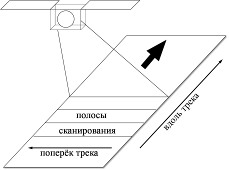
\includegraphics[width=1\linewidth]{fig6a}}
    \end{minipage}
    \hfill
    \begin{minipage}{.47\textwidth}
	    \subcaptionbox{\label{fig:6b}}
	    {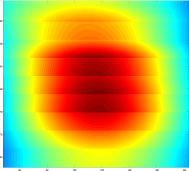
\includegraphics[width=1\linewidth]{fig6b}}
    \end{minipage}
    \\
    \floattitle{Хорошо видна ``полосообразная'' структура изображения в области солнечного блика с явно выраженными двумерными градиентами яркости вдоль и поперек траектории полета спутника}
    \caption{(а) Схематическая геометрия поля зрения прибора MODIS. (б) фрагмент изображения MODIS/Terra, 24 мая 2010г., 16ч. 45мин., район разлива нефтепродуктов в результате взрыва нефтяной платформы ``Deepwater Horizon'' в Мексиканском заливе}
    \label{fig:6}

	\centering
	\begin{minipage}{.47\textwidth}
	    \subcaptionbox{\label{fig:7a}}
		{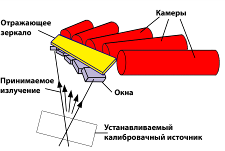
\includegraphics[width=1\linewidth]{fig7a}}
	\end{minipage}
	\hfill
	\begin{minipage}{.47\textwidth}
	    \subcaptionbox{\label{fig:7b}}
		{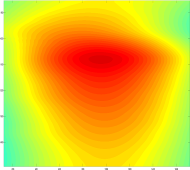
\includegraphics[width=1\linewidth]{fig7b}}
	\end{minipage}
	\\
    \floattitle{В отличие от изображения MODIS на Рисунке~\ref{fig:6},~(б), в данном случае поле яркости в солнечном блике не имеет полос сканирования
}
    \caption{(а) Схематическое устройство прибора MERIS/Envisat (б) фрагмент изображения MERIS, 24 мая 2010г., 16ч. 17мин., в Мексиканском заливе}
    \label{fig:7}
\end{figure}



\newpage

\section{Программа восстановления СКН по полям яркости}

Ниже приводится пошаговая процедура чтения, обработки и восстановления СКН на примере спутниковых снимков MODIS и MERIS района течения Гольфстрим у берегов Флориды.



\subsection{Среда и языки программирования}

Все разработанные алгоритмы, процедуры загрузки, чтения и обработки спутниковой и другой вспомогательной информации, описанные в диссертации, реализованы на языках программирования Matlab (\url{http://www.mathworks.com/products/matlab/}) и, частично, Python (\url{http://www.python.org/}). На программу, реализующую предложенный алгоритм, получен патент \citep{mag2011}: ``GLAMOROS: Оценка контрастов поверхностных проявлений океанических явлений по изображениям солнечного блика''.

MATLAB (сокращение от англ. ``Matrix Laboratory'', в русском языке произносится как Матл\'{а}б) -- пакет прикладных программ для решения задач технических вычислений и одноимённый язык программирования, используемый в этом пакете.

Python (англ. Python -- питон, произносится па\'{й}тон; в русском языке распространено название пит\'{о}н) -- высокоуровневый язык программирования общего назначения, ориентированный на повышение производительности разработчика и читаемости кода.



\subsection{Данные MODIS и MERIS, используемые в примере}

Для демонстрации возможностей разработанного алгоритма применим его к изображениям района течения Гольфстрим. Течение Гольфстрим достаточно хорошо изучено и характеризуется разнообразием проявляемой на спутниковых изображениях мезомасштабной динамики (вихри, грибовидные структуры, температурные фронты, внутренние волны, зыбь и многие другие явления проявления океанической динамики).

Данные MERIS, а также MODIS/Terra и MODIS/Aqua в районе исследования были получены 01~Апреля 2010~г. в 15 ч.~42 мин., 16 ч.~30 мин. и 18 ч.~05 мин., соответственно.

RGB композитные изображения MODIS/Terra, MERIS и MODIS/Aqua района исследования приведены на Рисунке~\ref{fig:8},. Отчётливо видно, что солнечный блик на псевдо-цветных оптических изображениях проявляется в виде серебристых эллипсов.



\begin{figure}[!thb]
    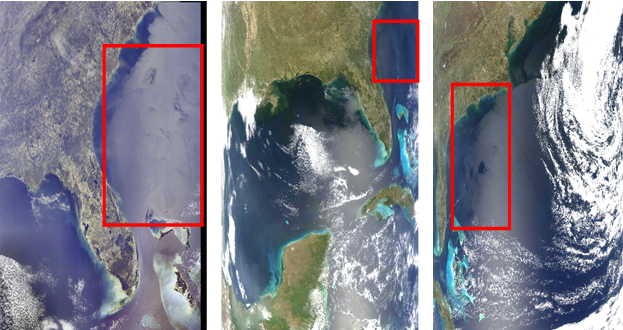
\includegraphics[width=\linewidth]{fig8}
    \floattitle{Слева направо: MERIS, MODIS/Terra и MODIS/Aqua в районе исследования были получены 01 Апреля 2010 г. в 15 ч. 42 мин., 16 ч. 30 мин. и 18 ч. 05 мин., соответственно. Красным контуром отмечены области, по которым будет приведён пример работы разработанного подхода, алгоритмов и соответствующего программного обеспечения}
    \caption{Псевдо-цветные RGB изображения района течения Гольфстрим у берегов Флориды}
    \label{fig:8}
\end{figure}




\subsection{Процедура восстановления СКН по спутниковым оптическим изображениям}

Обобщение этапов процедуры восстановления СКН по спутниковым оптическим изображениям MODIS и MERIS представлено в виде линейной алгоритмической структуры на Рисунке~\ref{fig:9}. Эта процедура состоит из следующих этапов:



\begin{enumerate}
\item Вспомогательные данные
	\begin{enumerate}
		\item Загрузка и чтение данных, включая данные геолокации и геометрии наблюдений
		\item Cоздание масок земли и облаков
		\item Построение полей ветра
	\end{enumerate}
\item Выбор района исследования на изображении (в красном канале)
\item Построение контрастов яркости
	\begin{enumerate}
		\item Определение среднего поля яркости
		\item Построение поля флуктуаций яркости
		\item Устранение эффекта ``пилы'' для MODIS
	\end{enumerate}
\item Нахождение передаточной функции связи контрастов яркости и контрастов СКН
\item Восстановление СКН
\item Построение карт зон инверсии контрастов
\item Расчёт карт локальных наклонов морской поверхности
\end{enumerate}



\begin{figure}[H]
    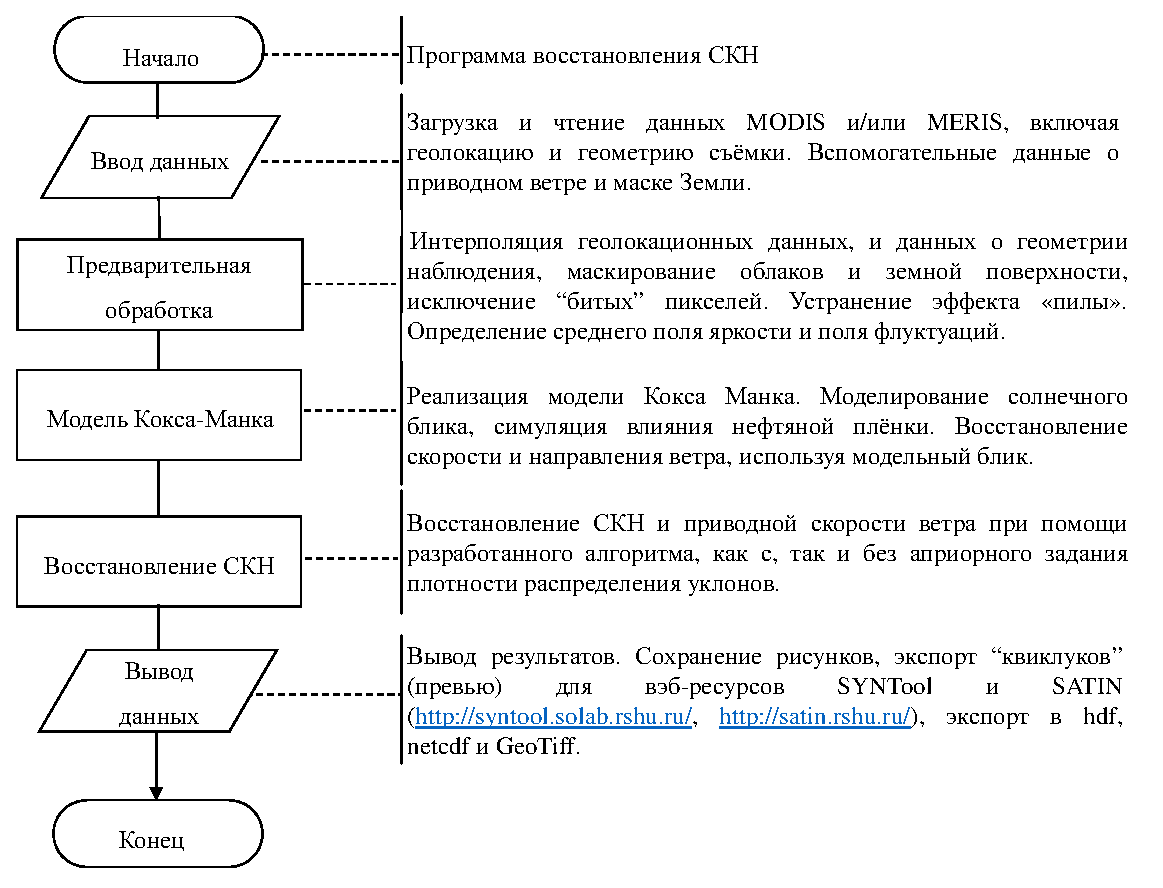
\includegraphics[width=\linewidth]{fig9.eps}
    \floattitle{Линейная алгоритмическая структура, отражающая основные аспекты процедуры восстановления СКН по спутниковым оптическим изображениям MODIS и MERIS}
    \caption{Блок-схема алгоритма восстановления СКН}
    \label{fig:9}
\end{figure}



\subsubsection{Вспомогательные данные}

Прежде чем приступать непосредственно к обработке данных, были написаны скрипты для загрузки и чтения данных MODIS и MERIS, включая файлы с геолокацией и геометрией съёмки, а также вспомогательные данные о приводном ветре и маске Земли.

В качестве маски земли использовались данные GTOPO30 \citep{USGS1996gtopo30}. GTOPO30 - цифровая модель рельефа (англ. Global 30 Arc-Second Elevation Data Set), разработанная в геологической службе США (англ. USGS - United States Geological Survey).

В качестве источника данных о скорости и направлении приводного ветра использовались модельный ветер NCEP GFS \citep{ncep} и ветер, интерполированный с различных скаттерометров, Blended Sea Winds \citep{Zhang2006}.

Функционирование глобальной системы прогнозирования GFS (англ. Global Forecast System), осуществляется NCEP (англ. National Centers for Environmental Prediction, Национальные центры для предсказания окружающей среды), которые являются подразделением NOAA (англ. National Oceanic and Atmospheric Administration, Национальное управление океанических и атмосферных исследований), NWS (National Weather Service, Национальная служба погоды), США. GFS модель обновляется четыре раза в день (00:00, 06:00, 12:00 и 18:00 UTC) на 384 часа. Начиная с июля 2010 года модель обновляется с разрешением в 27км (ранее 35км) на 192 часа и затем с меньшим разрешением до 384 часов. Файлы с данными GFS, которые на данный момент предоставляются NOAA, имеют разрешение в 0.5 градуса (примерно 50км) что является действительным разрешением прогнозов обозримых на этом или других сайтах использующих тот же источник.

Альтернативным продуктом с полями скорости ветра является Blended Sea Winds -- продукт NOAA, содержащий как скорость и направление ветра и ветровые напряжения, с пространственным разрешением 0.25${}^\circ$. Описание и данные доступны в статье \citep{Zhang2006} и соответствующих ссылках.

Карты полей ветра в районе исследования приведены на Рисункe~\ref{fig:wind}.



\begin{figure}[H]
   	\centering
	\begin{minipage}{.47\textwidth}
	    \subcaptionbox{\label{fig:windA}}
		{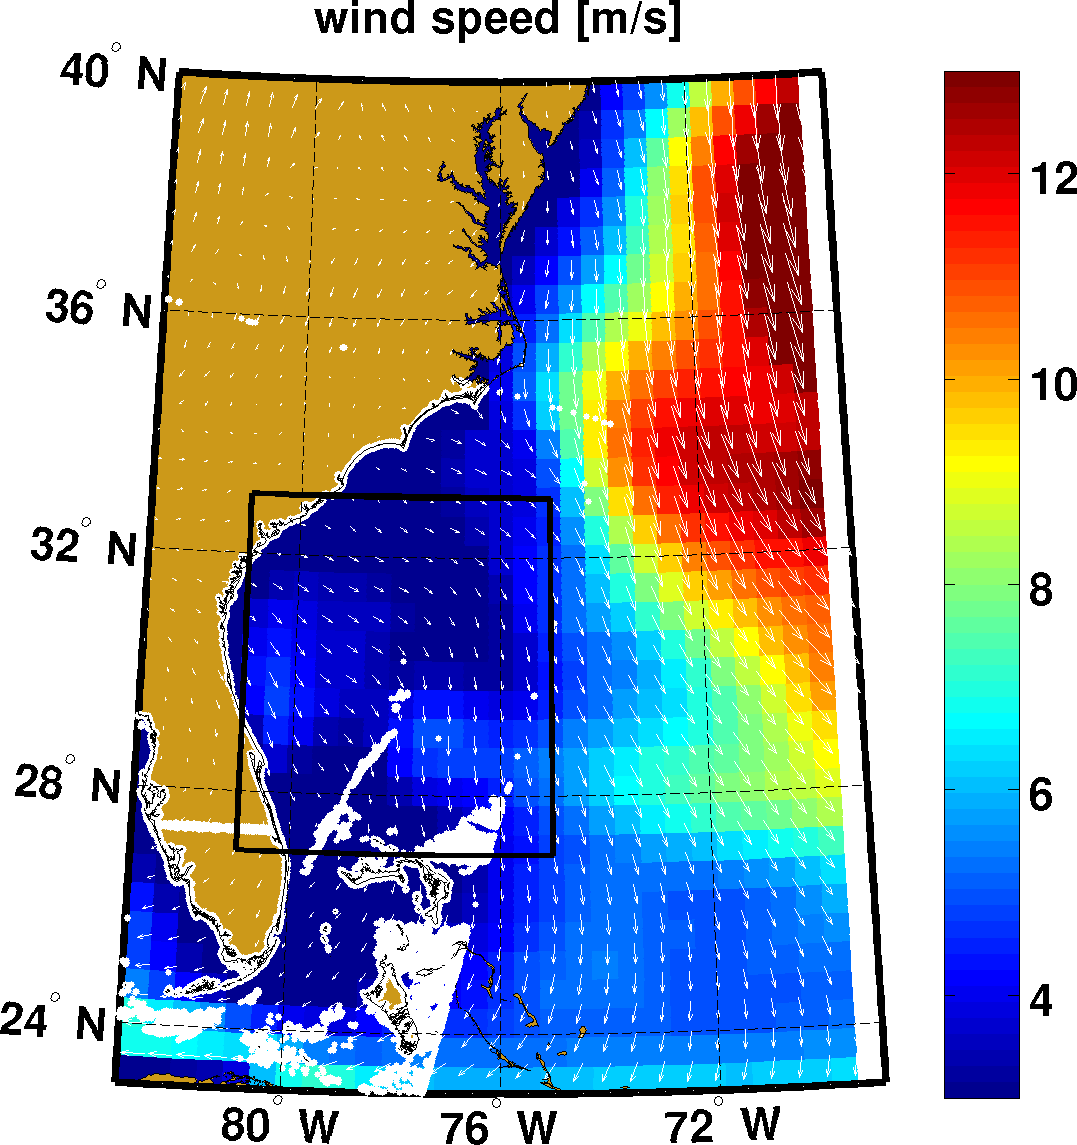
\includegraphics[width=1\linewidth]{windA}}
	\end{minipage}
	\hfill
	\begin{minipage}{.47\textwidth}
	    \subcaptionbox{\label{fig:windB}}
		{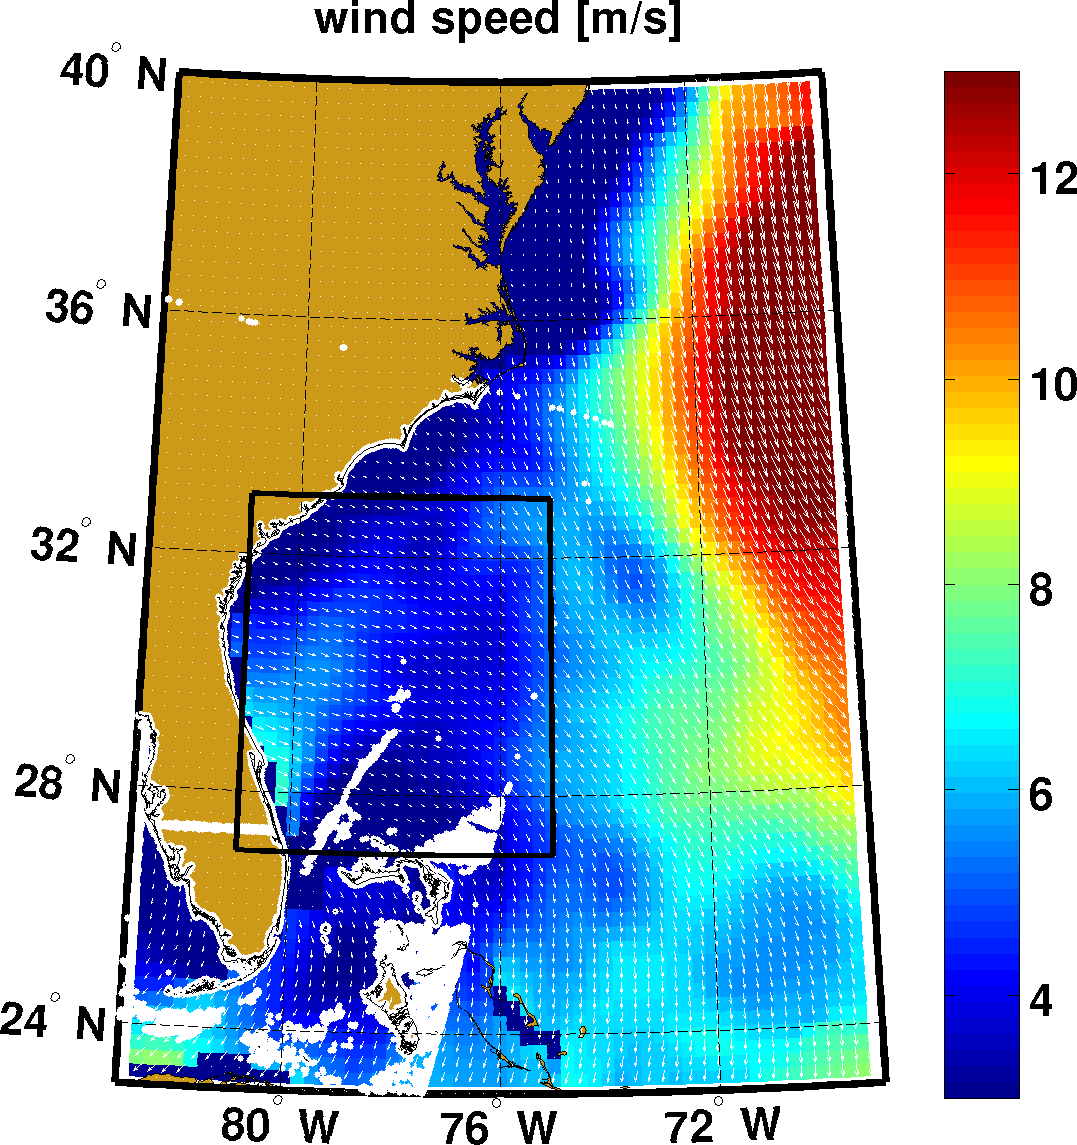
\includegraphics[width=1\linewidth]{windB}}
	\end{minipage}
	\\
	\begin{minipage}{.47\textwidth}
	    \subcaptionbox{\label{fig:windC}}
		{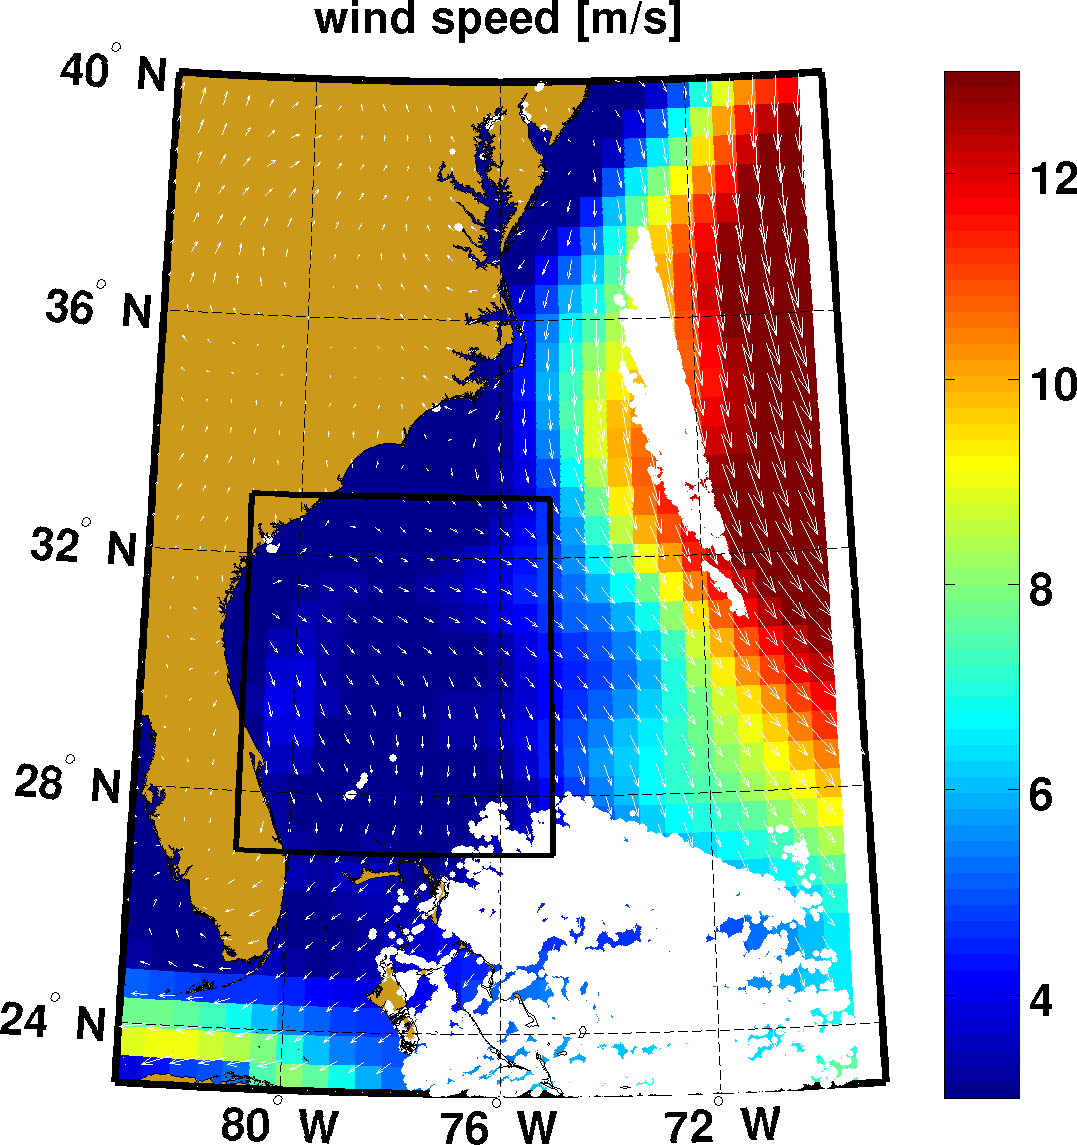
\includegraphics[width=1\linewidth]{windC}}
	\end{minipage}
	\hfill
	\begin{minipage}{.47\textwidth}
	    \subcaptionbox{\label{fig:windD}}
		{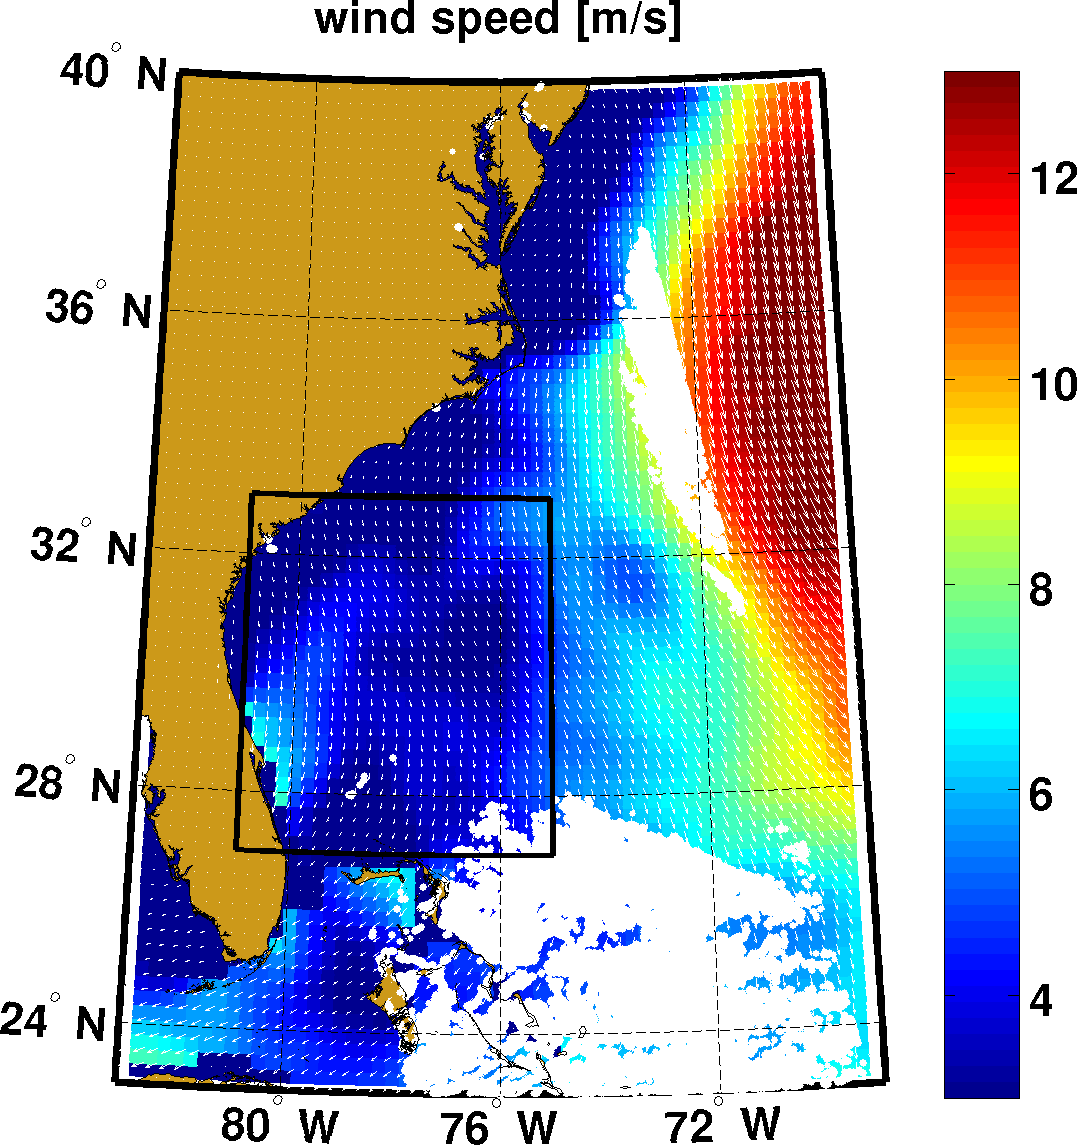
\includegraphics[width=1\linewidth]{windD}}
	\end{minipage}
    \\
    \floattitle{(а) и (в) -- скорость и направление ветра в 15 и 18 часов 01 Апреля 2010г., соответственно, взятые из модели NCEP GFS.
    (б) и (г) -- скорость и направление ветра в 15 и 18 часов 01 Апреля 2010г., соответственно, построенные по данным Blended Sea Winds.
    Здесь и далее, чёрным контуром выделен район выбранный для дальнейшего исследования, коричневым цветом нанесена маска Земли, а белым -- облаков.}
    \caption{Карты полей ветра в районе исследования, построенные по данным NCEP GFS и Blended Sea Winds}
    \label{fig:wind}
\end{figure}

На представленных картах полей ветра, отчётливо видно что разрешающая способность данных NCEP GFS (0.5${}^\circ$) ниже Blended Sea Winds (0.25${}^\circ$). Также стоит отметить, что скорость и направление ветра существенно не изменились за три часа, и, соответственно, за время наблюдения этого района приборами MERIS и MODIS спутников Envisat и Aqua/Terra. Средняя скорость в районе исследования составляла около 3-5м/c. Эти значения помогут нам в дальнейшем анализировать обработанные изображения.

На Рисунке~\ref{fig:11} приводится область исследования, ``вырезанная'' из исходных изображений MERIS, MODIS/Terra и MODIS/Aqua, в красных (865нм для MERIS и 850нм для MODIS) каналах, соответственно. Для примера взяты достаточно большие фрагменты трёх изображений, чтобы показать общий вид района. Далее из этих фрагментов будет выбрана лишь небольшая область у Восточного побережья США, отмеченная красным контуром на Рисунке~\ref{fig:8}, чтобы проиллюстрировать многообразие явлений на поверхности Океана и показать, как работает предложенный алгоритм и программы обработки в разных ситуациях. Геометрия наблюдений отличается на всех трёх примерах. Мы чётко видим блик на изображениях MERIS и MODIS/Aqua, а на фрагменте MODIS/Terra блик находится вне области исследования, а если быть точнее, в Мексиканском заливе, со стороны западного побережья Флориды, как видно из Рисунка~\ref{fig:7},. Для случая с MODIS/Terra, несмотря на то, что мы находимся на периферии блика, всё равно наблюдаем градиенты яркости, которые достаточны, чтобы проводить обработку изображения с применением предложенного подхода.



\begin{figure}[H]
    	\centering
	\begin{minipage}{.31\textwidth}
	    \subcaptionbox{\label{fig:11a}}
		{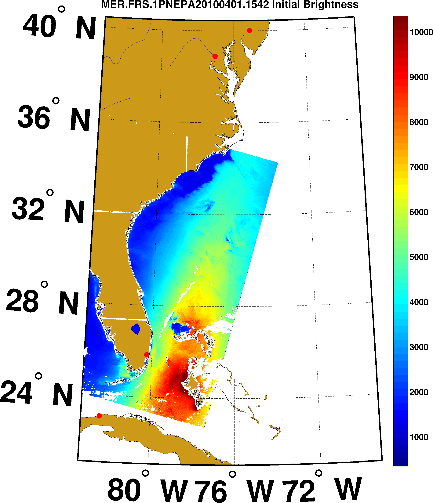
\includegraphics[width=1\linewidth]{fig11a}}
	\end{minipage}
	\hfill
	\begin{minipage}{.31\textwidth}
	    \subcaptionbox{\label{fig:11b}}
		{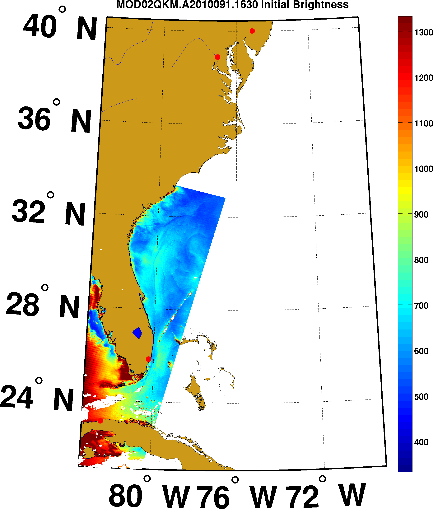
\includegraphics[width=1\linewidth]{fig11b}}
	\end{minipage}
	\hfill
	\begin{minipage}{.31\textwidth}
	    \subcaptionbox{\label{fig:11c}}
		{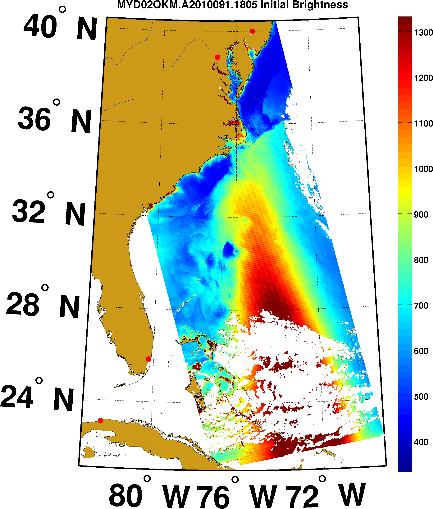
\includegraphics[width=1\linewidth]{fig11c}}
	\end{minipage}
	\\
    \floattitle{(а) MERIS, (б) MODIS/Terra, (в) MODIS/Aqua. Изображения получены 01 Апреля 2010 г. в 15 ч. 42 мин., 16 ч. 30 мин. и 18 ч. 05 мин., соответственно}
    \caption{Фрагменты изображений MERIS, MODIS/Terra и MODIS/Aqua в красных (865нм для MERIS и 850нм для MODIS) каналах}
    \label{fig:11}
\end{figure}

Таким образом, дальнейшая обработка изображений будет проведена по району, выделенному красным контуром на Рисунке~\ref{fig:8}. Выбранная область исследования, между 27${}^\circ$ и 33${}^\circ$~С.Ш. и 69${}^\circ$ и 83${}^\circ$~З.Д., приведена на Рисунке~\ref{fig:11}.

Прежде чем применить алгоритм к изображениям, производится интерполяция геолокационных данных и данных о геометрии наблюдения, маскирование облаков и земной поверхности, исключение ``битых'' пикселей. Далее, для восстановления СКН с помощью разработанного алгоритма без априорного задания плотности распределения уклонов, следуя выражениям \eqref{eq:1.6} и \eqref{eq:1.7}, необходимо исходные яркости изображения в красном канале представить в виде суммы среднего значения $\overline{B}$ (см. Рисунок~\ref{fig:14}) и вариаций $\widetilde{B}$ (см. Рисунок~\ref{fig:15}).



\begin{figure}[H]
    	\centering
	\begin{minipage}{.31\textwidth}
	    \subcaptionbox{\label{fig:12a}}
		{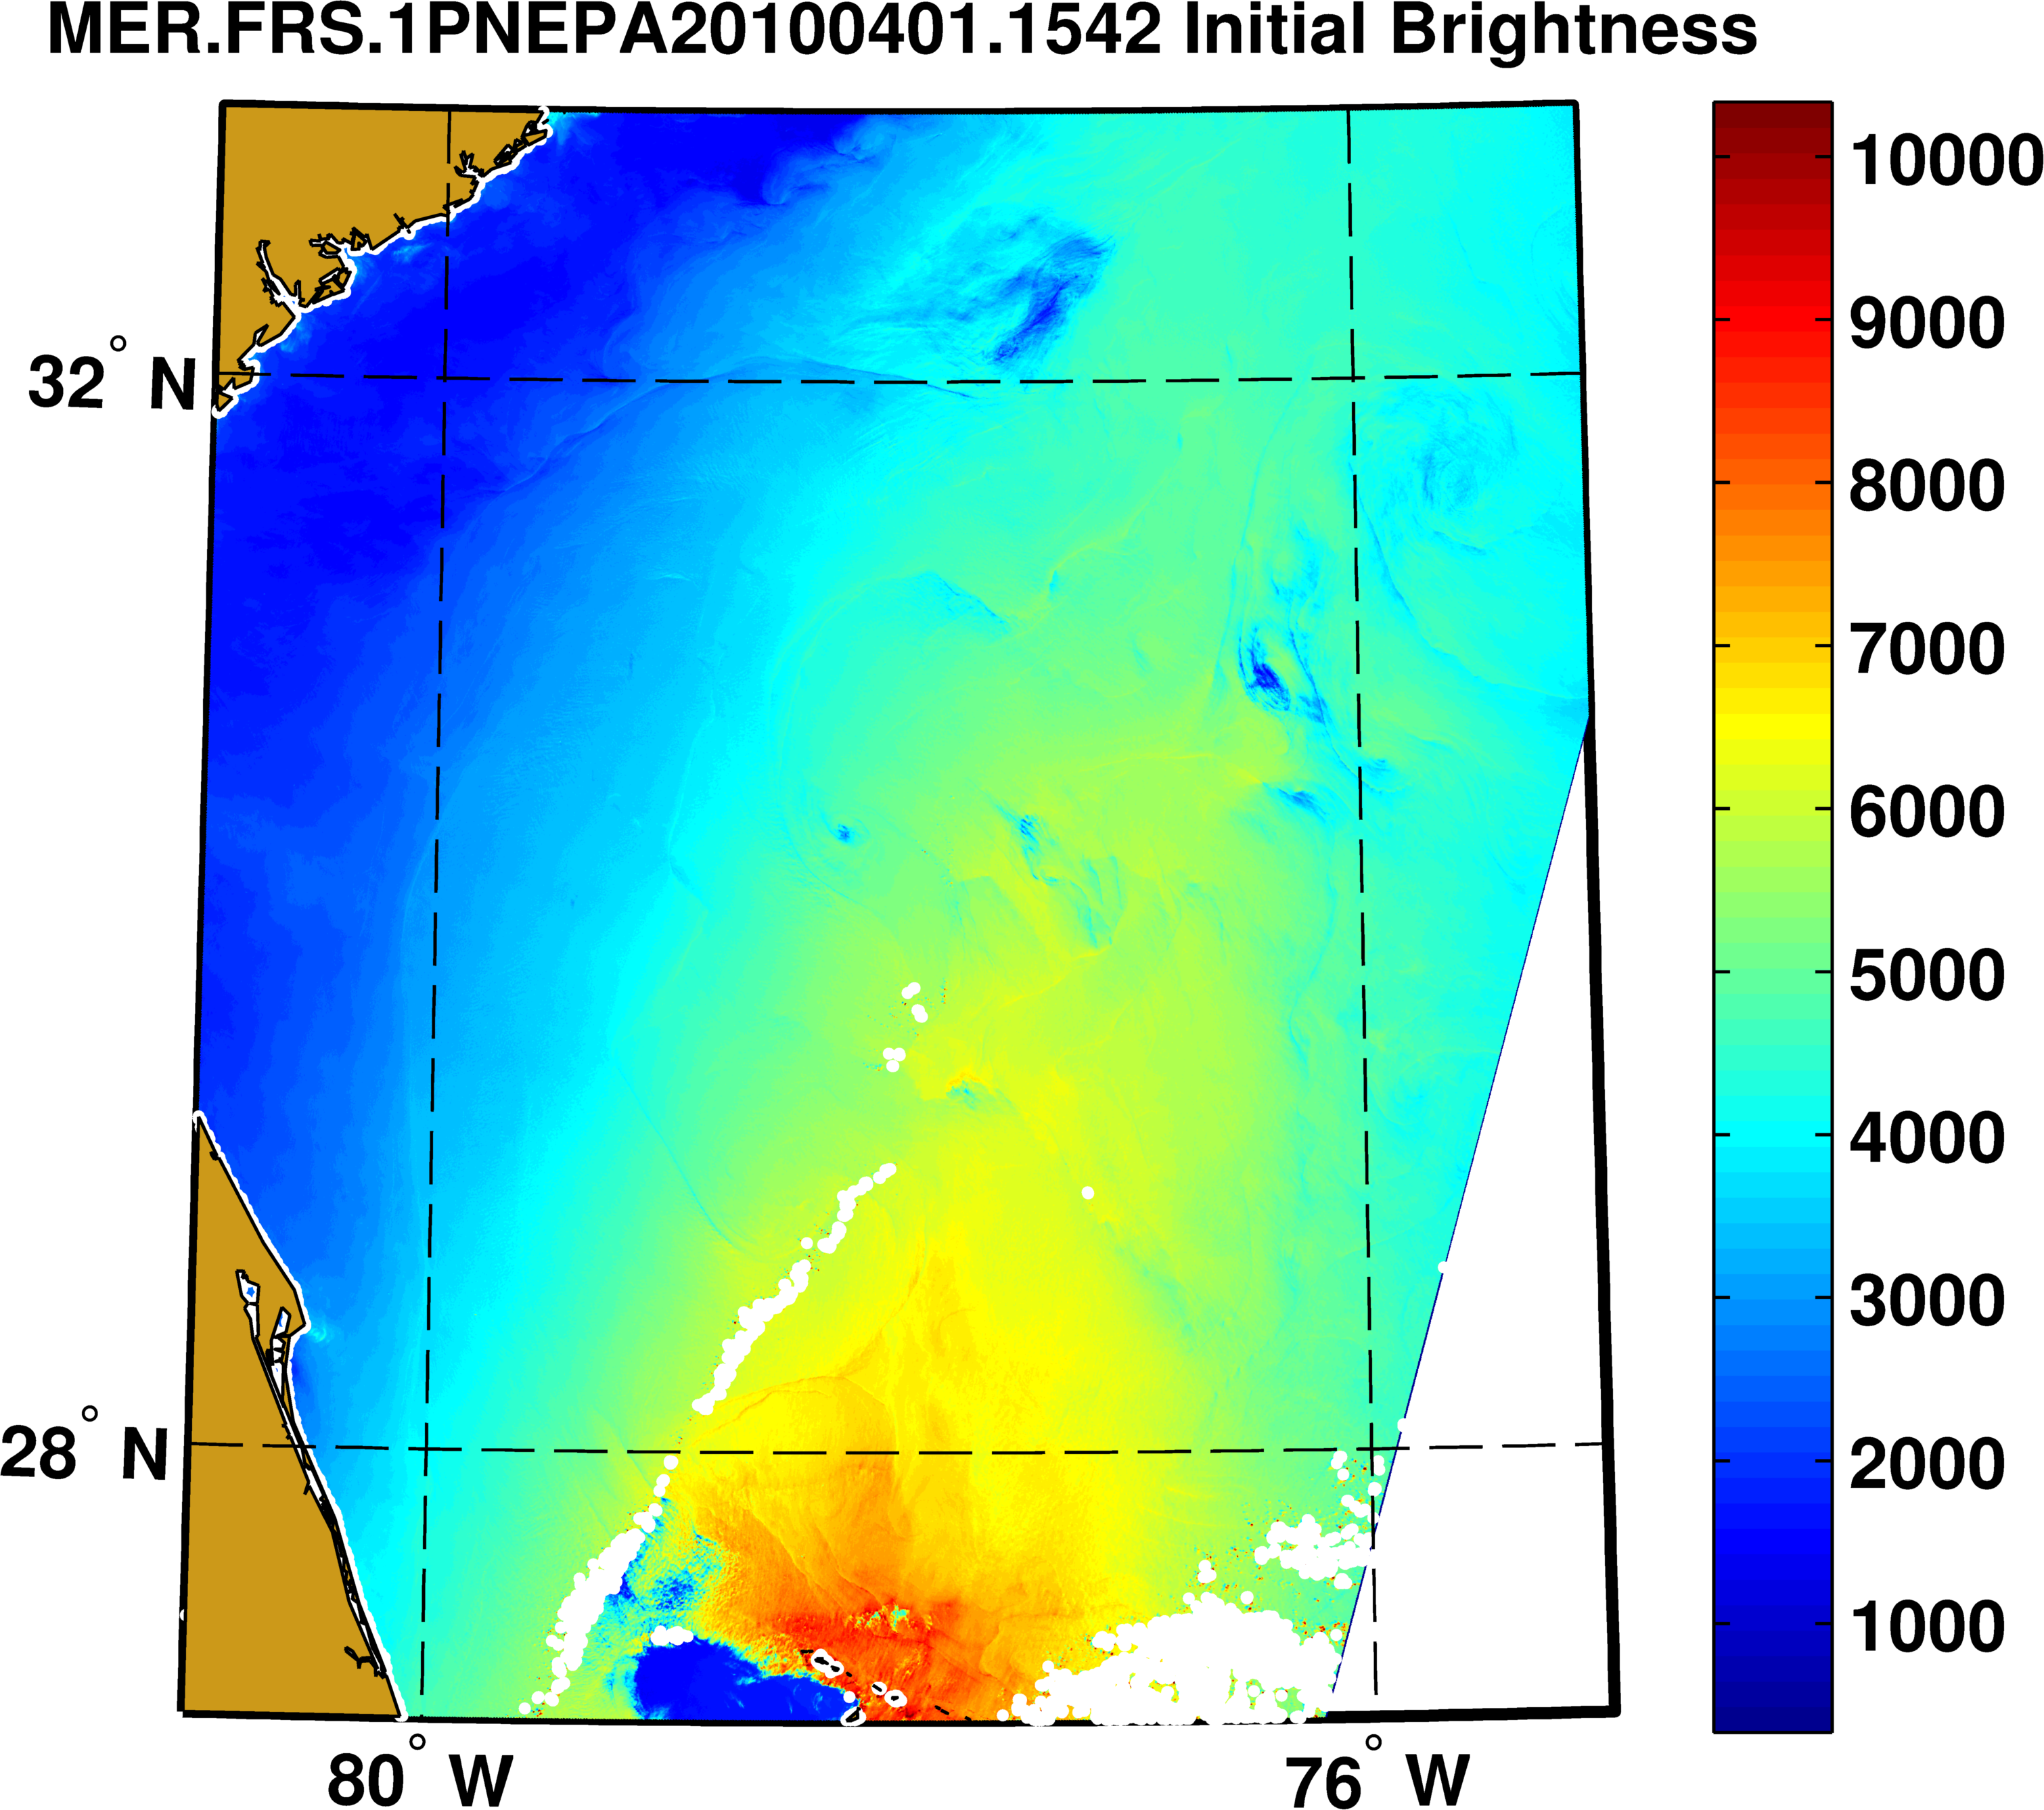
\includegraphics[width=1\linewidth]{fig12a}}
	\end{minipage}
	\hfill
	\begin{minipage}{.31\textwidth}
	    \subcaptionbox{\label{fig:12b}}
		{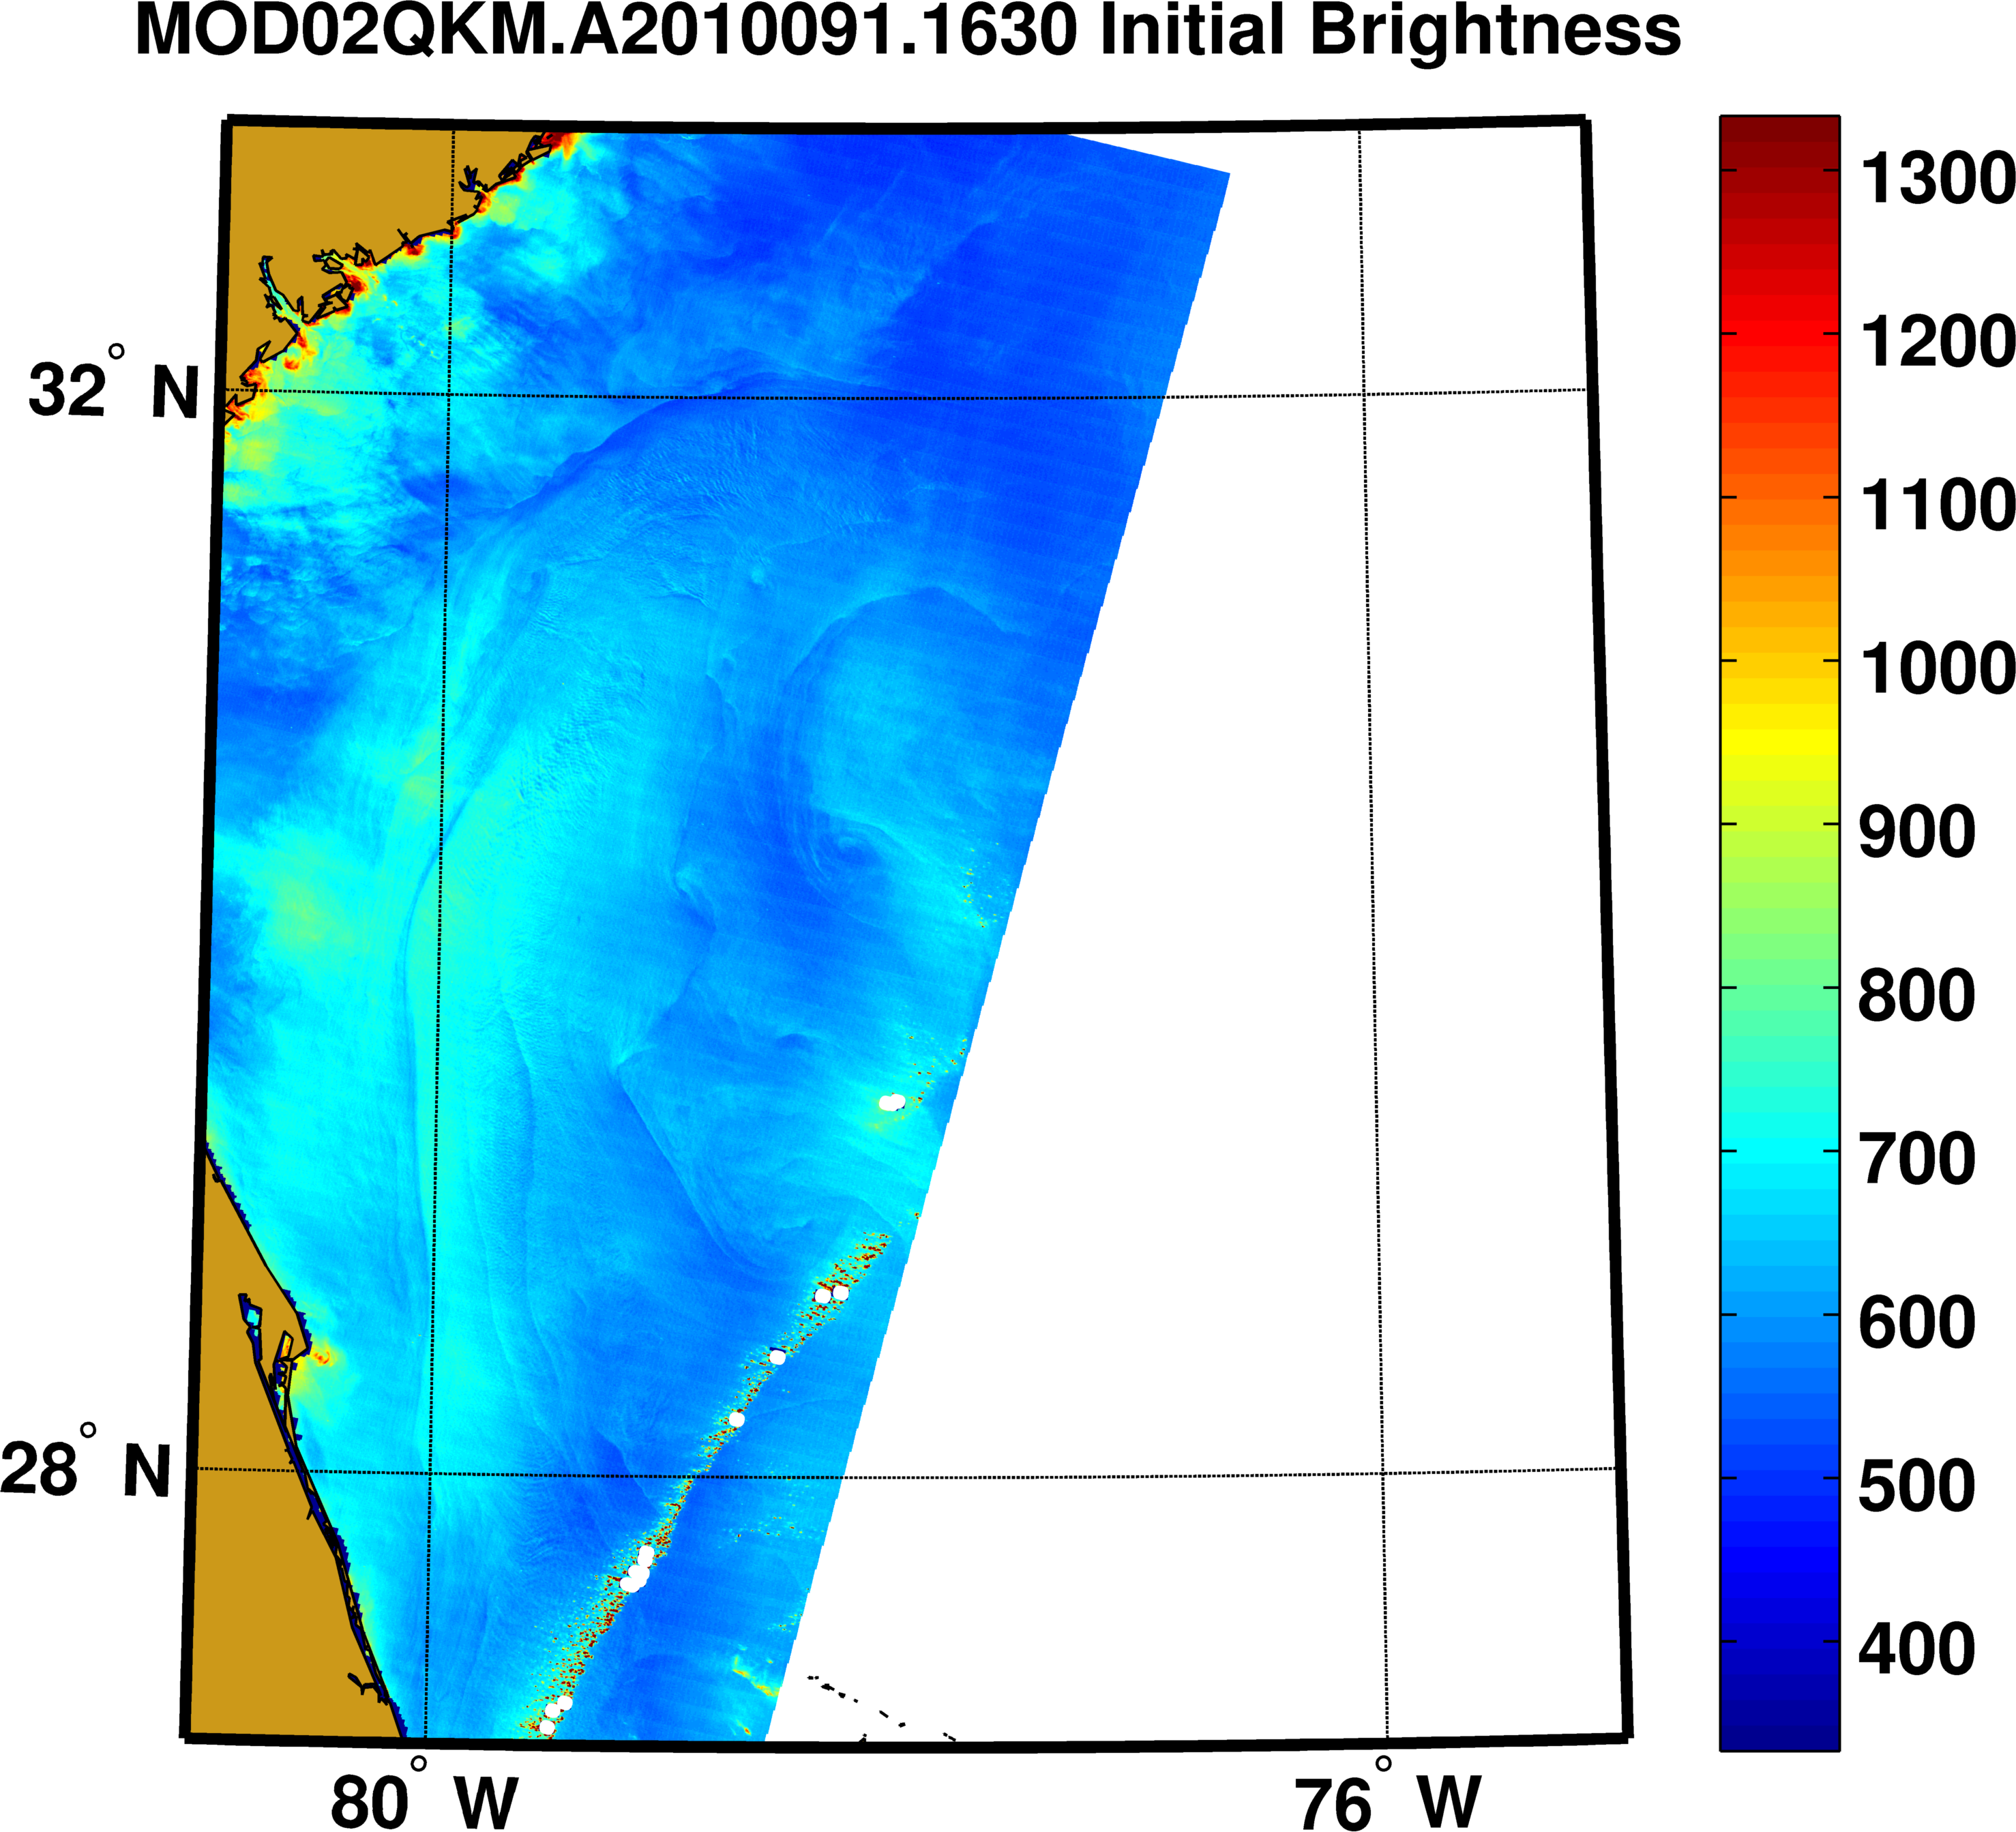
\includegraphics[width=1\linewidth]{fig12b}}
	\end{minipage}
	\hfill
	\begin{minipage}{.31\textwidth}
	    \subcaptionbox{\label{fig:12c}}
		{\includegraphics[width=1\linewidth]{fig12c}}
	\end{minipage}
	\\
	\floattitle{MERIS (а), MODIS/Terra (б) и MODIS/Aqua (в)}
    \caption{Область исследования на изображениях MERIS (а), MODIS/Terra (б) и MODIS/Aqua (в) в красных каналах}
    \label{fig:12}
\end{figure}

На Рисунке~\ref{fig:13} представлен пример сечения вдоль (б) и поперёк (а) блика, взятого для изображения MODIS/Aqua, на Рисунке~\ref{fig:11},~(а). На сечении, взятом вдоль блика (б) отчётливо видна ``пилообразная'' структура, описанная в разделе 1.3. Также из рисунка видно наличие 2D поля яркости солнечного блика, благодаря чему передаточная функция в \eqref{eq:1.7} может быть определена по усредненным градиентам яркости, которые берутся непосредственно из изображения солнечного блика, путём осреднения скользящим средним, с задаваемым окном.



\begin{figure}[H]
    	\centering
	\begin{minipage}{.47\textwidth}
	    \subcaptionbox{\label{fig:13a}}
		{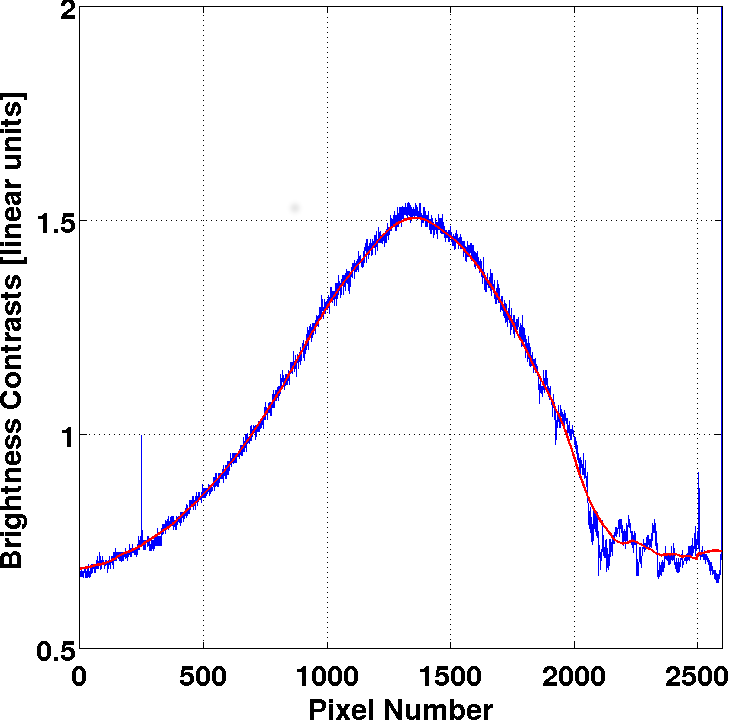
\includegraphics[width=1\linewidth]{fig13a}}
	\end{minipage}
	\hfill
	\begin{minipage}{.47\textwidth}
	    \subcaptionbox{\label{fig:13b}}
		{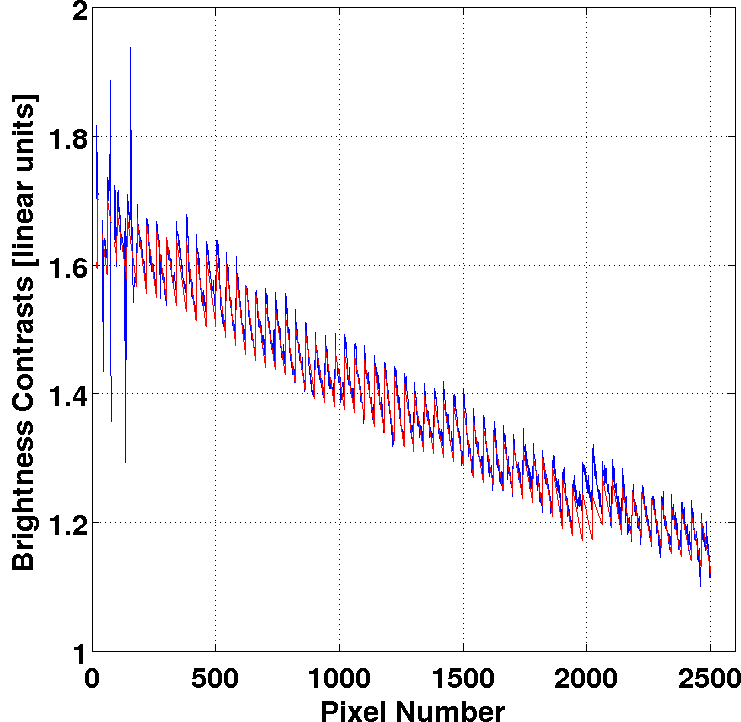
\includegraphics[width=1\linewidth]{fig13b}}
	\end{minipage}
	\\
    \floattitle{Пример сечения вдоль (б) и поперёк (а) блика, взятое для контрастов яркости изображения MODIS/Aqua вдоль одной из строк и столбца исходной матрицы изображения. Исходное изображение в красном канале представлено на Рисунке~\ref{fig:11},~(а). Синим цветом изображены исходные яркости в красном канале, а красным -- усреднённые. На сечении, взятом вдоль блика (б), отчётливо видна ``пилообразная'' структура (см. раздел 1.3), которая устраняется в результате обработки}
    \caption{Сечения контрастов яркости вдоль (б) и поперёк (а) блика}
    \label{fig:13}
\end{figure}




Вместе с определением среднего поля яркости и поля флуктуаций, разработанный способ разделения исходных яркостей также позволил добиться устранения эффекта ``пилы''.

Поля средней яркости солнечного блика (масштаб осреднения 30x30~км${}^2$) для данных MERIS и MODIS представлены на Рисунке~\ref{fig:14}.

\begin{figure}[H]
    	\centering
	\begin{minipage}{.31\textwidth}
	    \subcaptionbox{\label{fig:14a}}
		{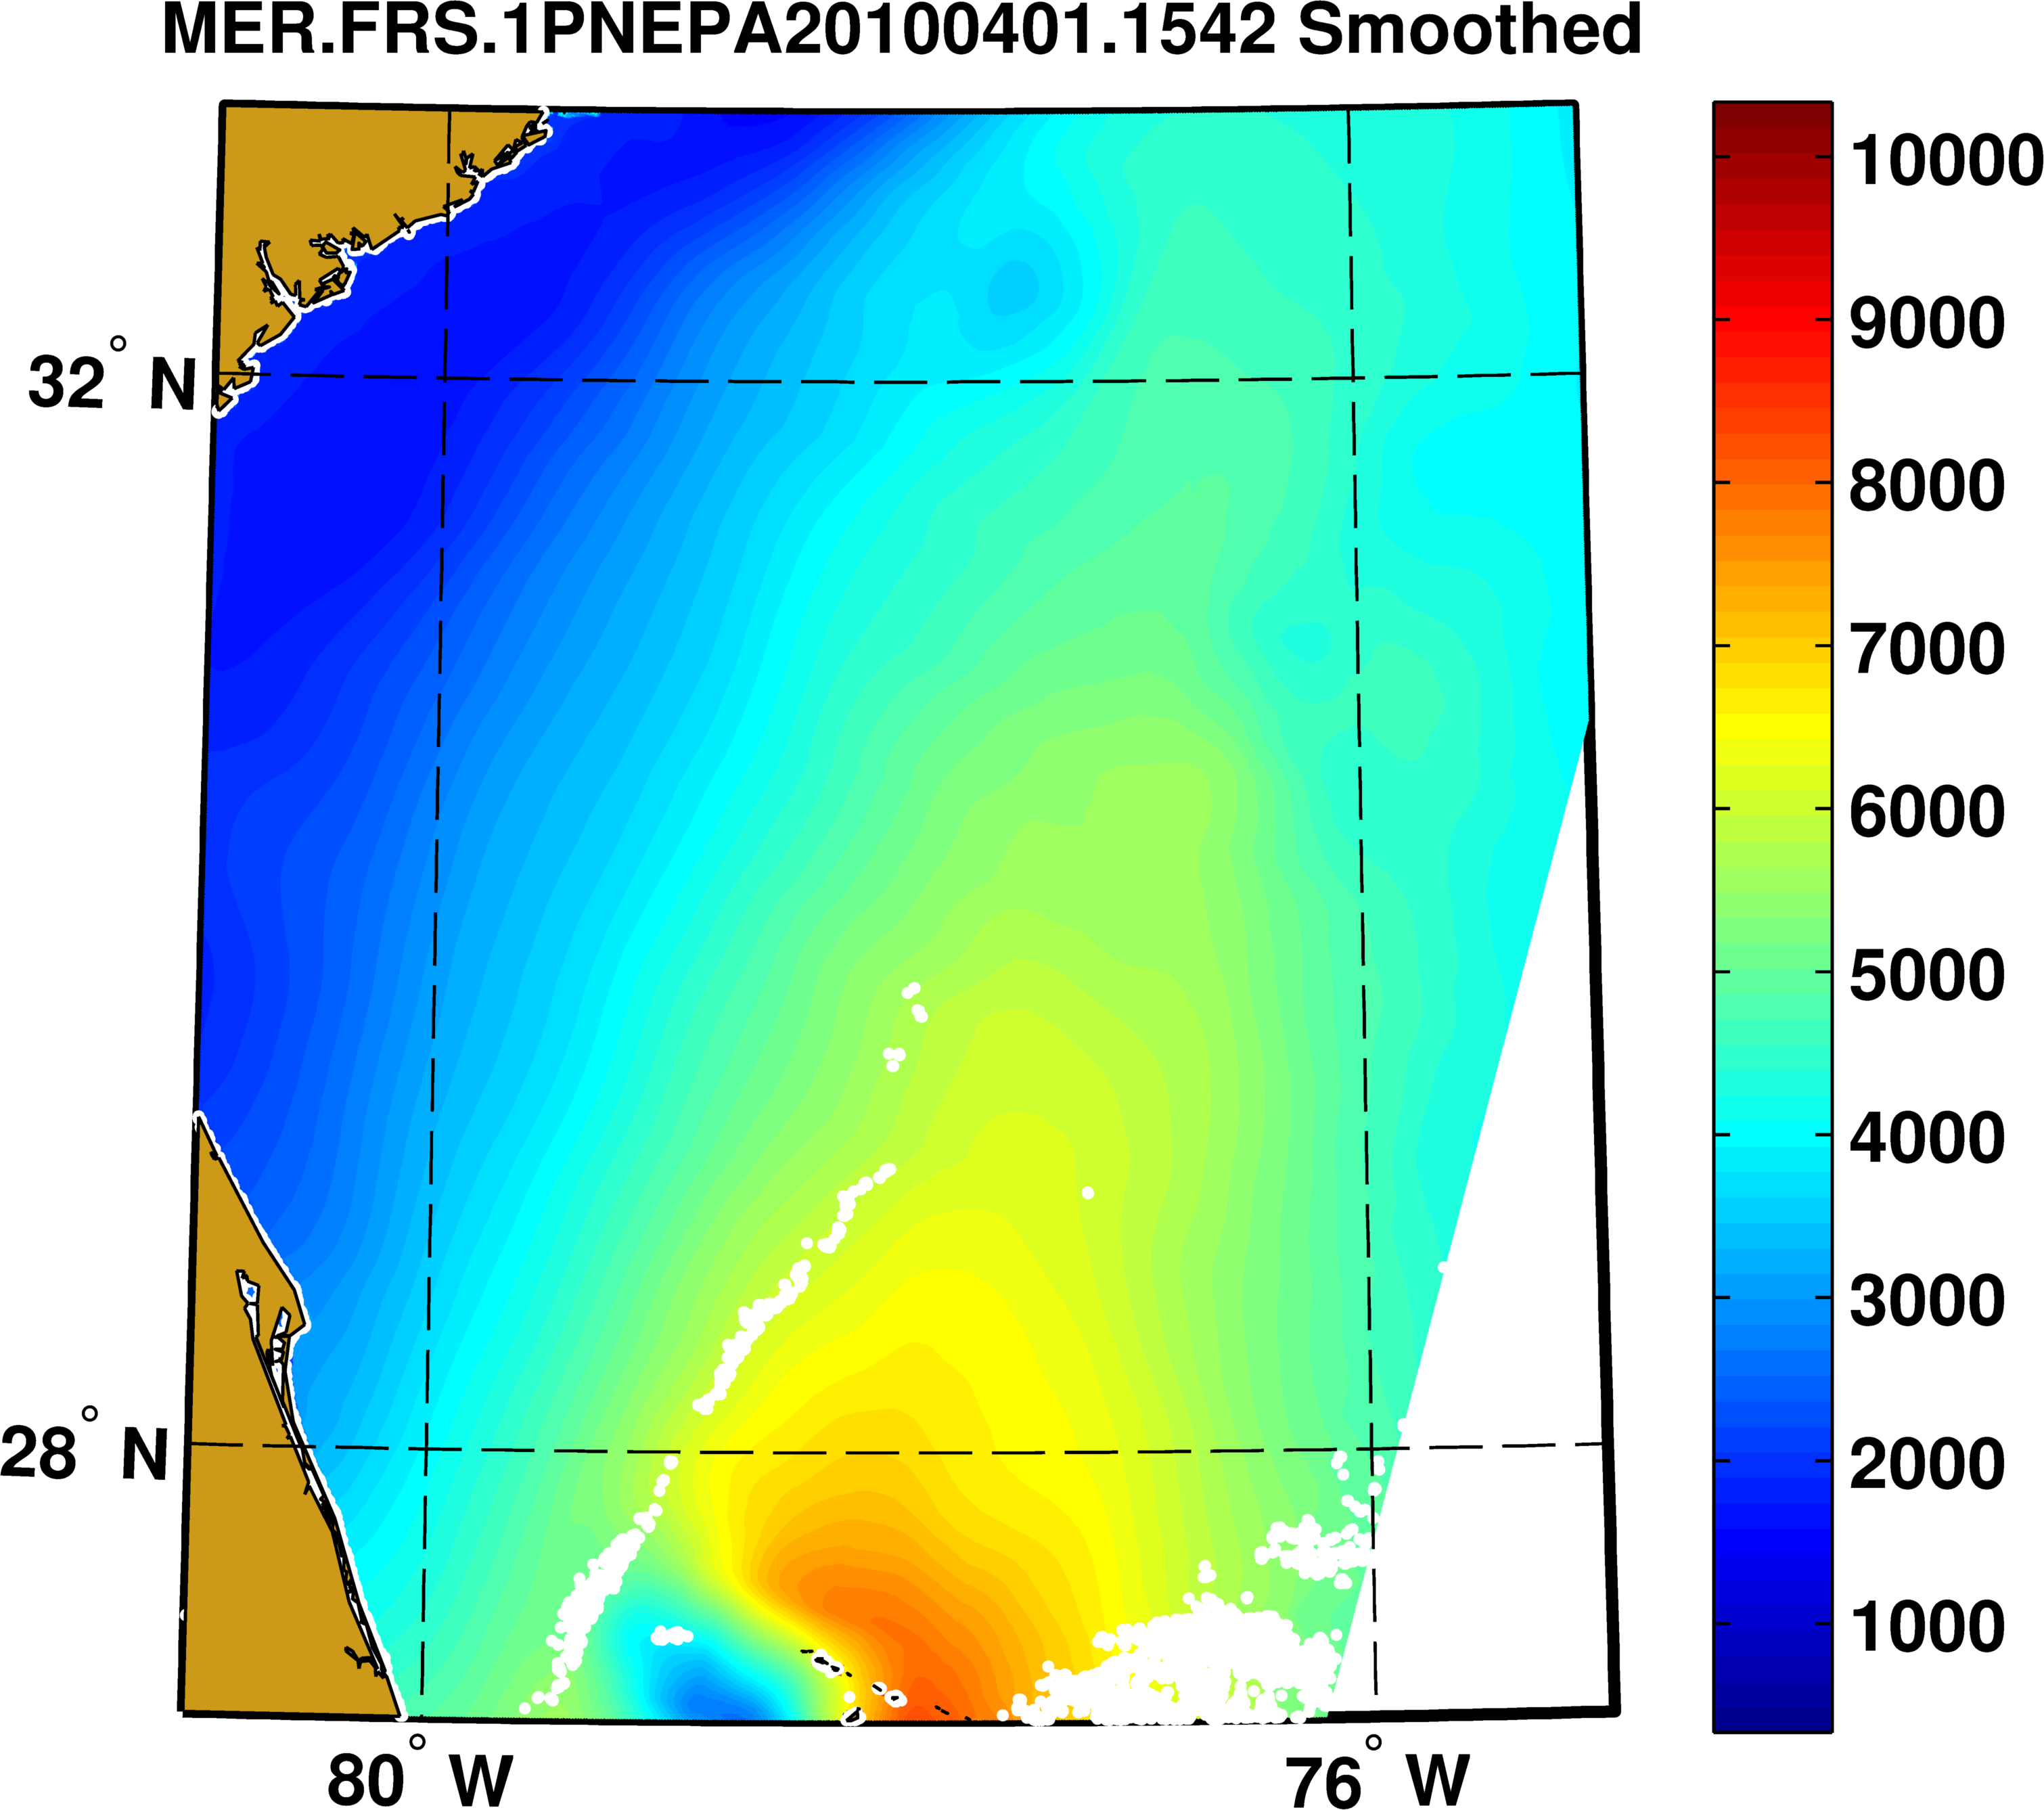
\includegraphics[width=1\linewidth]{fig14a}}
	\end{minipage}
	\hfill
	\begin{minipage}{.31\textwidth}
	    \subcaptionbox{\label{fig:14b}}
		{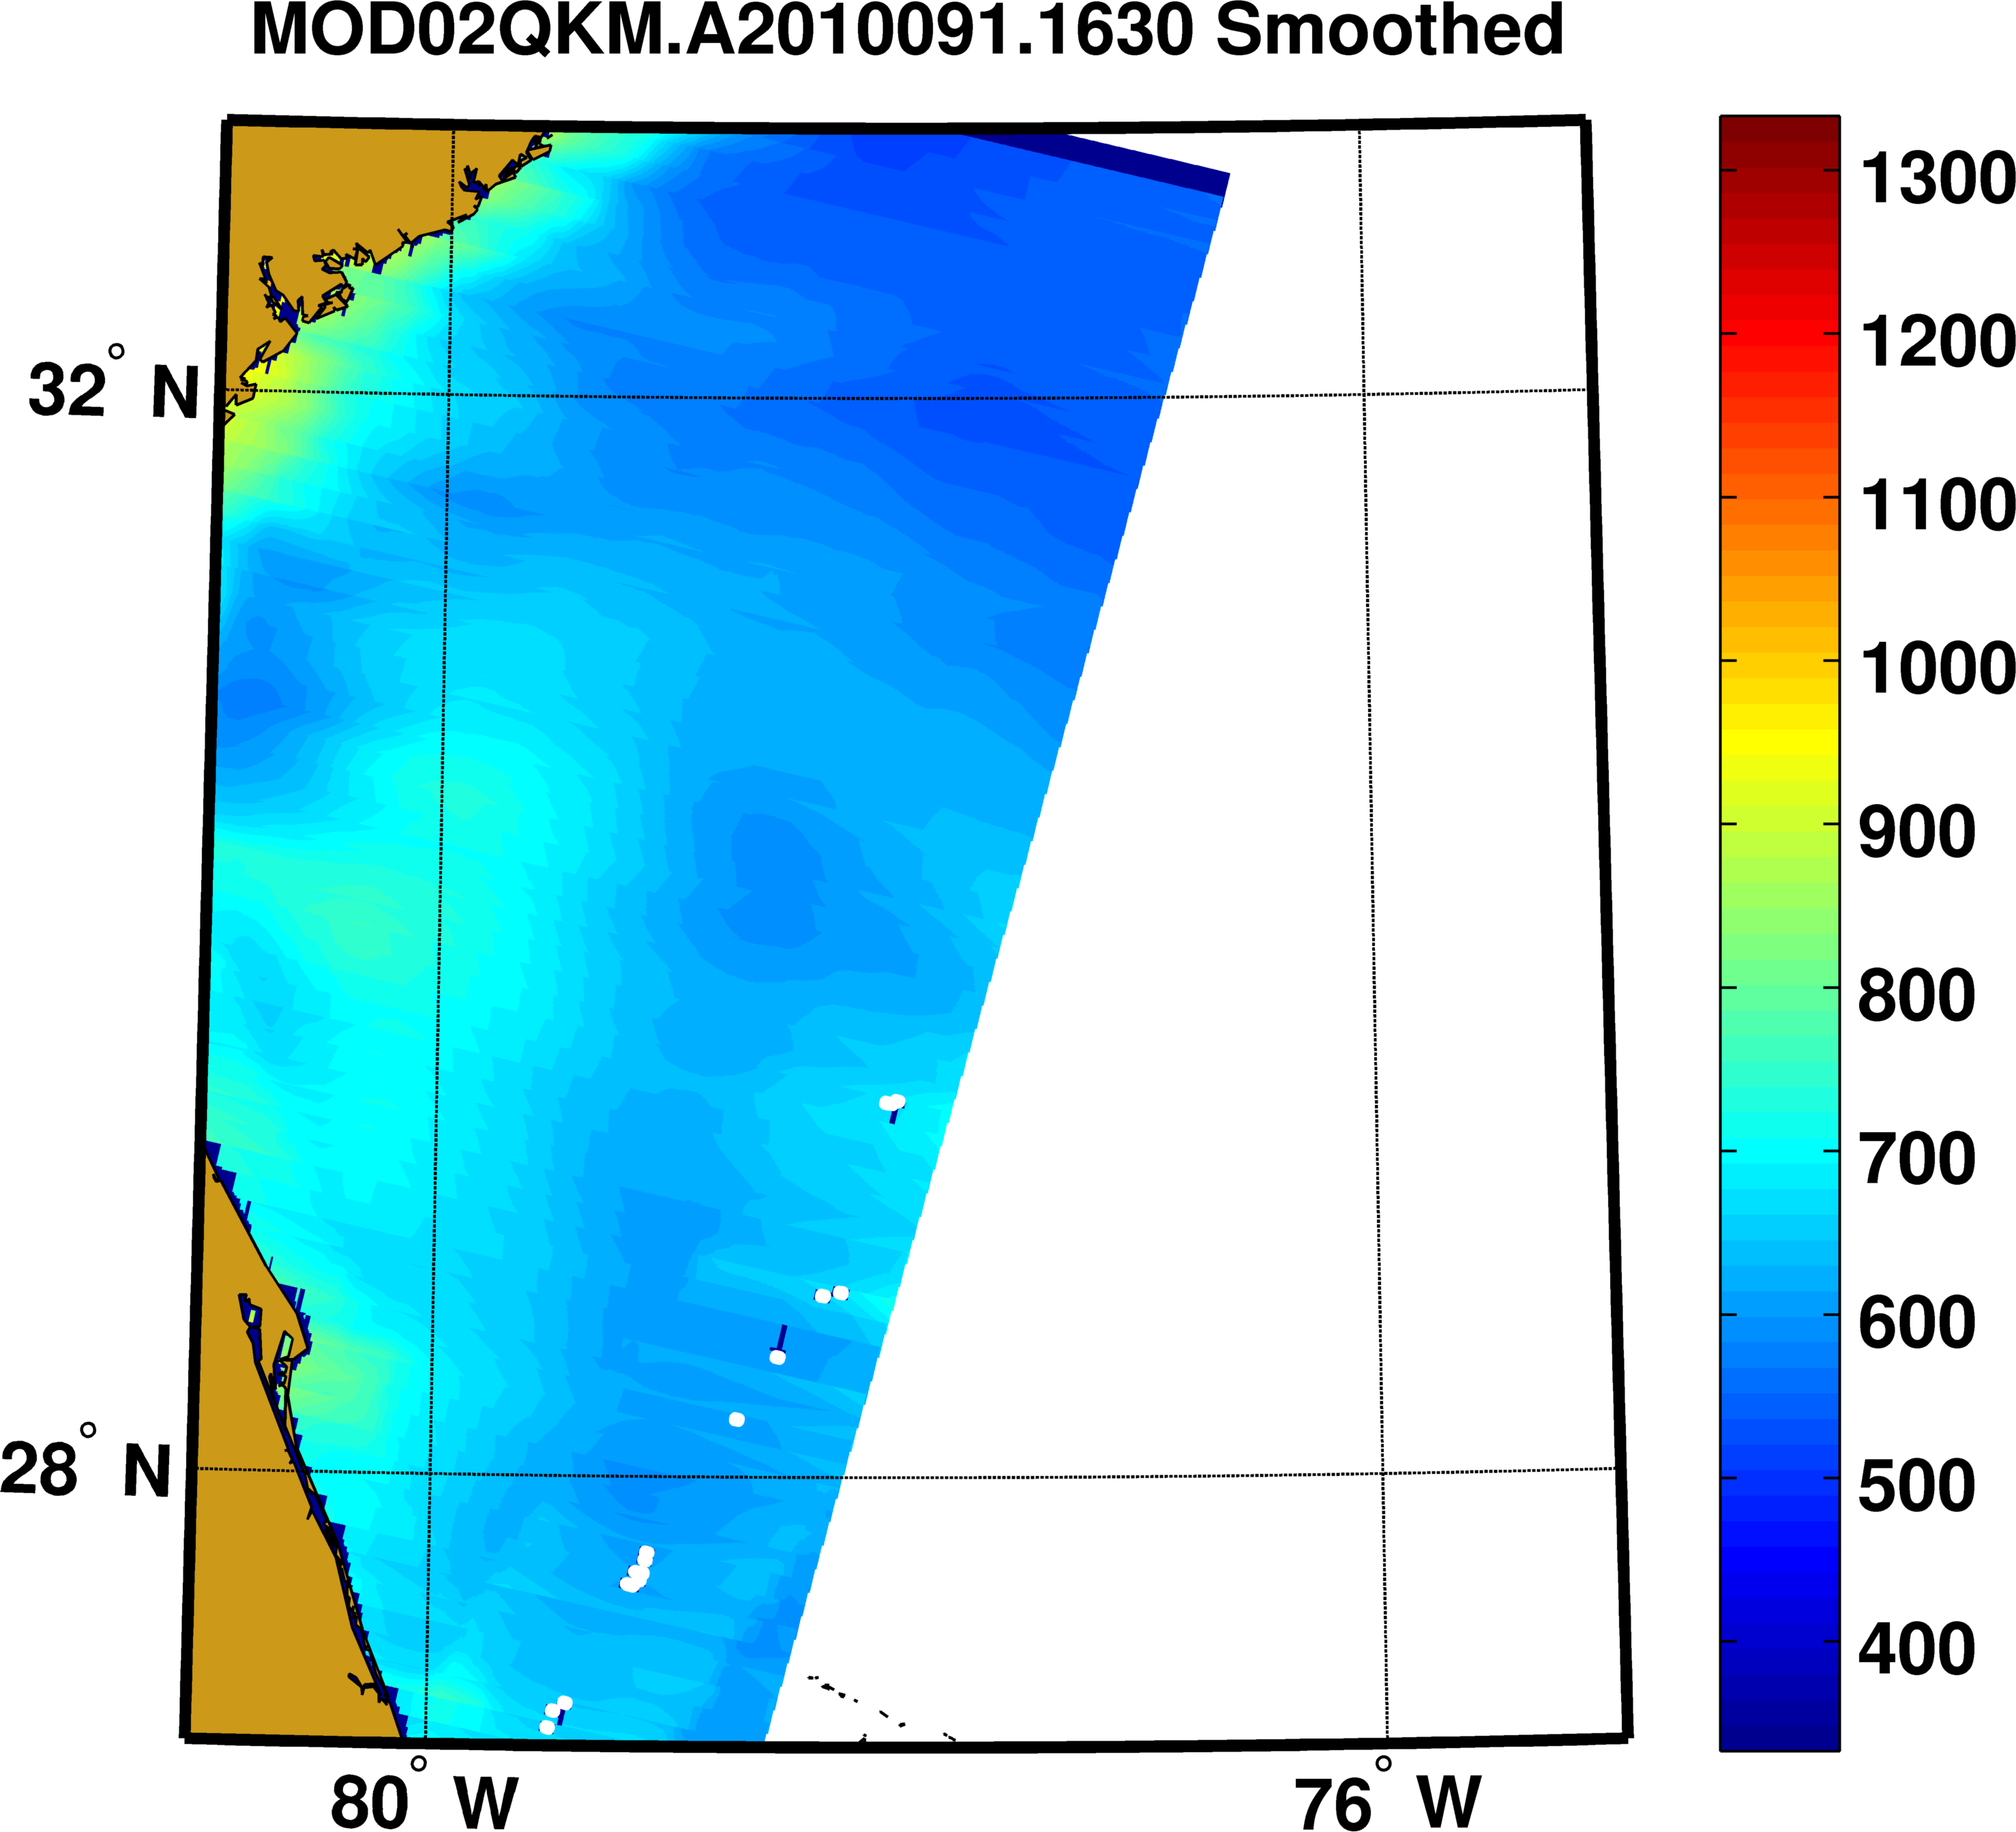
\includegraphics[width=1\linewidth]{fig14b}}
	\end{minipage}
	\hfill
	\begin{minipage}{.31\textwidth}
	    \subcaptionbox{\label{fig:14c}}
		{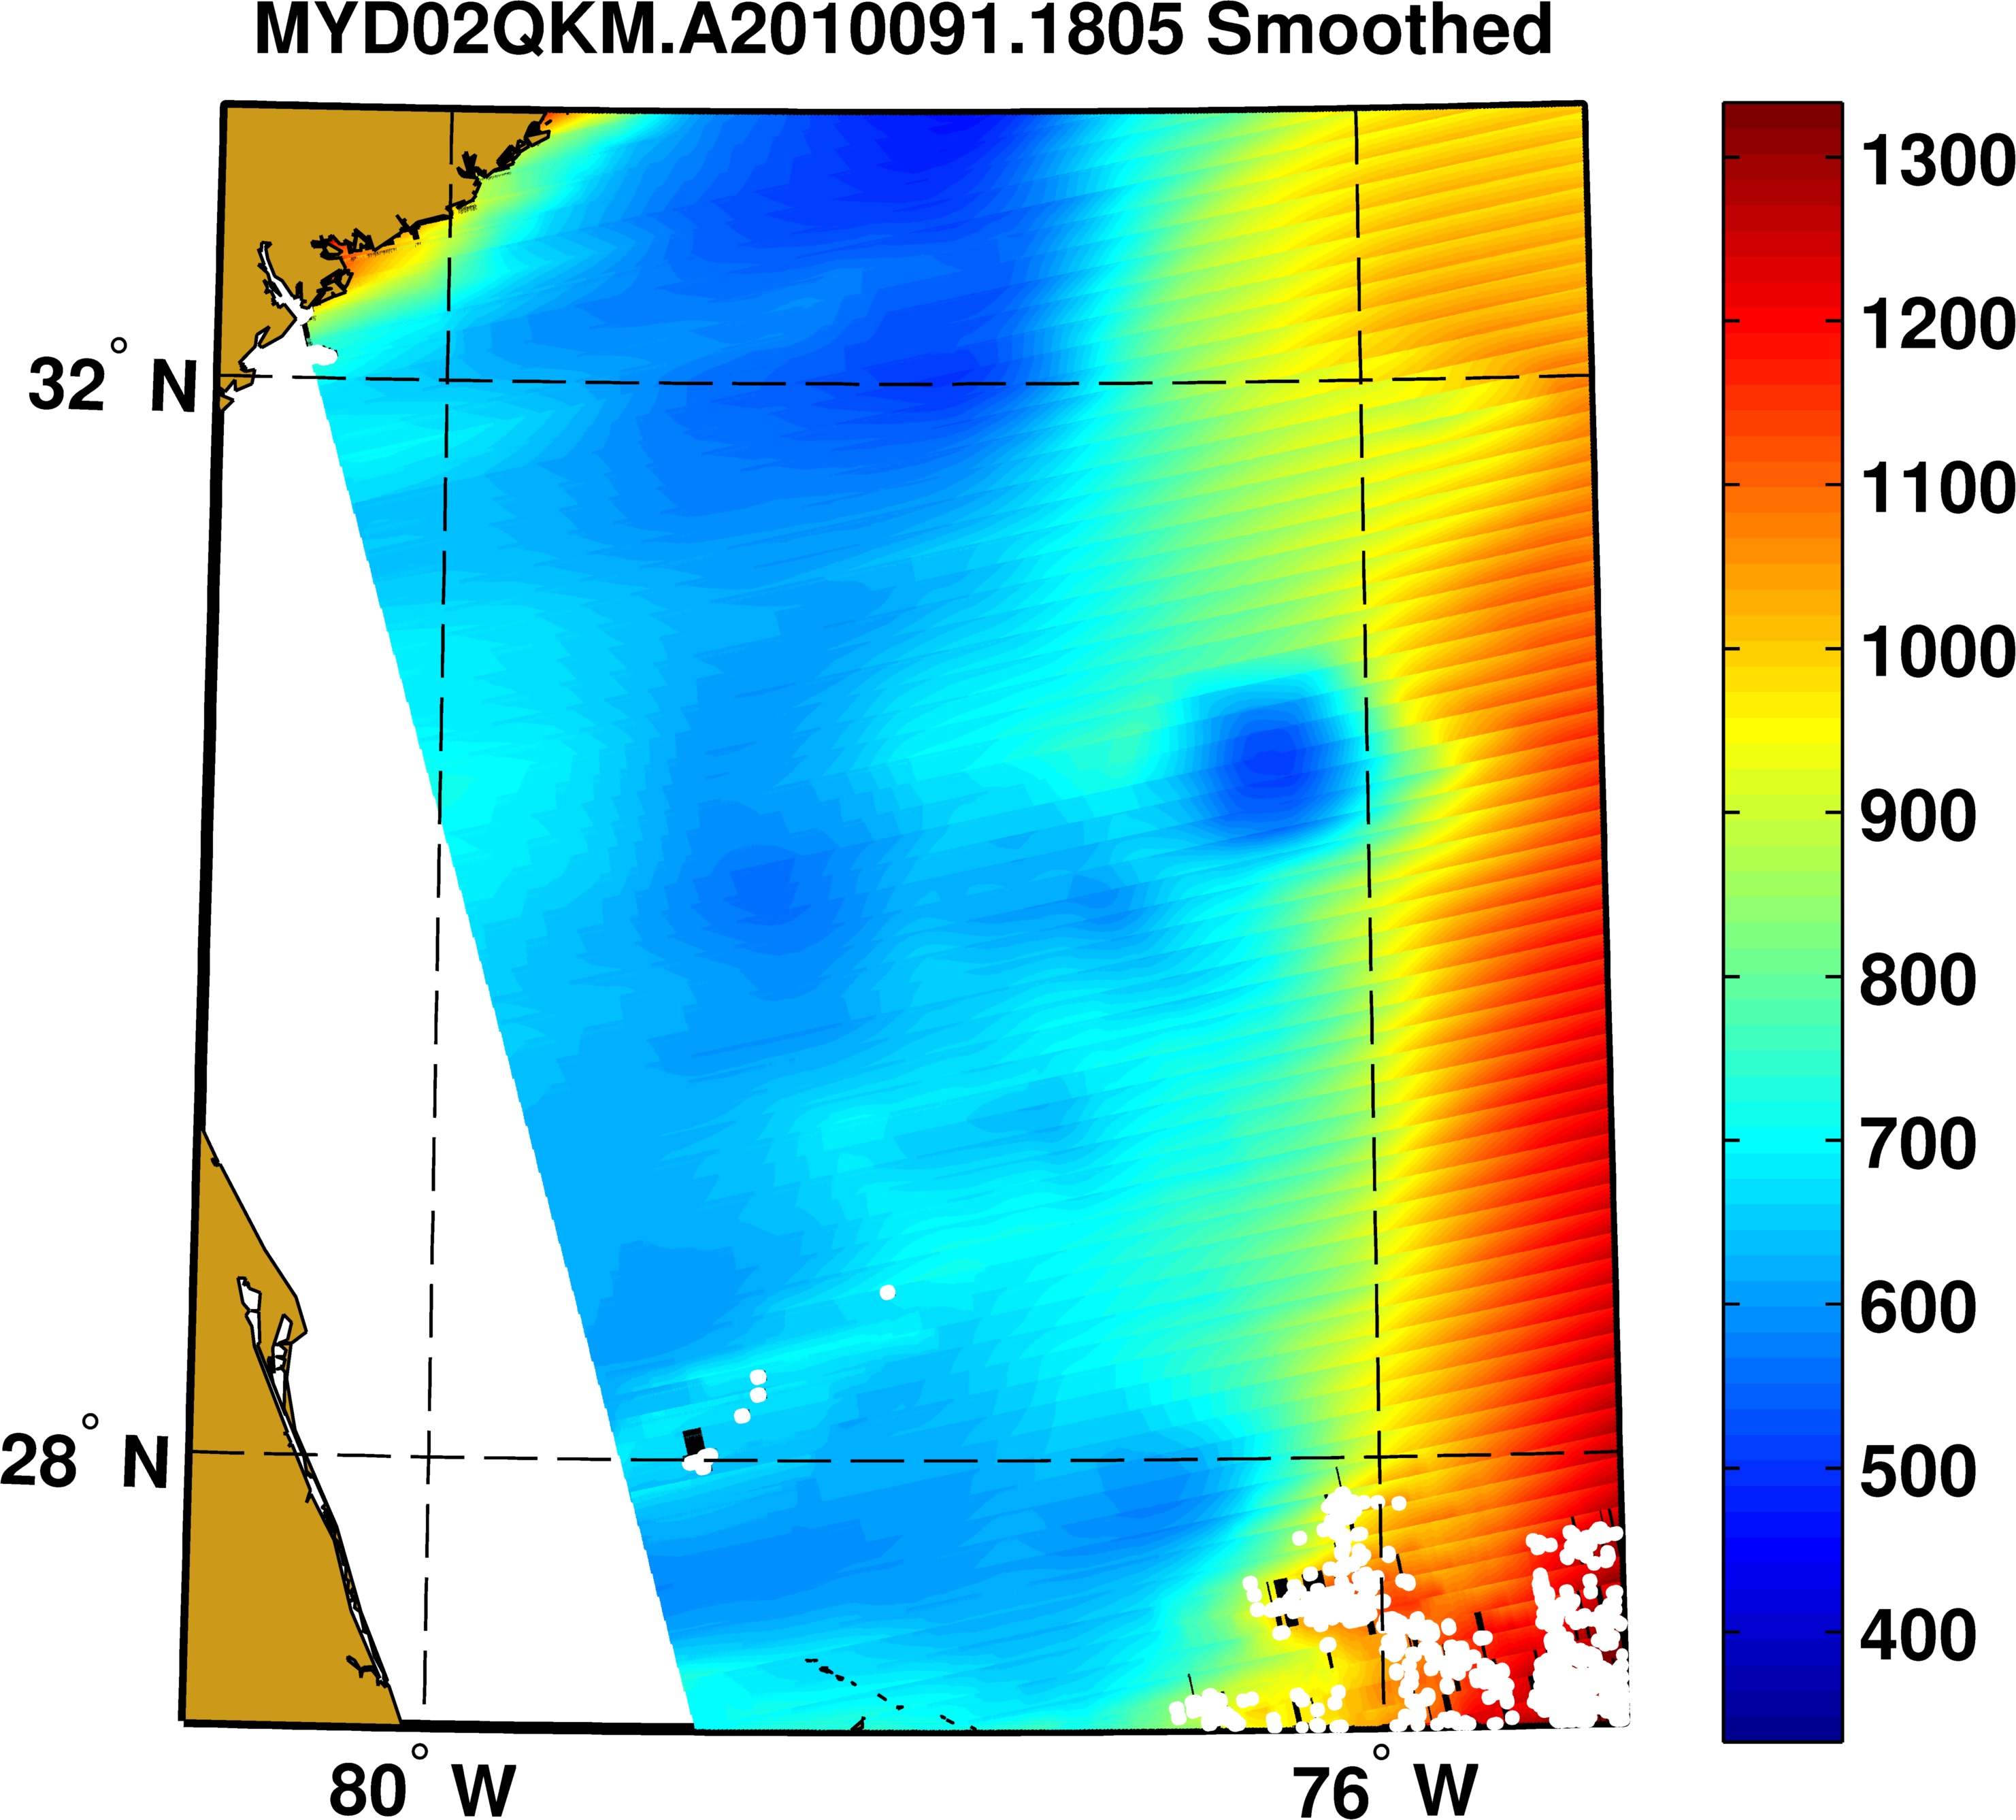
\includegraphics[width=1\linewidth]{fig14c}}
	\end{minipage}
	\\
    \floattitle{MERIS (а), MODIS/Terra (б) и MODIS/Aqua (в)}
    \caption{Средняя яркость солнечного блика (масштаб осреднения 30x30км${}^2$)}
    \label{fig:14}
\end{figure}




Контрасты яркости солнечного блика $\tilde{B}/B_{0}$, получаемые после устранения эффекта ``пилы'', представлены на Рисунке~\ref{fig:15}.



\begin{figure}[H]
    	\centering
	\begin{minipage}{.31\textwidth}
	    \subcaptionbox{\label{fig:15a}}
		{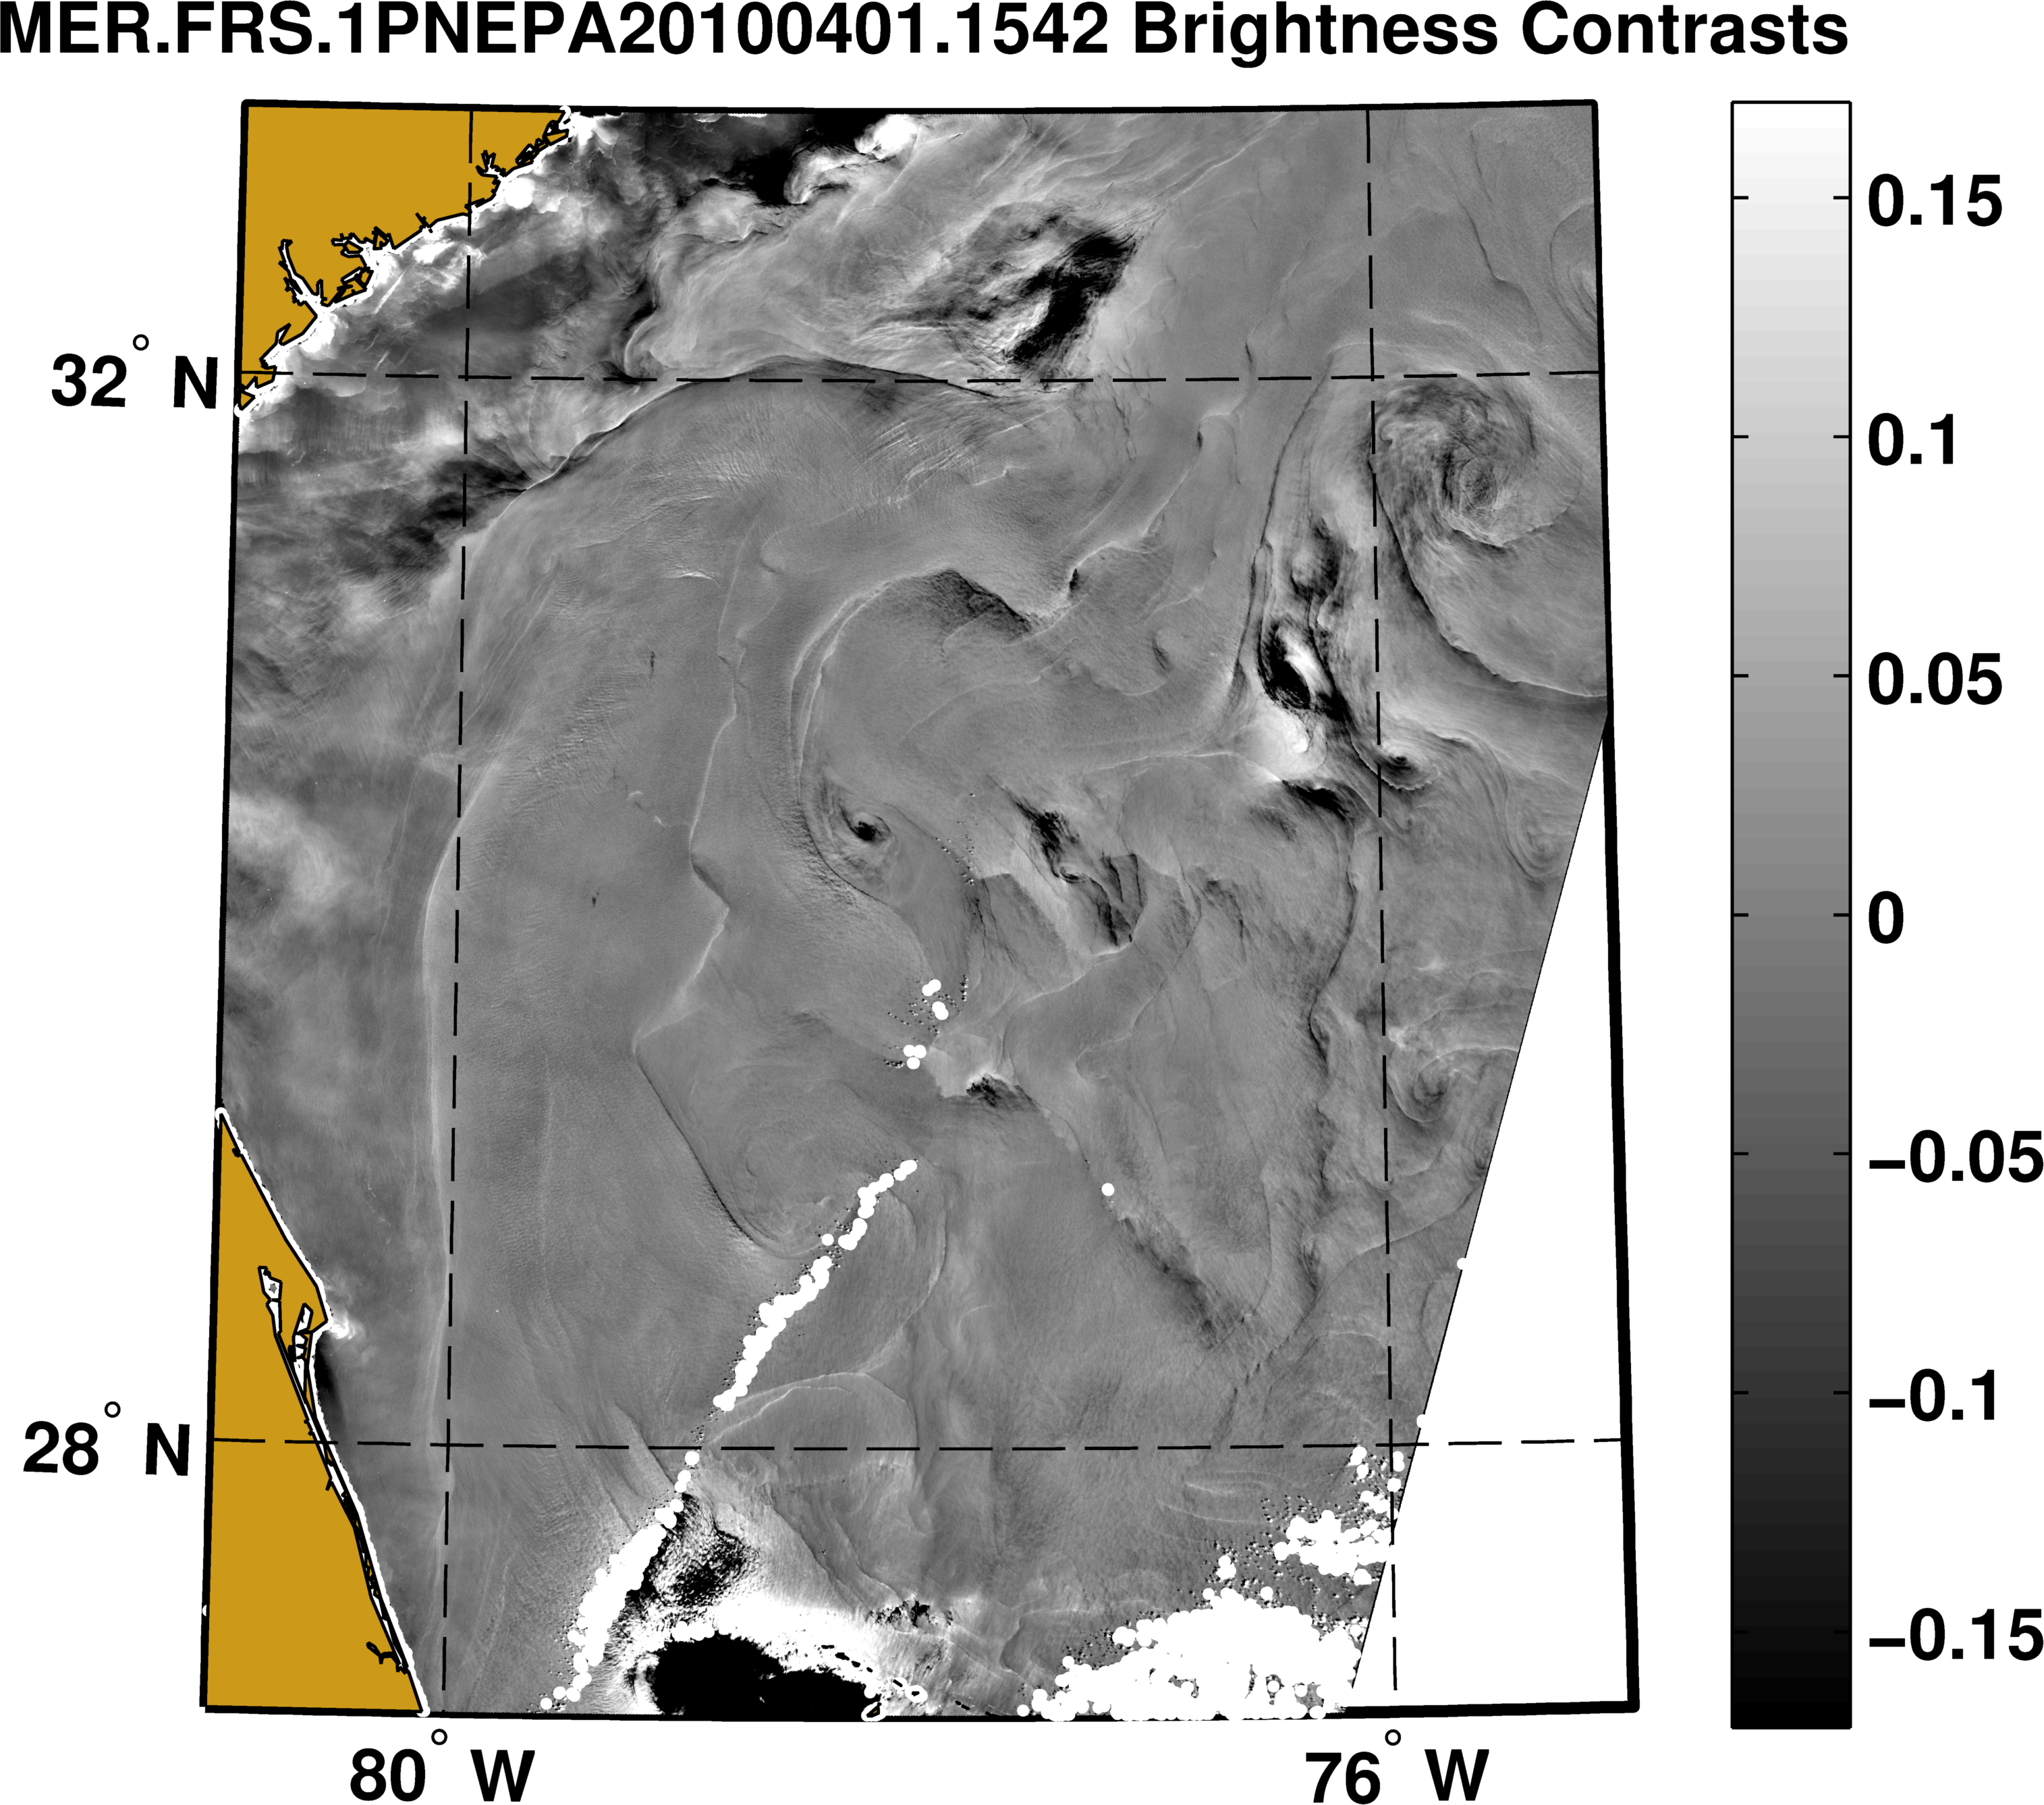
\includegraphics[width=1\linewidth]{fig15a}}
	\end{minipage}
	\hfill
	\begin{minipage}{.31\textwidth}
	    \subcaptionbox{\label{fig:15b}}
		{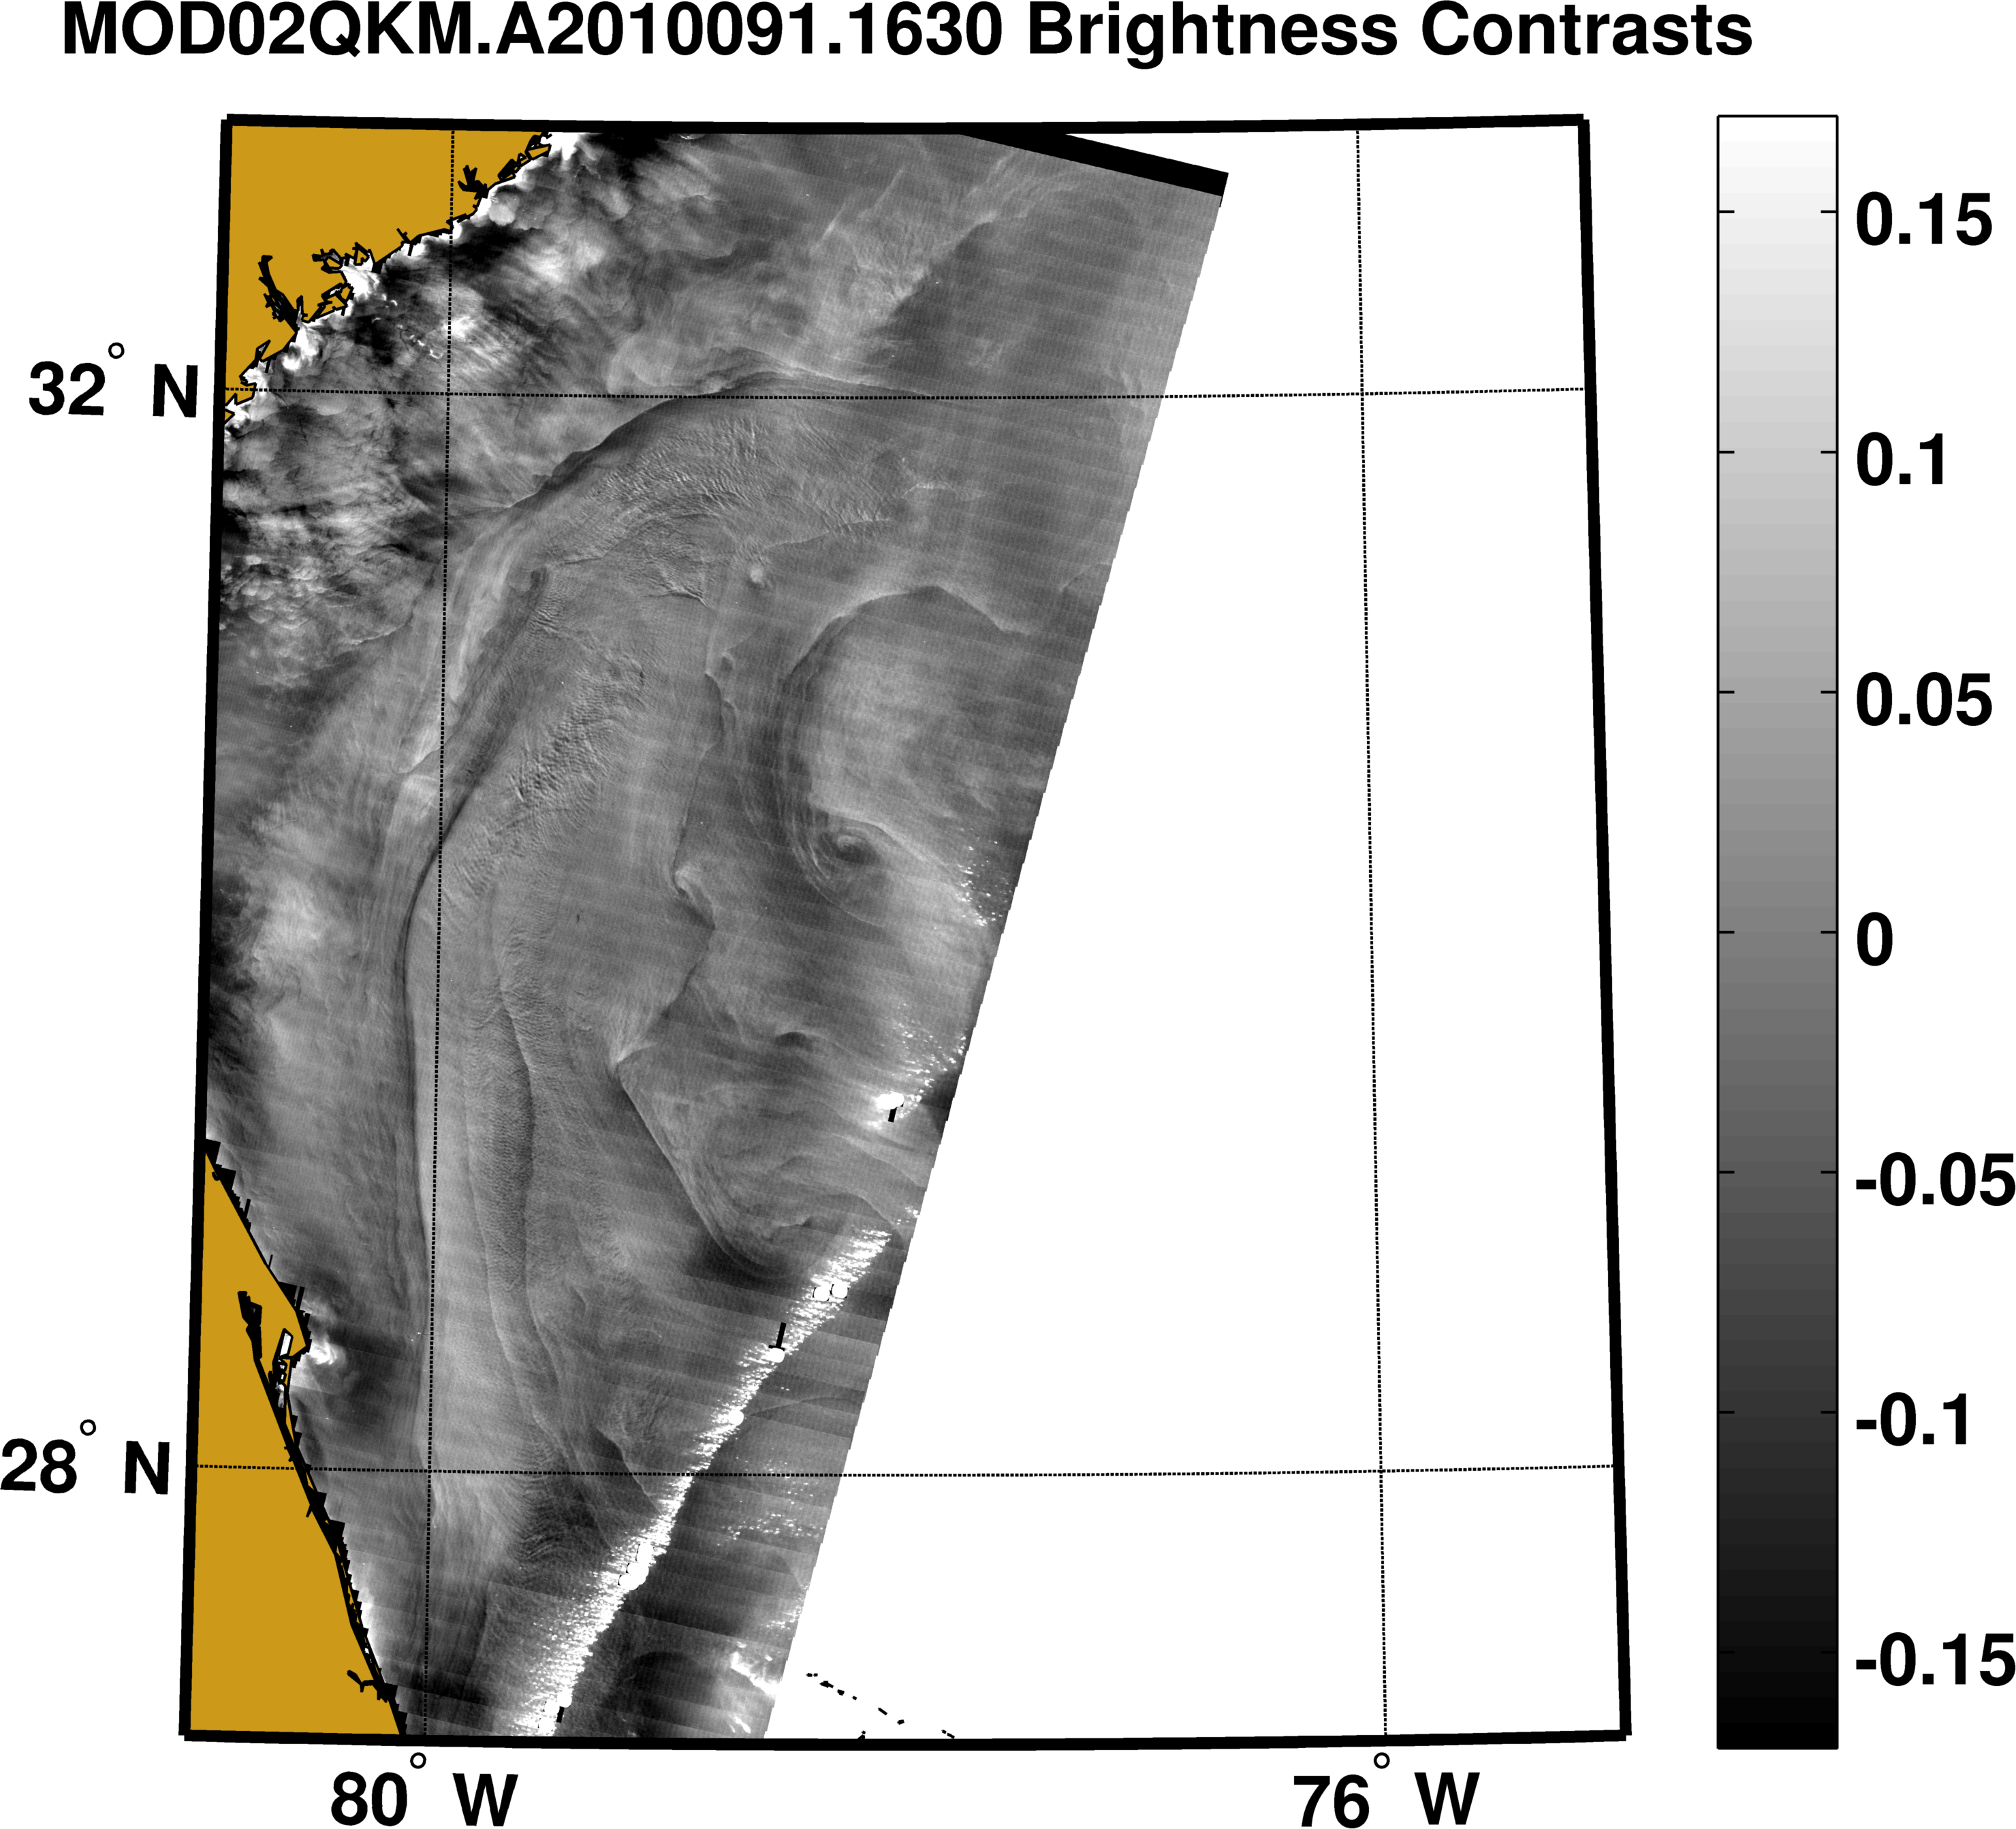
\includegraphics[width=1\linewidth]{fig15b}}
	\end{minipage}
	\hfill
	\begin{minipage}{.31\textwidth}
	    \subcaptionbox{\label{fig:15c}}
		{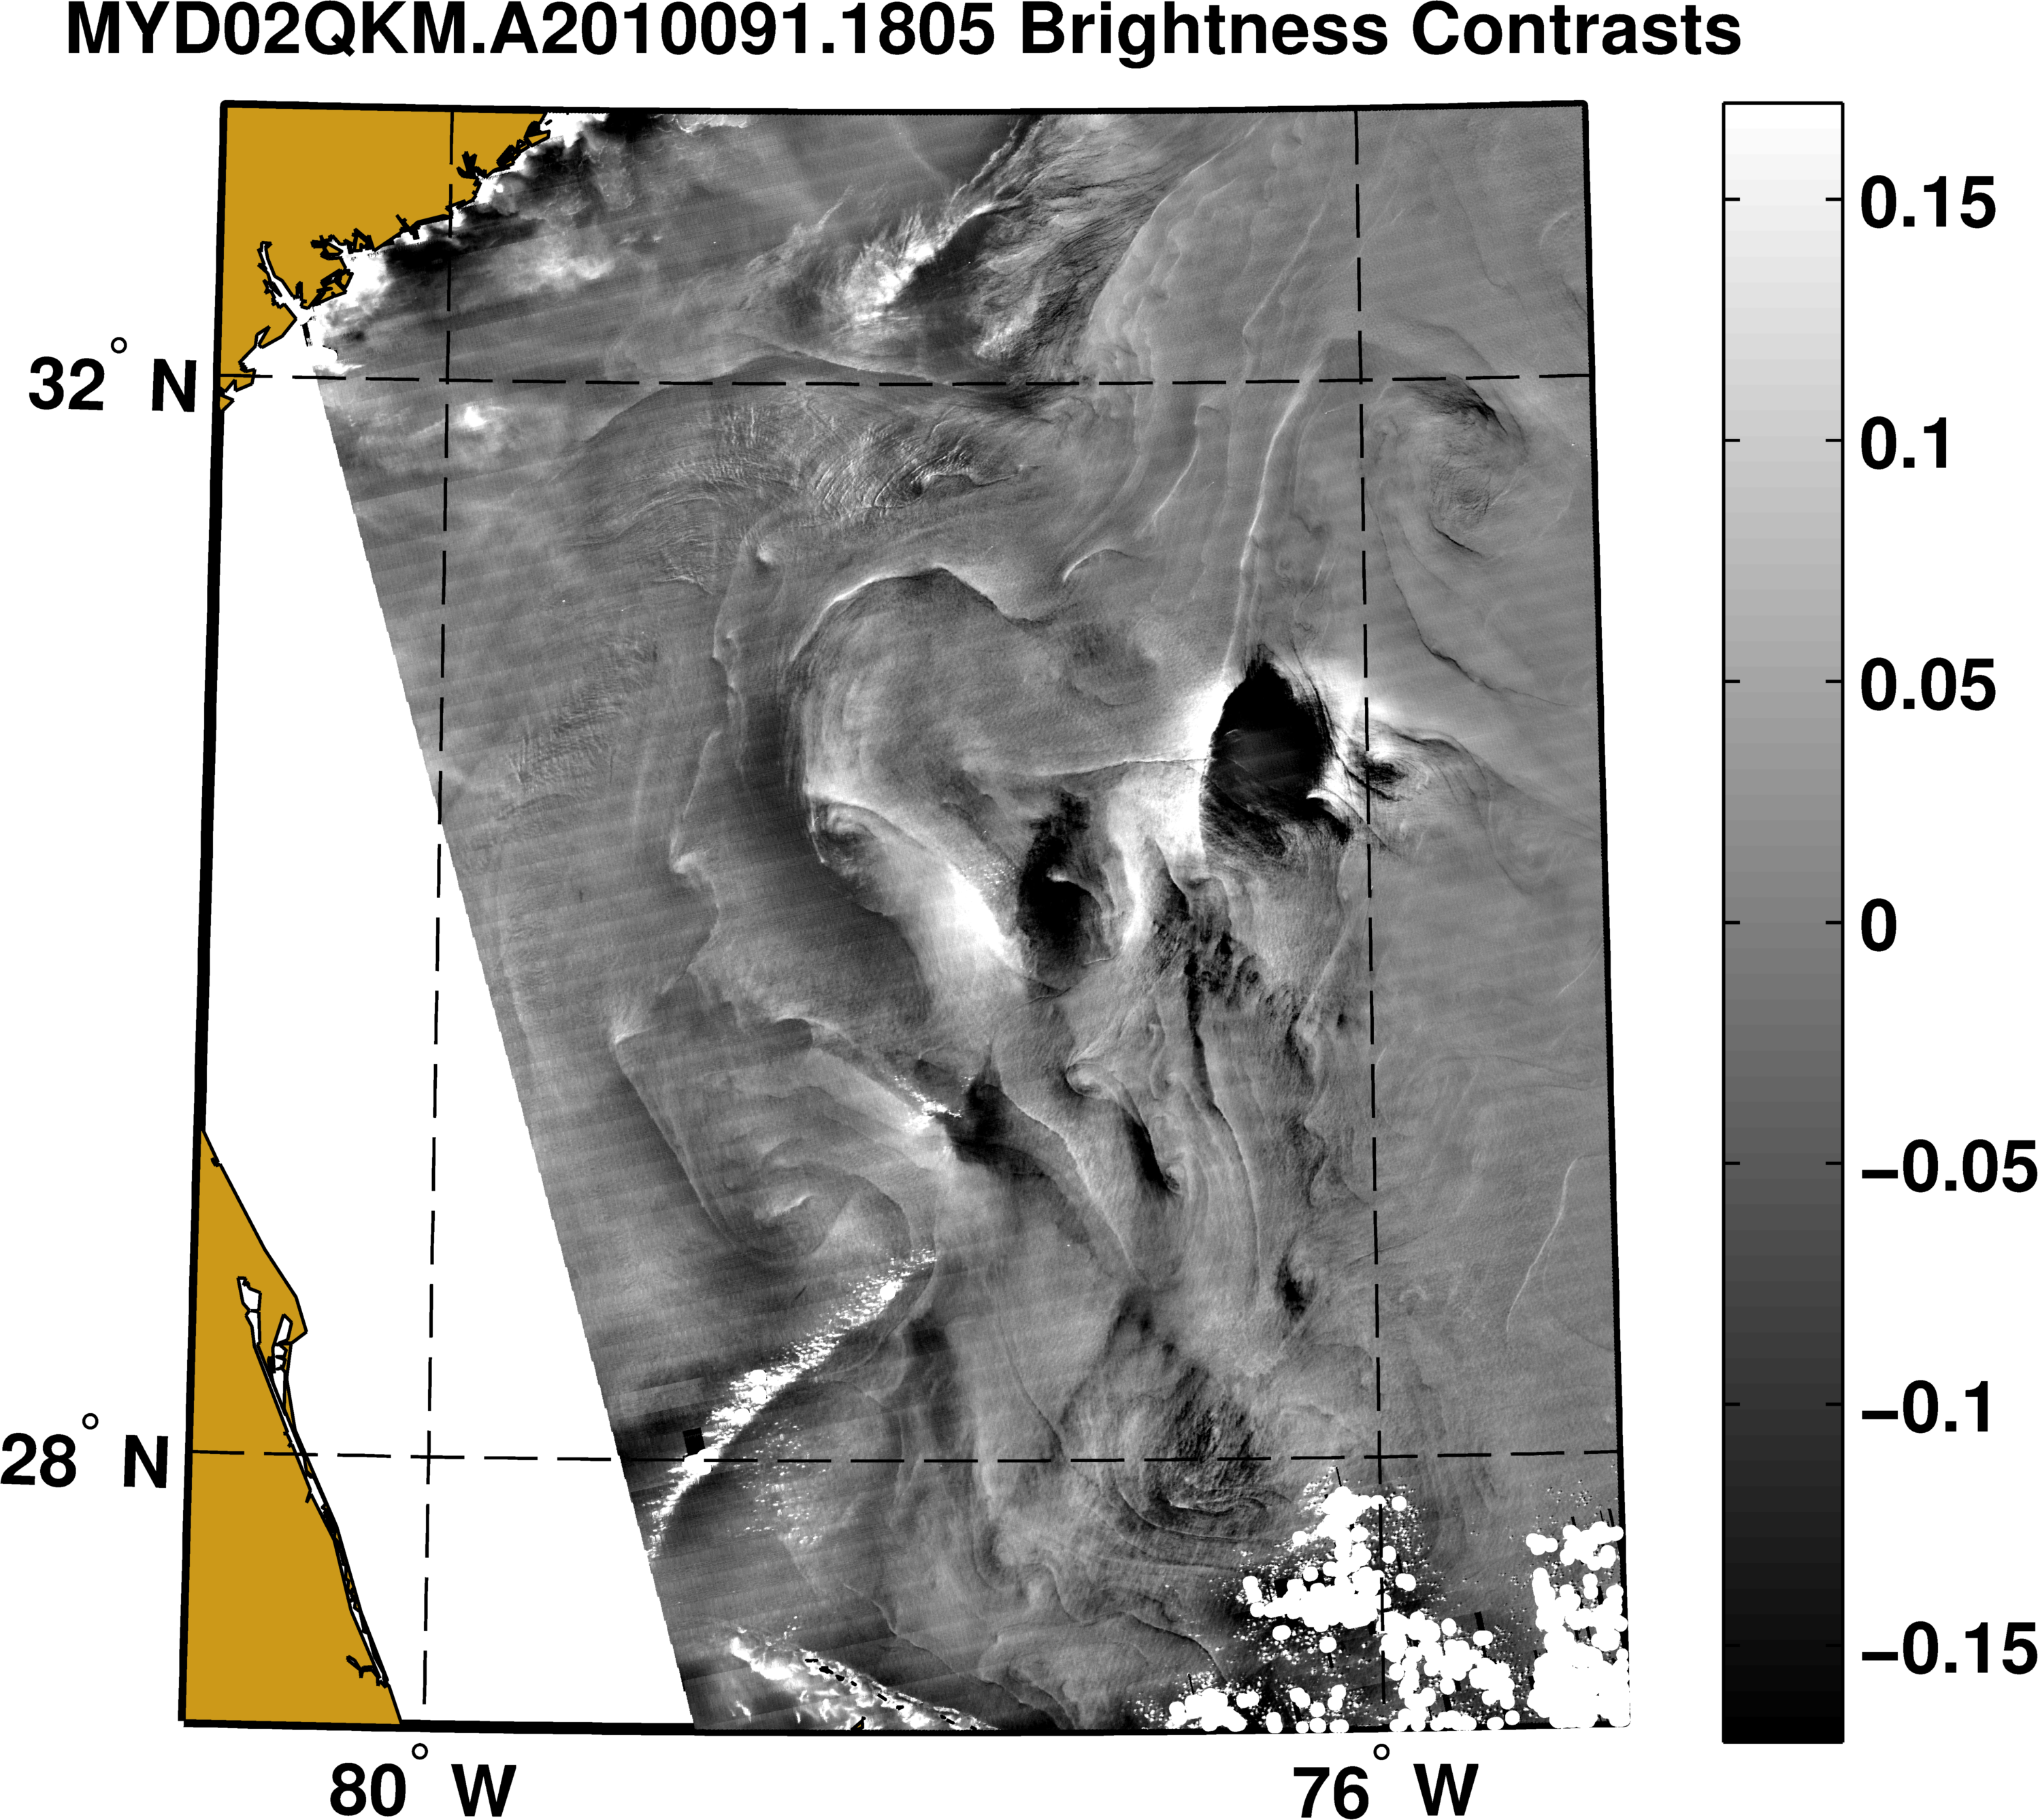
\includegraphics[width=1\linewidth]{fig15c}}
	\end{minipage}
	\\
    \floattitle{MERIS (а), MODIS/Terra (б) и MODIS/Aqua (в)}
    \caption{Контрасты яркости солнечного блика $\tilde{B}/B_{0}$}
    \label{fig:15}
\end{figure}



Передаточная функция, рассчитанная по уравнению \eqref{eq:1.7}, для сглаженного поля яркости солнечного блика изображена на Рисунке~\ref{fig:16}. При рассмотрении изображений передаточной функции можно заметить, что поле, полученное по данным MERIS, более однородно и в большей степени напоминает эллипс (Рисунок~\ref{fig:16a}), нежели на изображениях передаточной функции MODIS (Рисунки~\ref{fig:16b}, \ref{fig:16c}). Объяснить наблюдаемое возможно, если обратиться к геометрии наблюдений. На Рисунках~\ref{fig:17} и \ref{fig:18} представлены карты локальных наклонов поверхности, обеспечивающих зеркальное отражение и карты зон инверсии контрастов, соответственно. Обратимся сначала к рассмотрению локальных наклонов поверхности.


\begin{figure}[H]
    	\centering
	\begin{minipage}{.33\textwidth}
	    \subcaptionbox{\label{fig:16a}}
		{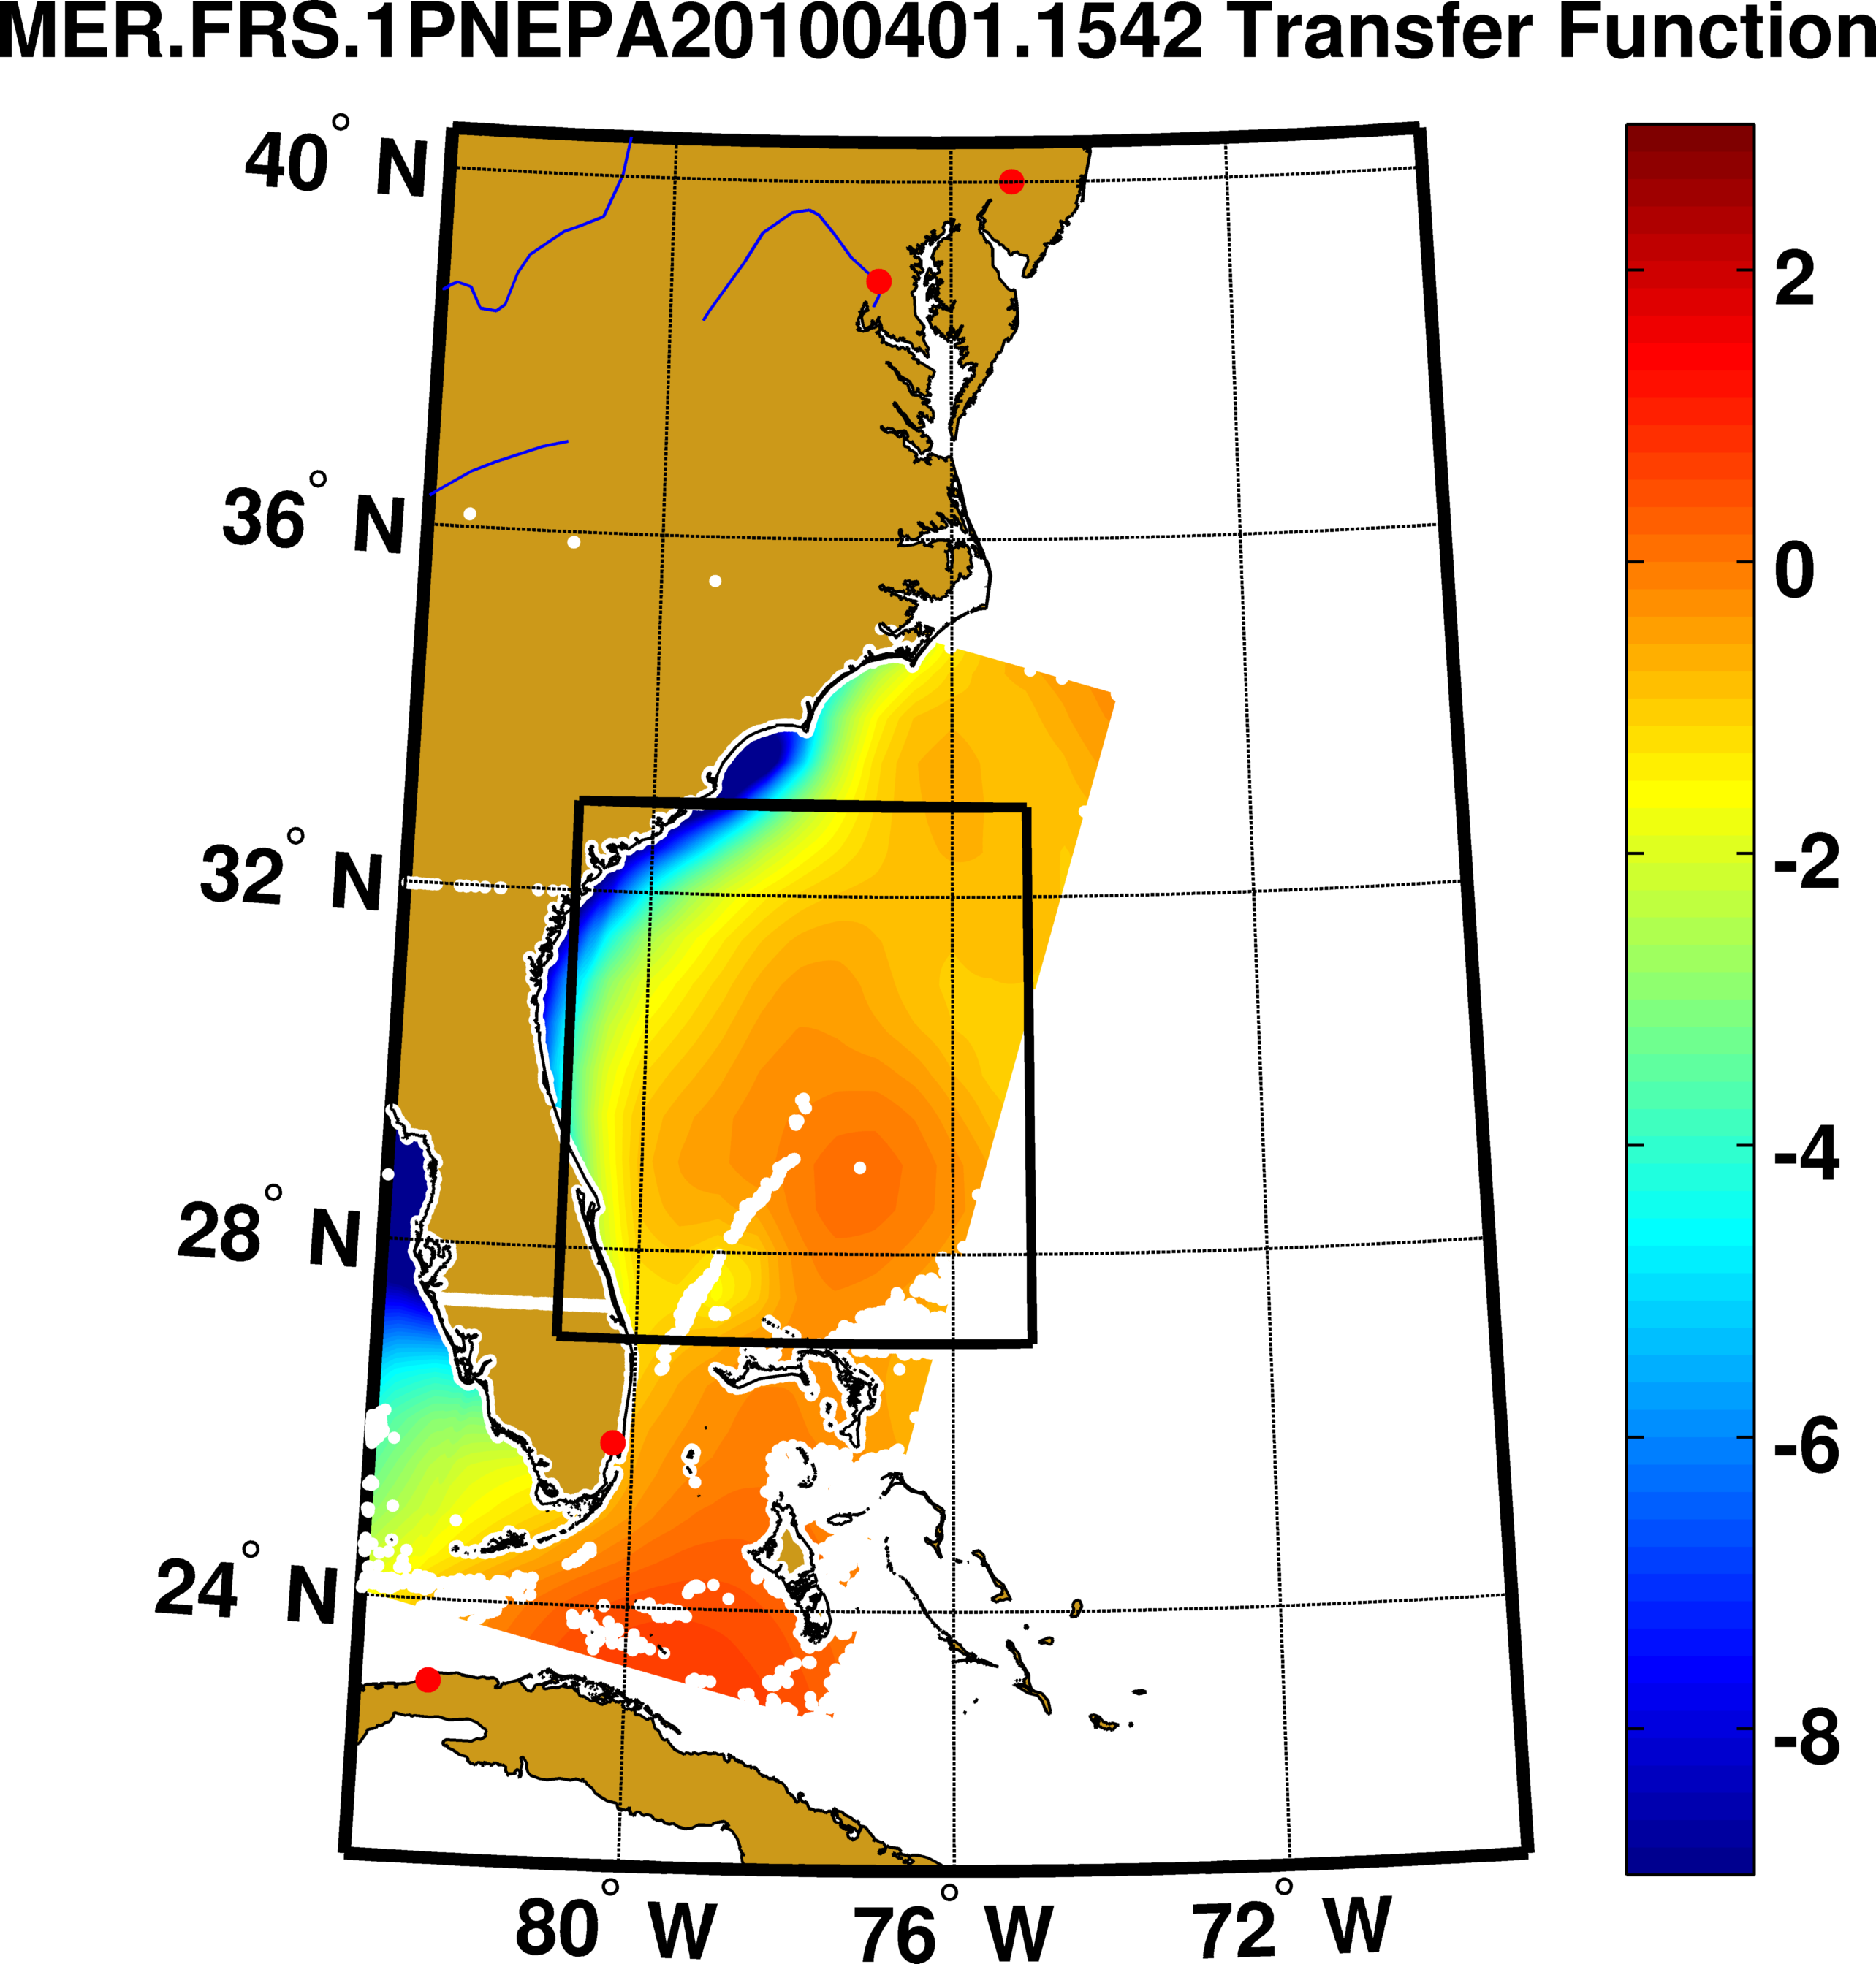
\includegraphics[width=1\linewidth]{fig16a}}
	\end{minipage}
	\hfill
	\begin{minipage}{.31\textwidth}
	    \subcaptionbox{\label{fig:16b}}
		{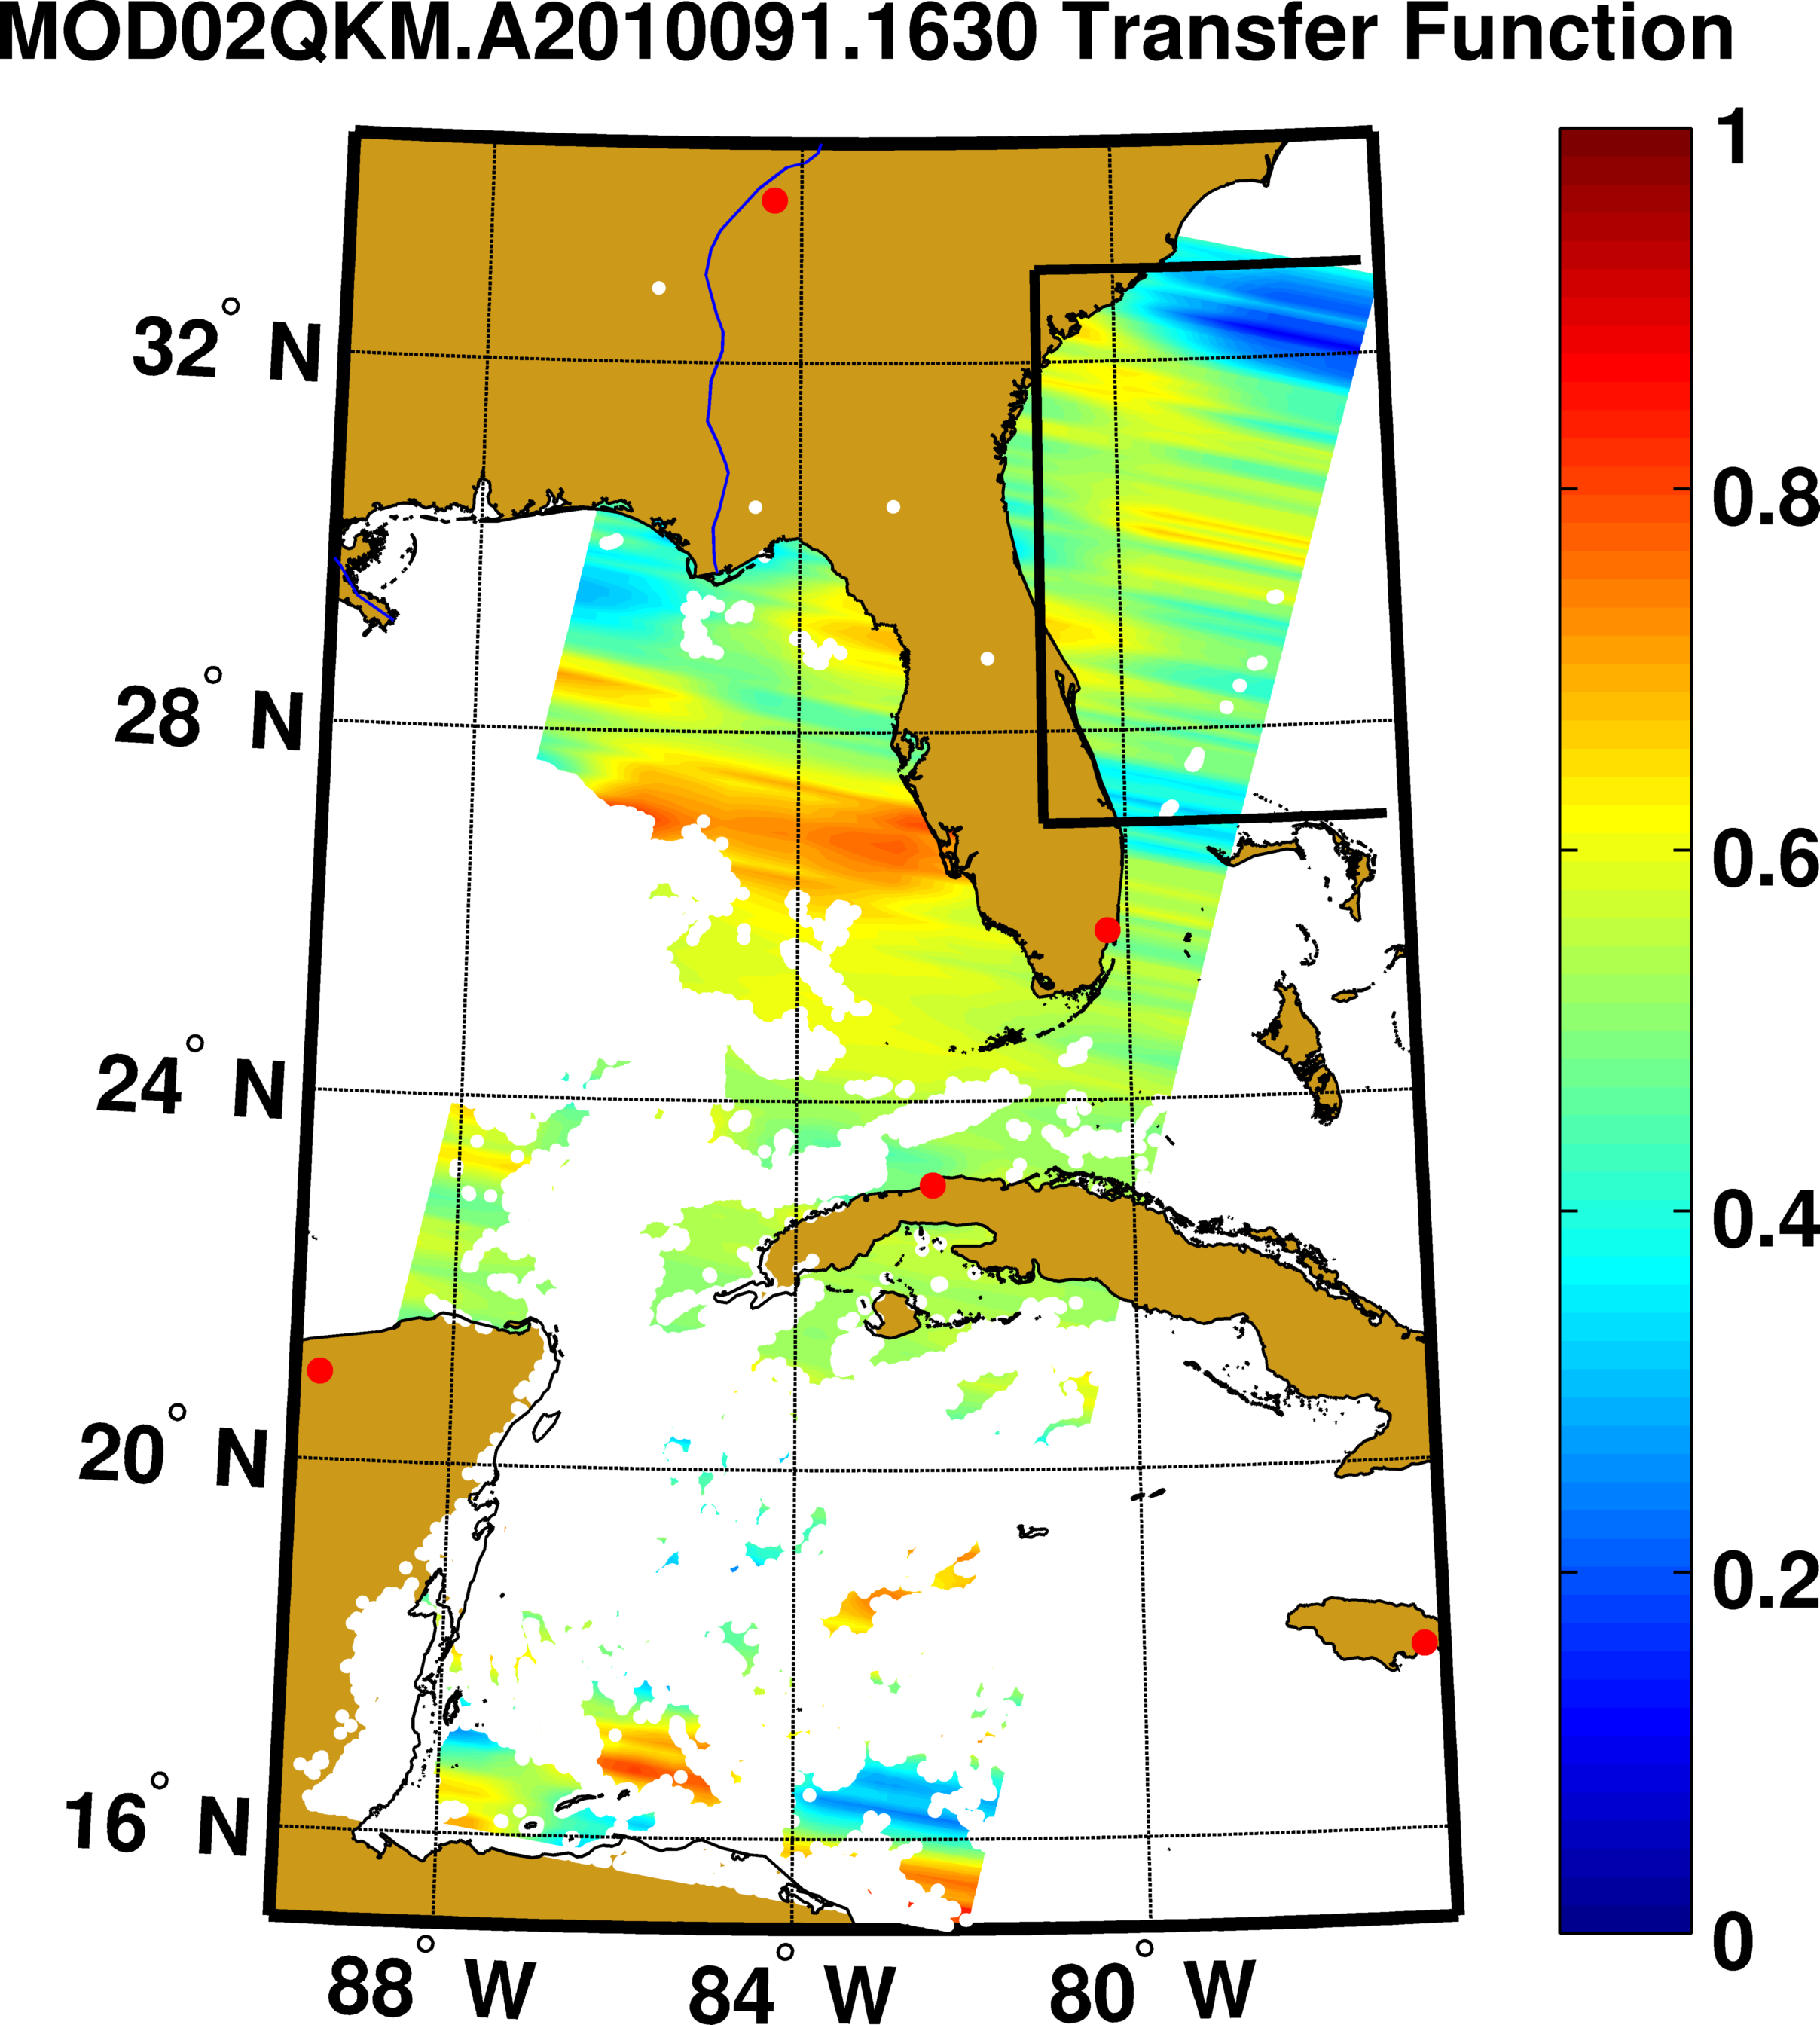
\includegraphics[width=1\linewidth]{fig16b}}
	\end{minipage}
	\hfill
	\begin{minipage}{.31\textwidth}
	    \subcaptionbox{\label{fig:16c}}
		{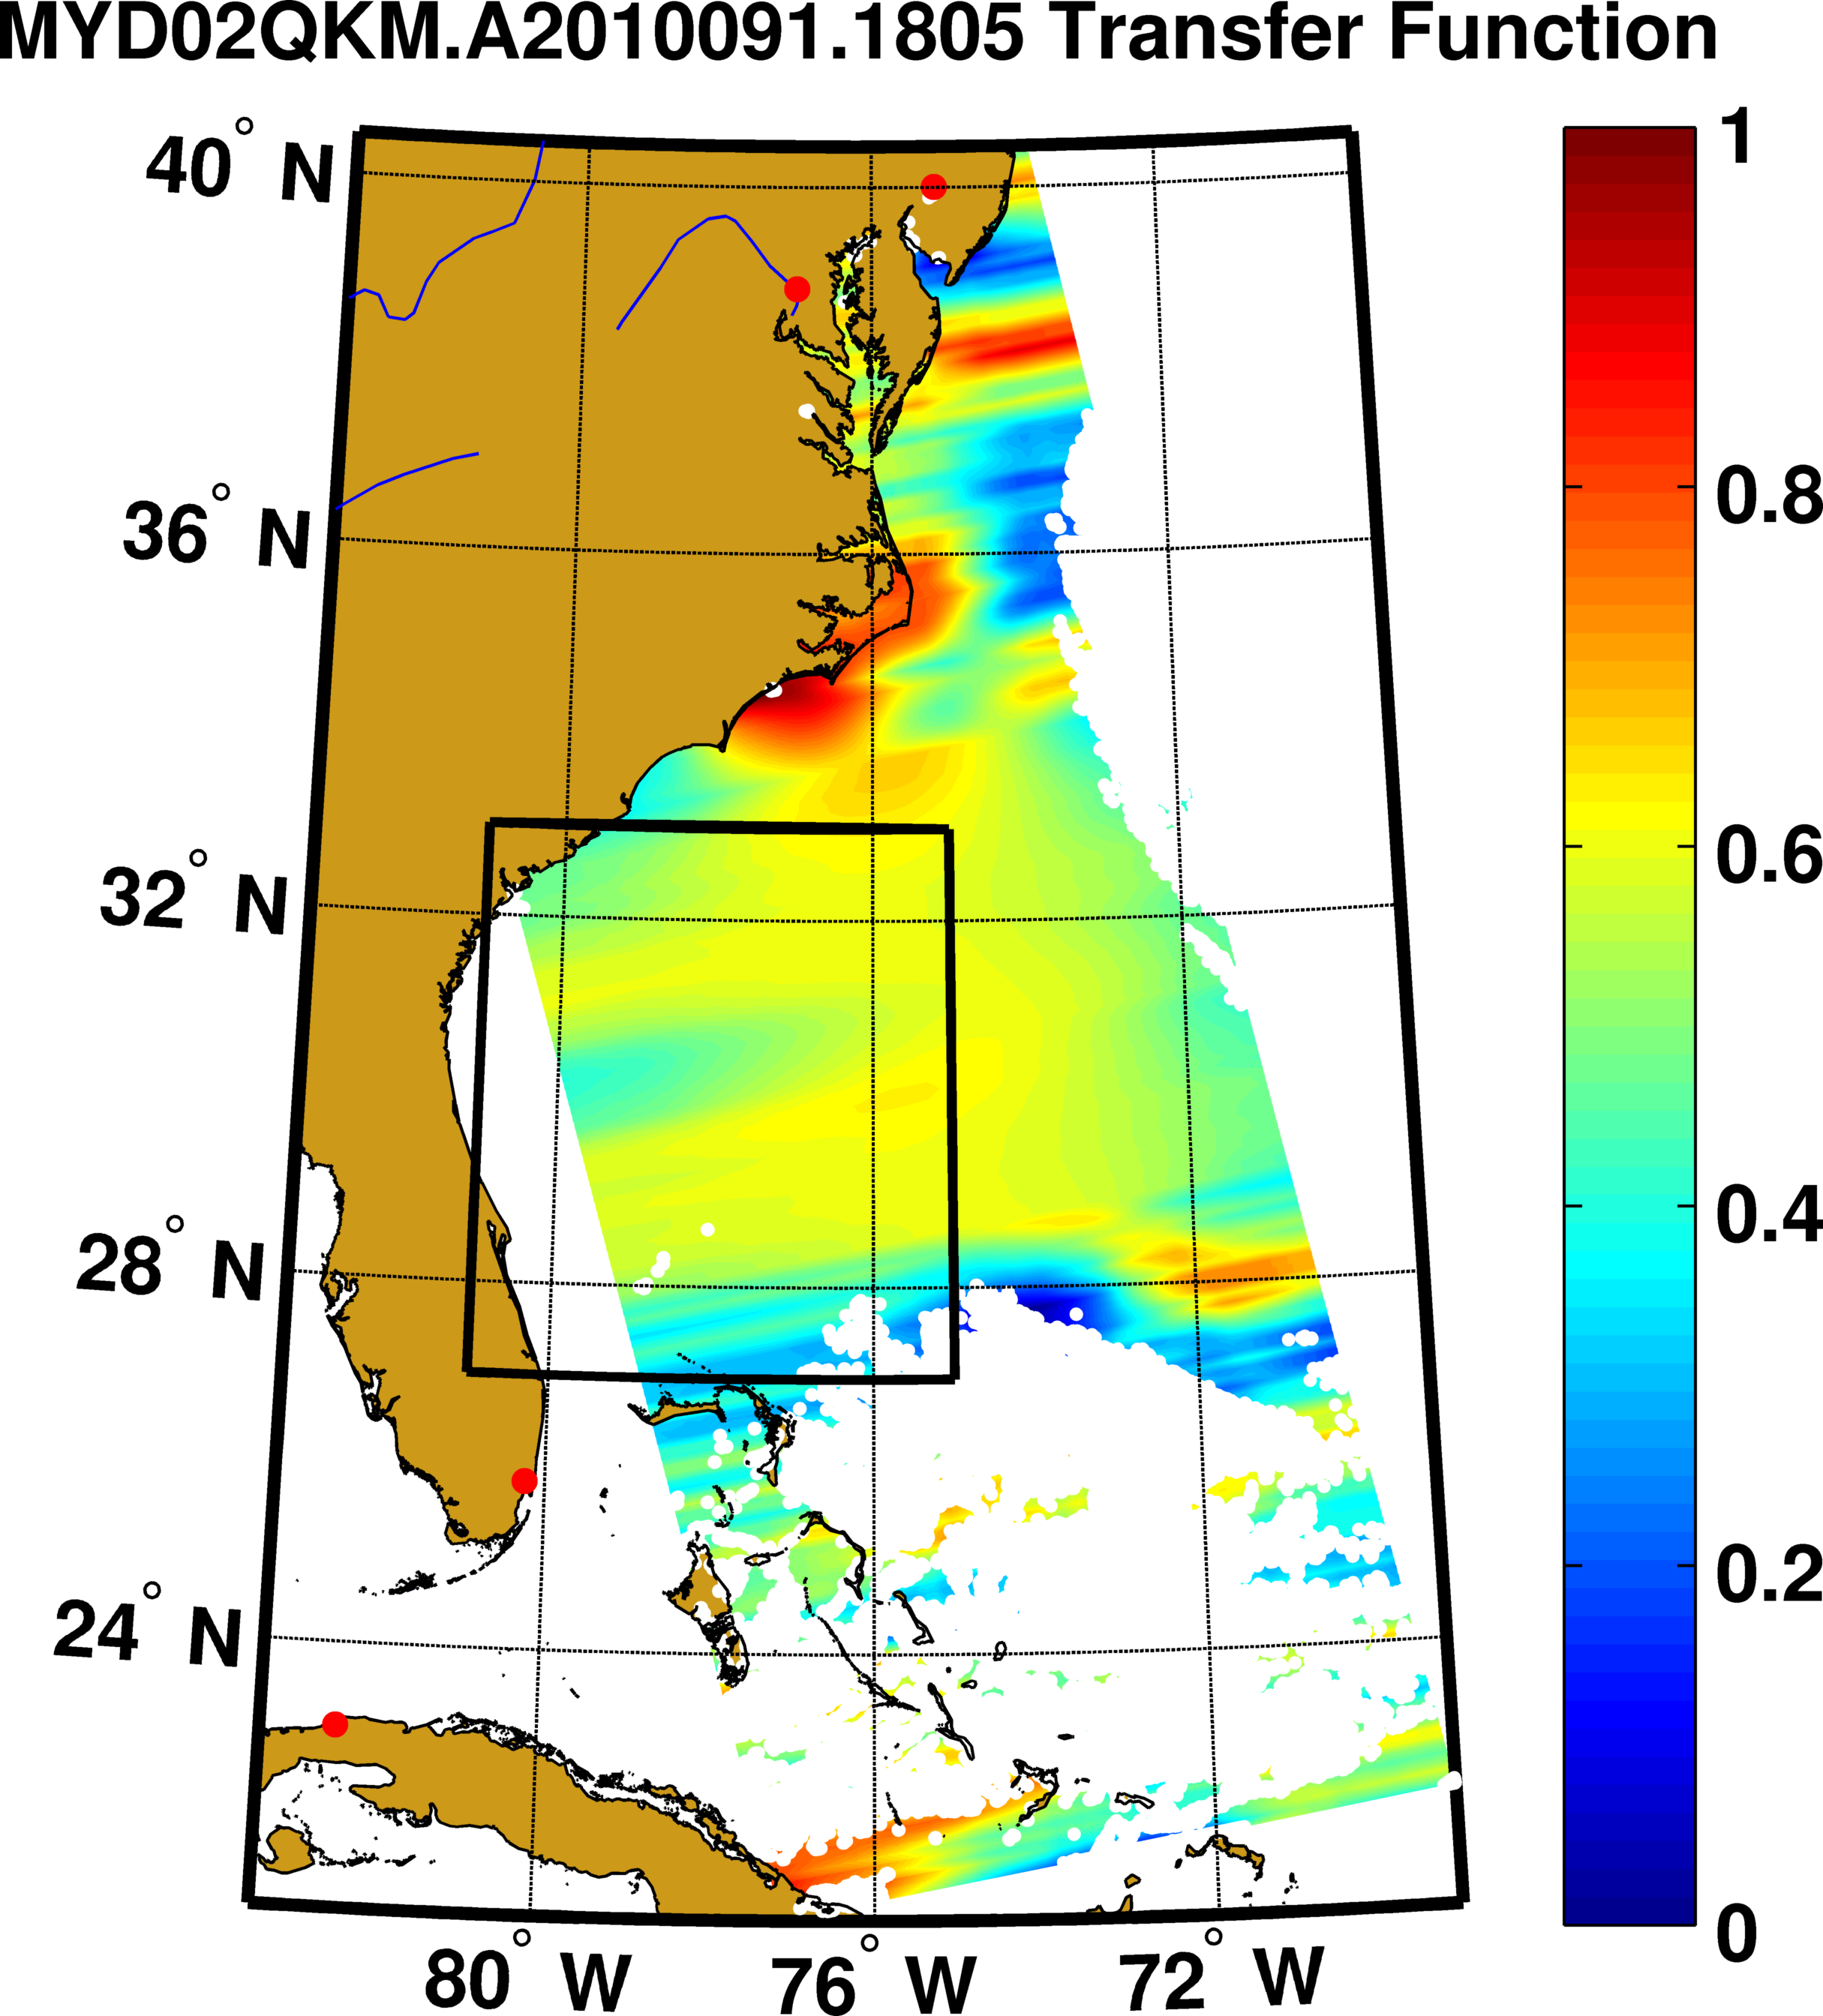
\includegraphics[width=1\linewidth]{fig16c}}
	\end{minipage}
	\\
    \floattitle{MERIS (а), MODIS/Terra (б) и MODIS/Aqua (в)}
    \caption{Передаточная функция  для связи контрастов вариаций яркости (Рисунок~\ref{fig:15}) и контрастов СКН (Рисунок~\ref{fig:16})}
    \label{fig:16}
\end{figure}




\begin{figure}[H]
    	\centering
	\begin{minipage}{.33\textwidth}
	    \subcaptionbox{\label{fig:17a}}
		{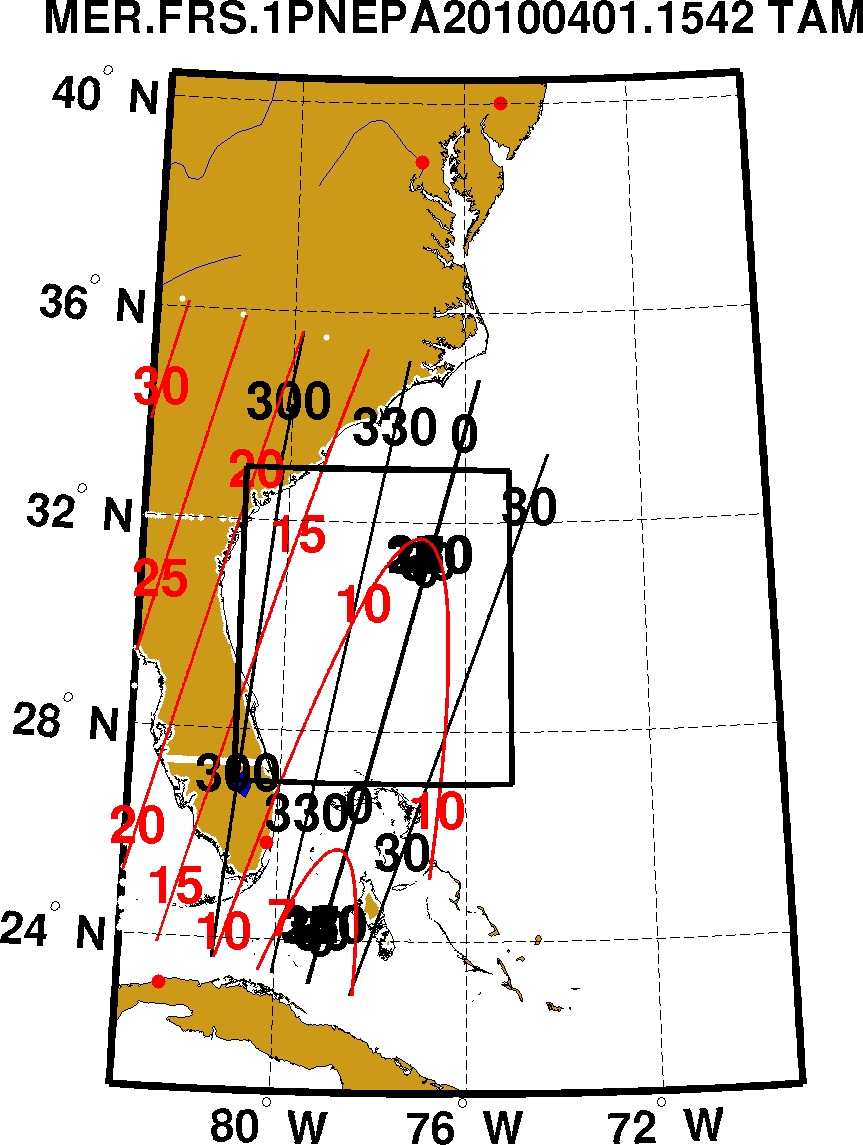
\includegraphics[width=1\linewidth]{fig17a}}
	\end{minipage}
	\hfill
	\begin{minipage}{.31\textwidth}
	    \subcaptionbox{\label{fig:17b}}
		{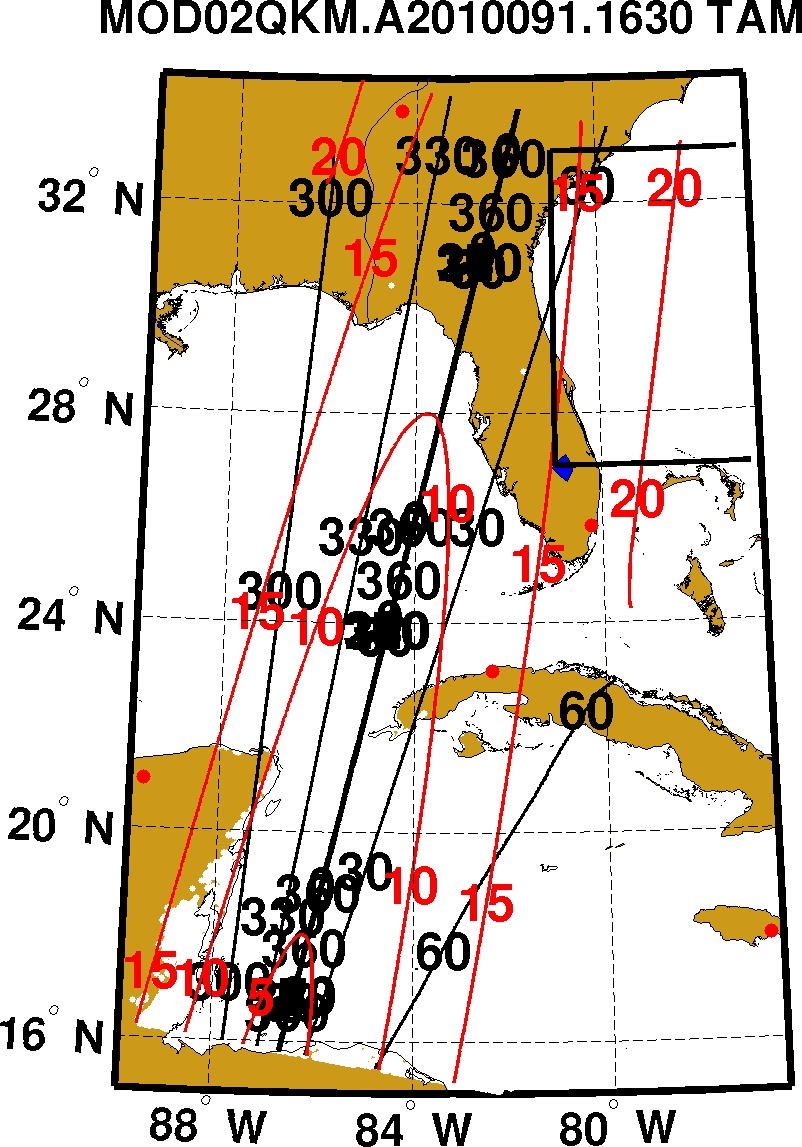
\includegraphics[width=1\linewidth]{fig17b}}
	\end{minipage}
	\hfill
	\begin{minipage}{.31\textwidth}
	    \subcaptionbox{\label{fig:17c}}
		{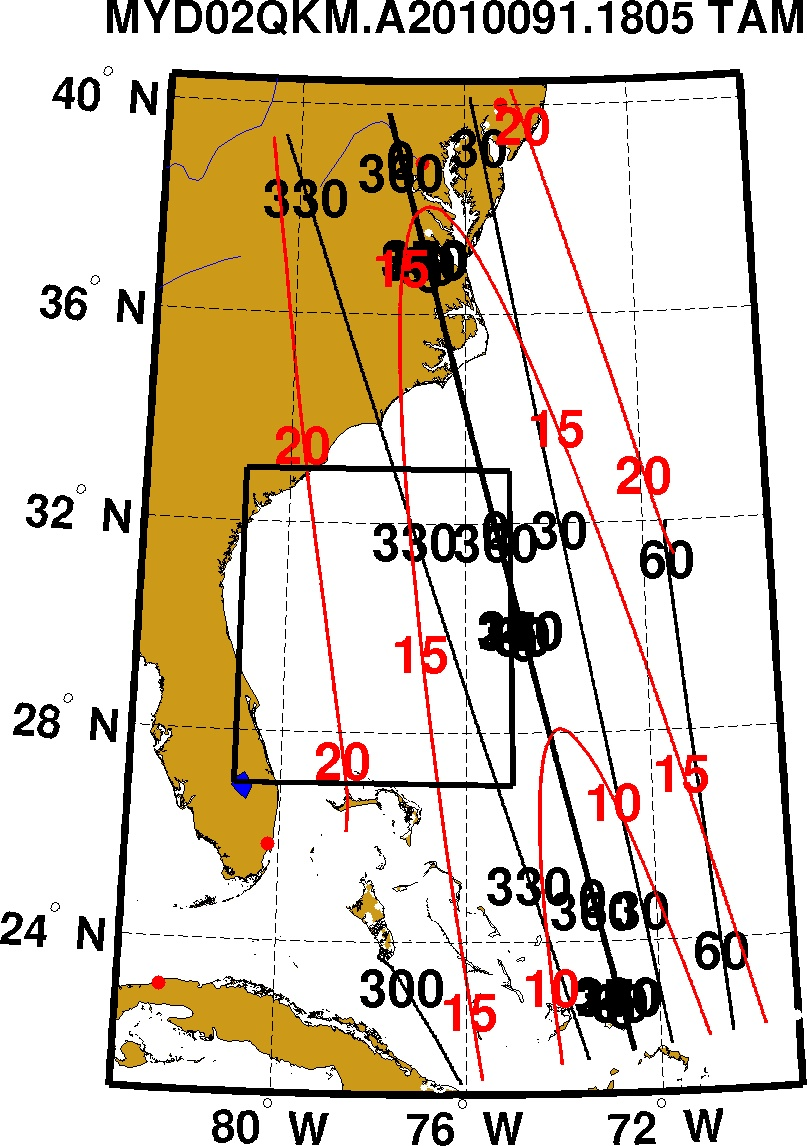
\includegraphics[width=1\linewidth]{fig17c}}
	\end{minipage}
	\\
    \floattitle{MERIS (а), MODIS/Terra (б) и MODIS/Aqua (в).
    \\
    Красные линии -- зенитный угол, чёрные -- азимут на Солнце}
    \caption{Карты локальных наклонов поверхности, обеспечивающие зеркальное отражение и , обусловленные геометрией наблюдений и положением солнца}
    \label{fig:17}
\end{figure}


Карты локальных наклонов поверхности характеризуют геометрию отражения/наблюдения, т.е. геометрию солнечного блика. Например при угле тильтирования (красные линии) 0${}^\circ{}$ образуется центральная зеркальная точка, а при возрастании этого угла, блик ``расплывается''. Азимут (чёрные линии) отвечает за форму эллипса блика, так, например, блик больше всего вытянут в направлении 0${}^\circ{}$ или 360${}^\circ{}$ и 180${}^\circ{}$.

По приведённым на Рисунке~\ref{fig:18} картам зон инверсии контрастов, можно отследить изменение зон инверсии контрастов при различных ветрах (цветные изолинии на Рисунке~\ref{fig:18}). Для данного примера были выбраны скорости ветра 3, 7, 11 и 15м/c, а также скорость ветра, построенная по данным NCEP GFS. При подробном рассмотрении этих изображений можно сделать вывод о том, что область нашего исследования находится вне зоны инверсии контрастов. Рассмотрение поведения передаточной функции непосредственно в зоне инверсии контрастов и объяснение причин их возникновения подробно приводится в Главе~\ref{chap:2}

На Рисунке~\ref{fig:17b} и Рисунке~\ref{fig:18b} приводятся карты локальных наклонов поверхности и положения зон инверсии контрастов для изображения MODIS/Terra, соответственно. Фрагмент изображения покрывает б\'{о}льшую часть Мексиканского залива, чтобы показать насколько далеко от центра блика находится область исследования.



\begin{figure}[!thb]
    	\centering
	\begin{minipage}{.33\textwidth}
	    \subcaptionbox{\label{fig:18a}}
		{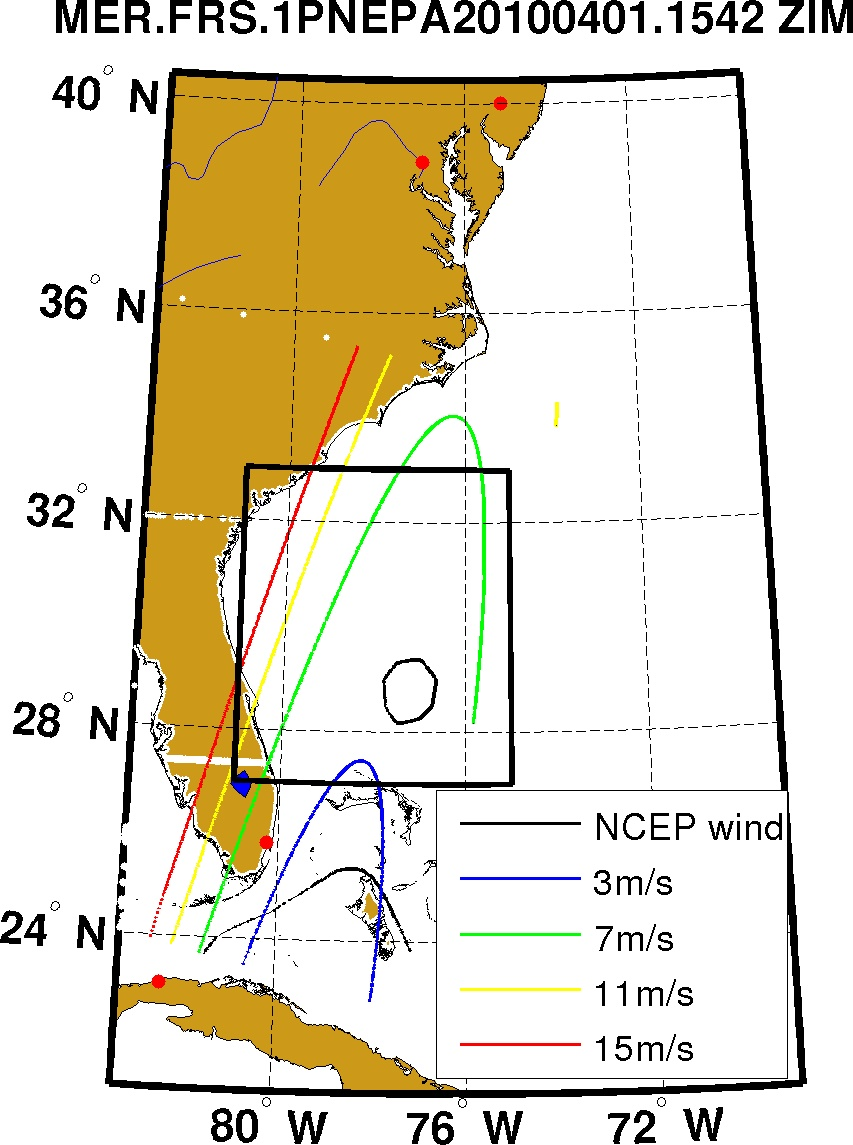
\includegraphics[width=1\linewidth]{fig18a}}
	\end{minipage}
	\hfill
	\begin{minipage}{.31\textwidth}
	    \subcaptionbox{\label{fig:18b}}
		{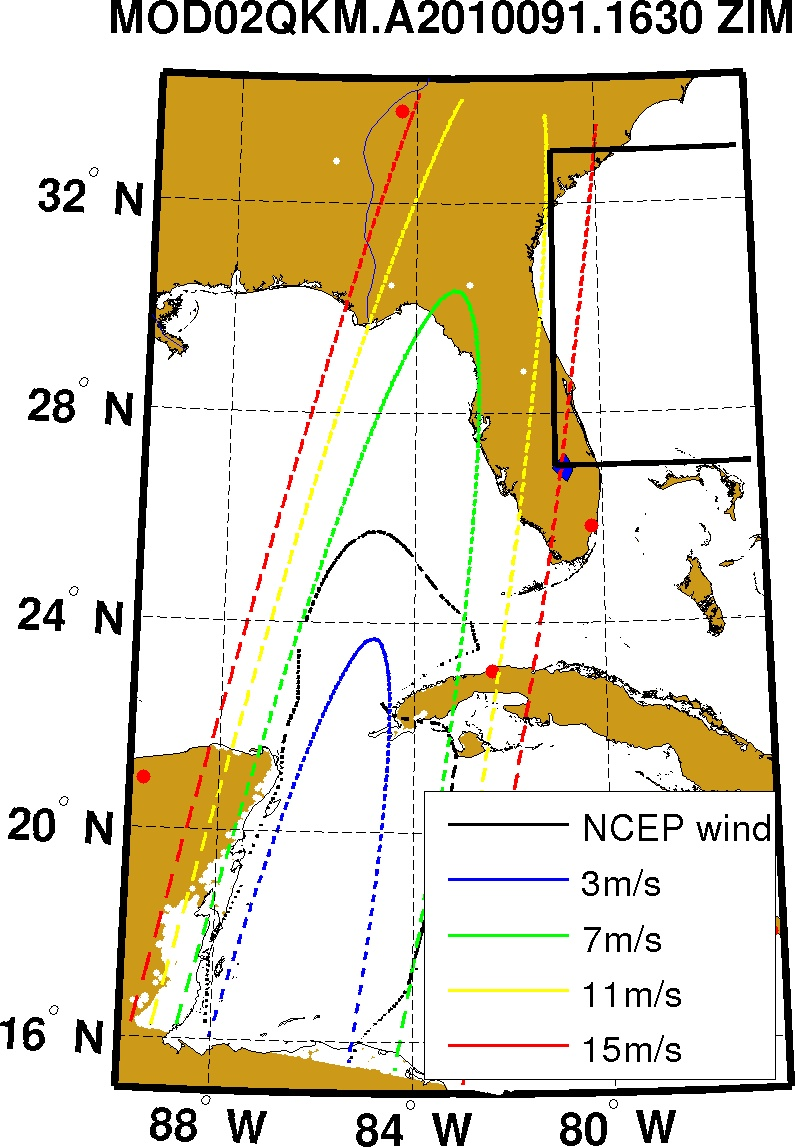
\includegraphics[width=1\linewidth]{fig18b}}
	\end{minipage}
	\hfill
	\begin{minipage}{.31\textwidth}
	    \subcaptionbox{\label{fig:18c}}
		{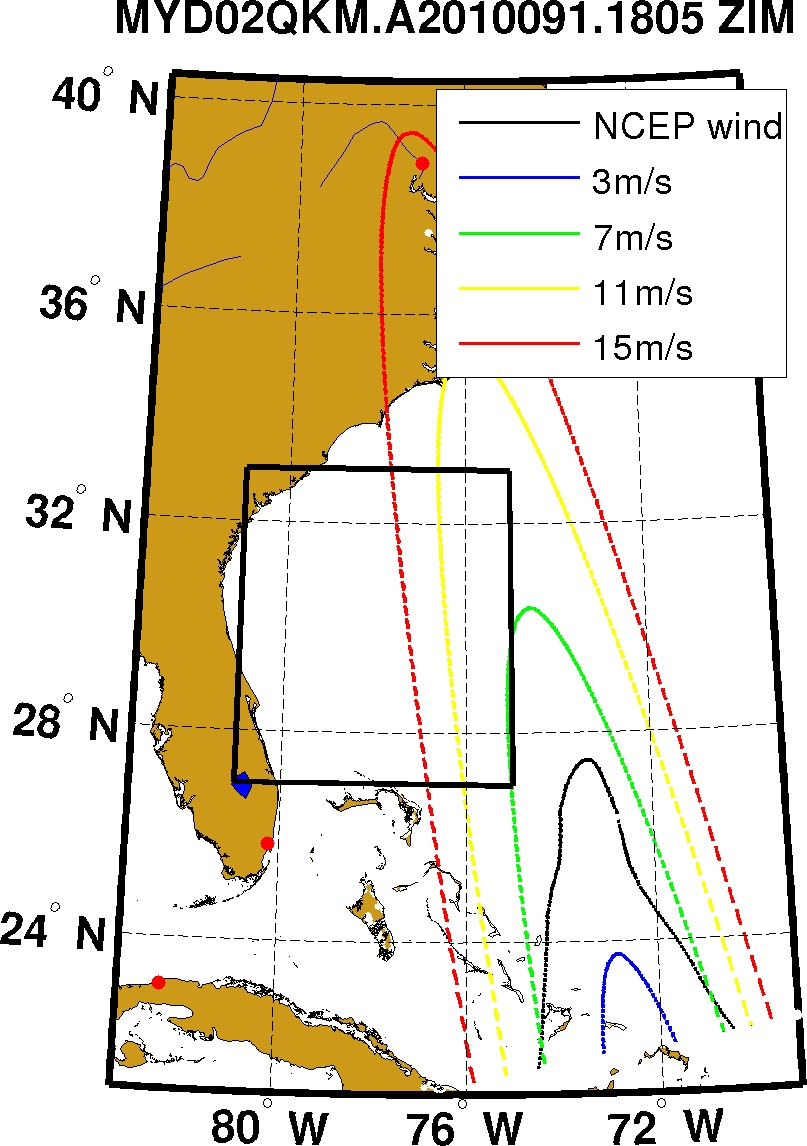
\includegraphics[width=1\linewidth]{fig18c}}
	\end{minipage}
	\\
    \floattitle{MERIS (а), MODIS/Terra (б) и MODIS/Aqua (в).
    \\
    Чёрная кривая - зона инверсии контрастов, рассчитанная для скорости ветра по модели NCEP, синяя, зелёная, жёлтая и красная - для 3, 7, 11 и 15м/с, соответственно}
    \caption{Карты зон инверсии контрастов для различных скоростей ветра}
    \label{fig:18}
\end{figure}


Расчёт карт локальных наклонов поверхности проводился, исходя из уравнения \eqref{eq:1.4}, используя формулы для расчёта уклонов \eqref{eq:1.3}. Карты зон инверсии контрастов находятся из решения урвнений \eqref{eq:1.7}, \eqref{eq:1.15}, в которых передаточная функция равна 0.

Карты локальных наклонов поверхности и карты зон инверсии контрастов позволяют не только упростить анализ сложных изображений, но и значительно повысить достоверность и точность количественных оценок наблюдаемых явлений.

Если следовать вышеприведённым шагам выполнения программы, реализующей разработанный алгоритм, в итоге мы получим контрасты СКН, приведённые на Рисунке~\ref{fig:19}.



\begin{figure}[!thb]
    	\centering
	\begin{minipage}{.31\textwidth}
	    \subcaptionbox{\label{fig:19a}}
		{\includegraphics[width=1\linewidth]{fig19a}}
	\end{minipage}
	\hfill
	\begin{minipage}{.31\textwidth}
	    \subcaptionbox{\label{fig:19b}}
		{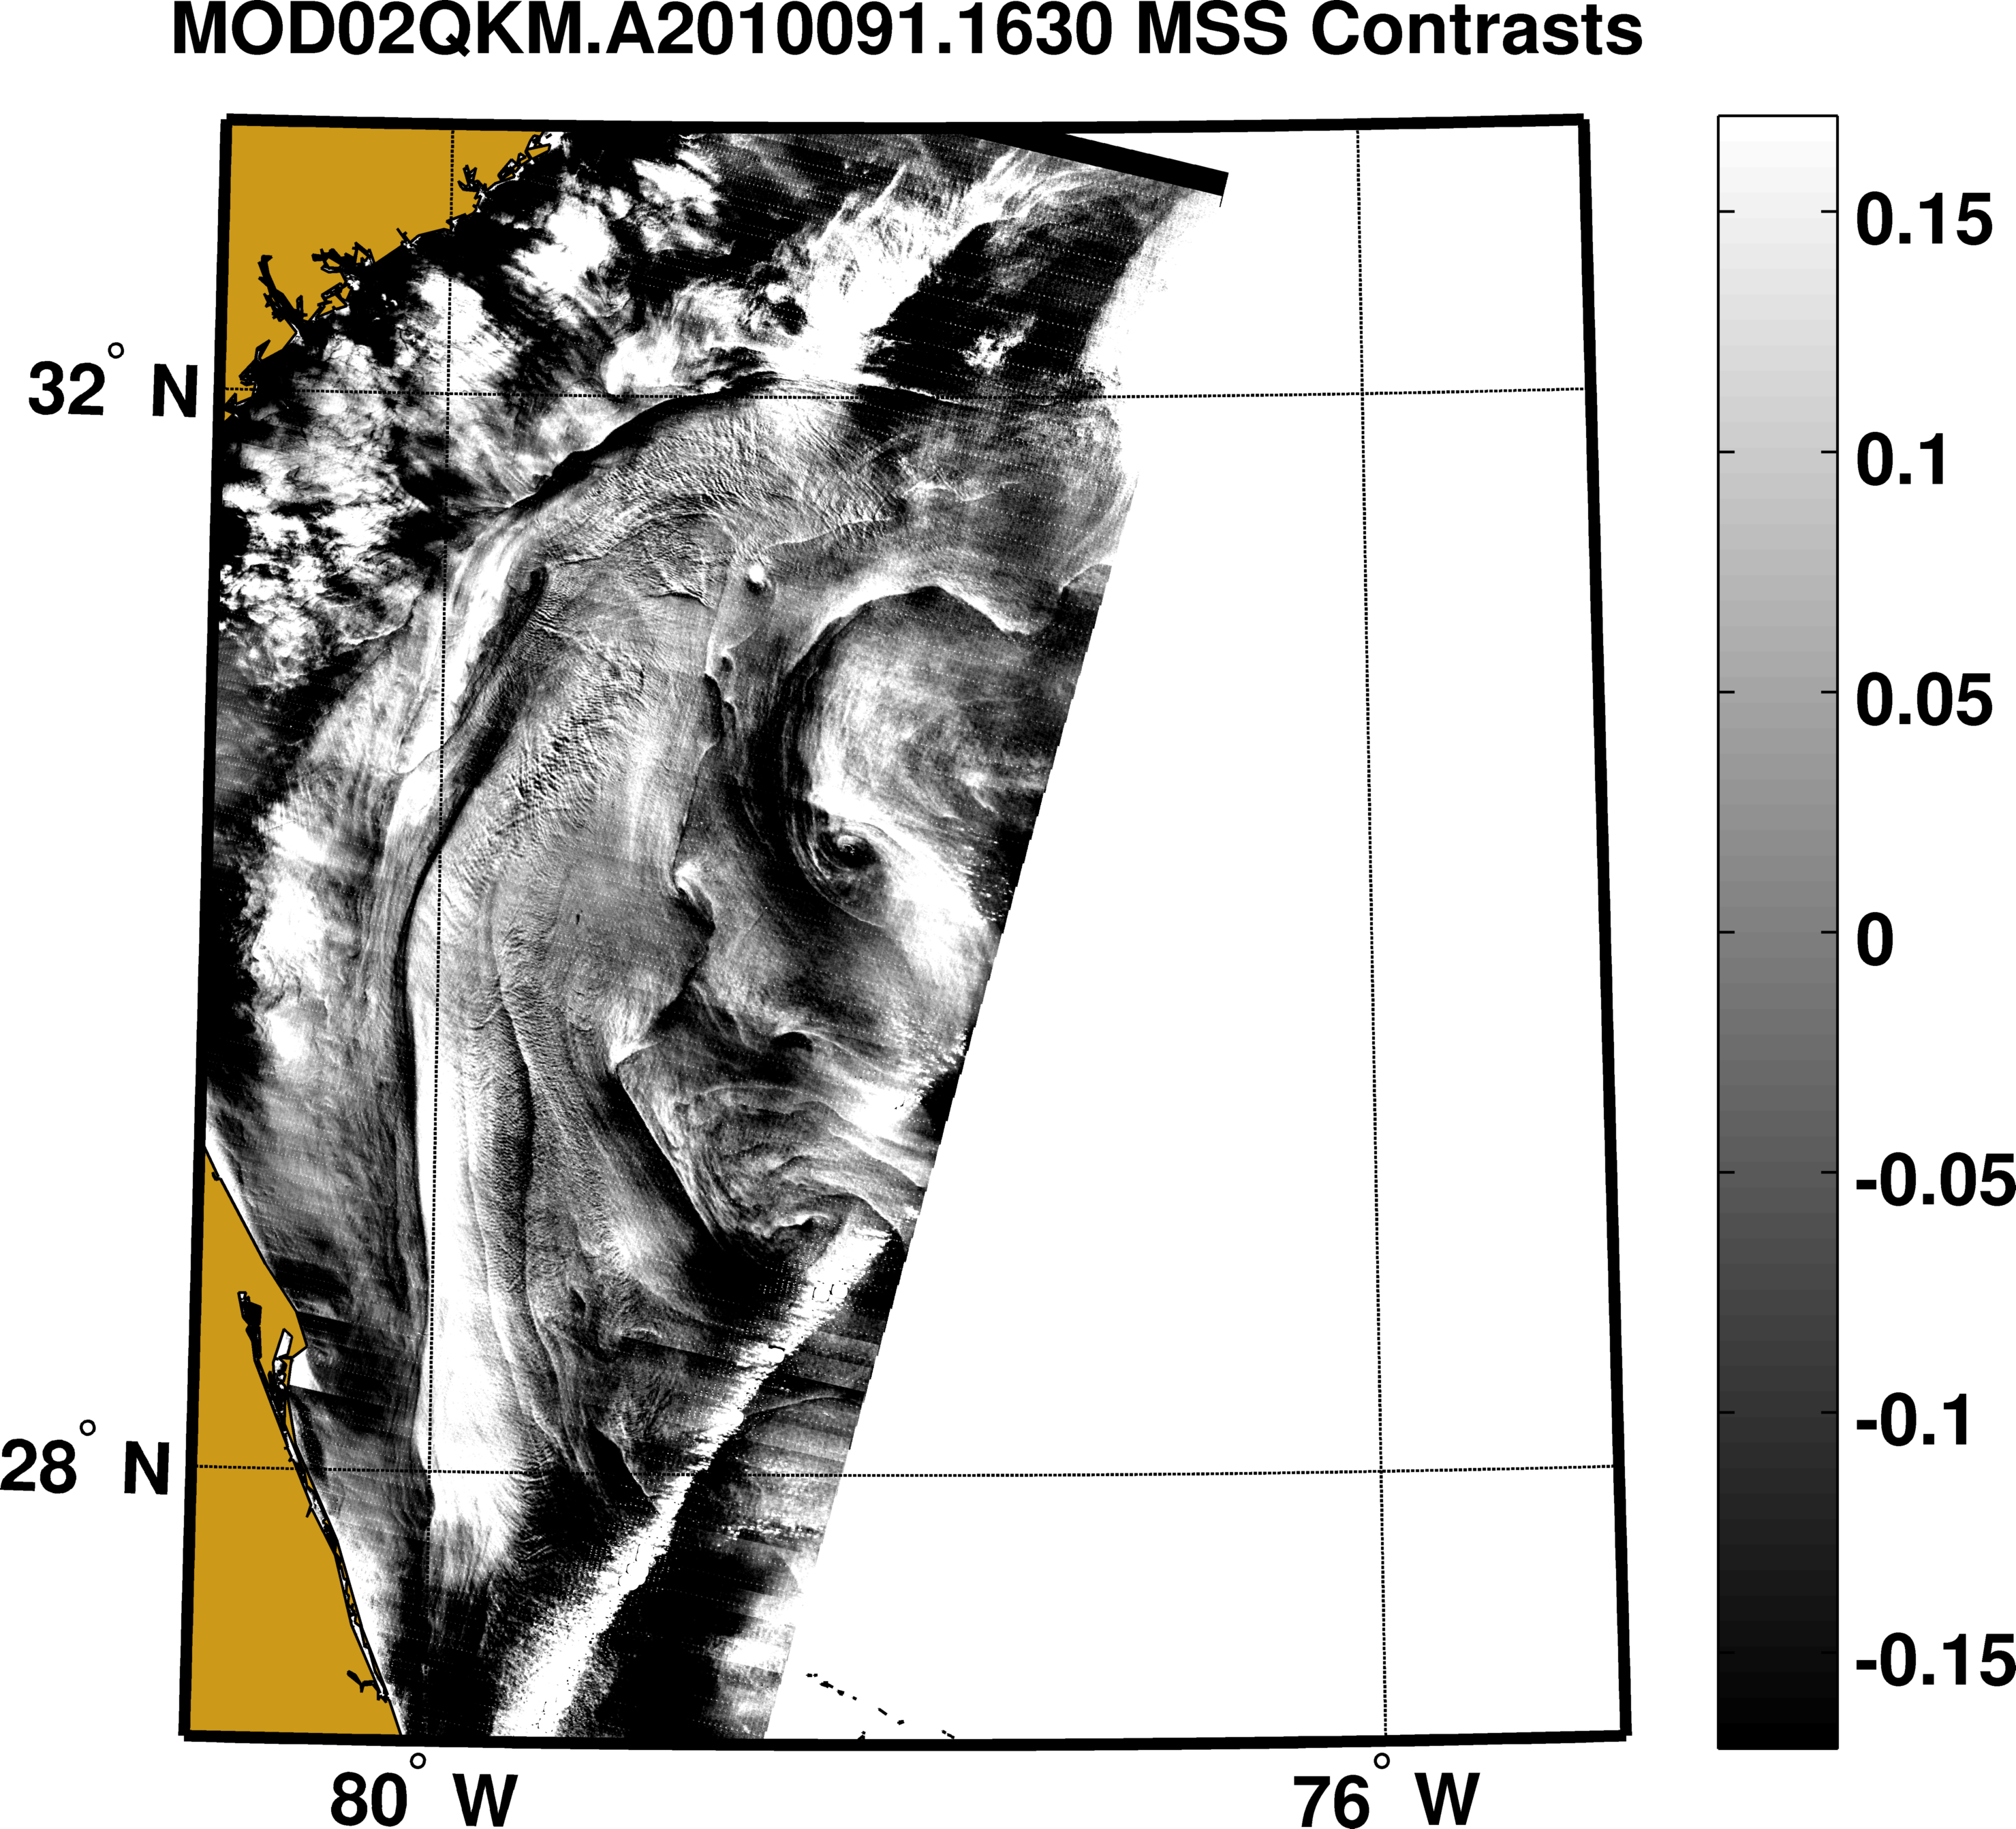
\includegraphics[width=1\linewidth]{fig19b}}
	\end{minipage}
	\hfill
	\begin{minipage}{.31\textwidth}
	    \subcaptionbox{\label{fig:19c}}
		{\includegraphics[width=1\linewidth]{fig19c}}
	\end{minipage}
	\\
    \floattitle{MERIS (а), MODIS/Terra (б) и MODIS/Aqua (в)}
    \caption{Контрасты СКН $\tilde{s}^{2} /s_{0}^{2} $}
    \label{fig:19}
\end{figure}


Рассмотрим ещё один любопытный пример. Возьмём сечения контрастов яркости $\tilde{B}/B_{0}$ изображений MODIS Terra и Aqua. На Рисунке~\ref{fig:20a} приведена увеличенная область с проведённым сечением по изображению MODIS Terra, представленного в полном масштабе на Рисунке~\ref{fig:15c},  а на Рисунке~\ref{fig:20b} --  MODIS Aqua. Сначала рассмотрим геометрию наблюдения данного района приборами MODIS, установленными на разных спутниках, в чём помогут рисунки с картами локальных наклонов поверхности. Первое, что стоит отметить, разность азимутальных углов наблюдения в районе сечения составляет около 100${}^\circ$, т.е. наблюдения приборами одной и той же области на поверхности Океана производятся практически под прямым углом. Во-вторых, угол тильтирования в районе сечения варьируется около 20${}^\circ$, а это значит, что мы находимся вне зоны инверсии контрастов, при скорости ветра около 3-5м/с.

На Рисунке~\ref{fig:20c} изображены сами сечения, взятые по изображениям MODIS Aqua (чёрная кривая) и Terra (красная кривая). Обращаю внимание читателей, что формы сечений очень похожи. Это является следствием того, что распределение уклонов морской поверхности азимутально практически изотропно ($\alpha =s_{c}^{2} /s_{u}^{2} =1$). А это, в соответствии с моделью формирования яркости морской поверхности Кокса и Манка~\citep{Cox1954}, приводит к точу, что наблюдаемые контрасты яркости и СКН не зависят от азимута наблюдений (относительно Солнца).



\begin{figure}[!h]
    	\centering
	\begin{minipage}{.47\textwidth}
	    \subcaptionbox{\label{fig:20a}}
		{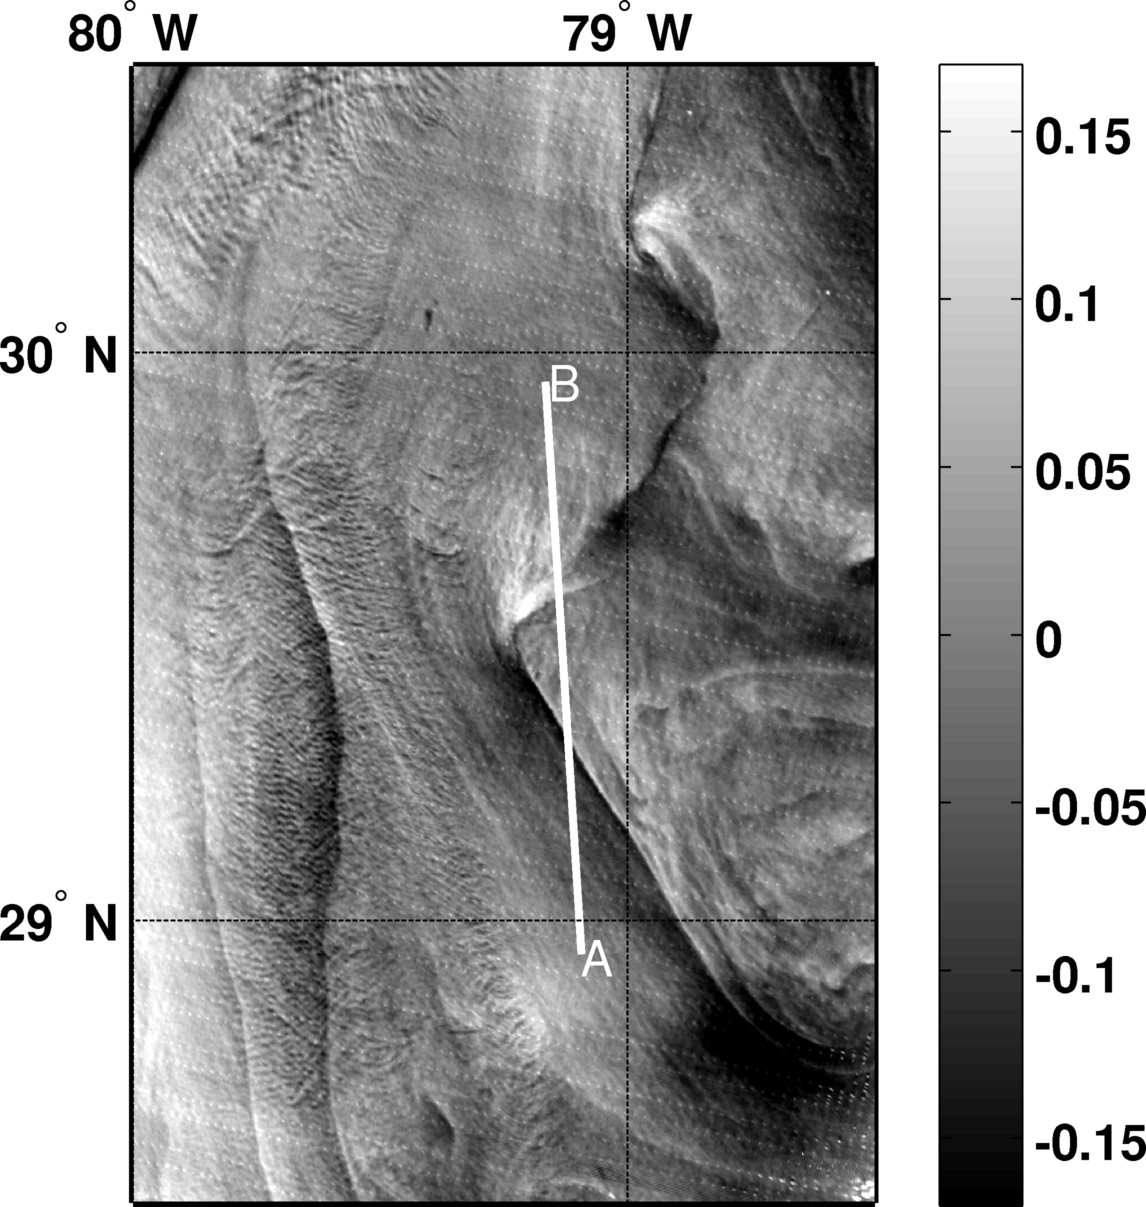
\includegraphics[width=1\linewidth]{fig20a}}
	\end{minipage}
	\hfill
	\begin{minipage}{.47\textwidth}
	    \subcaptionbox{\label{fig:20b}}
		{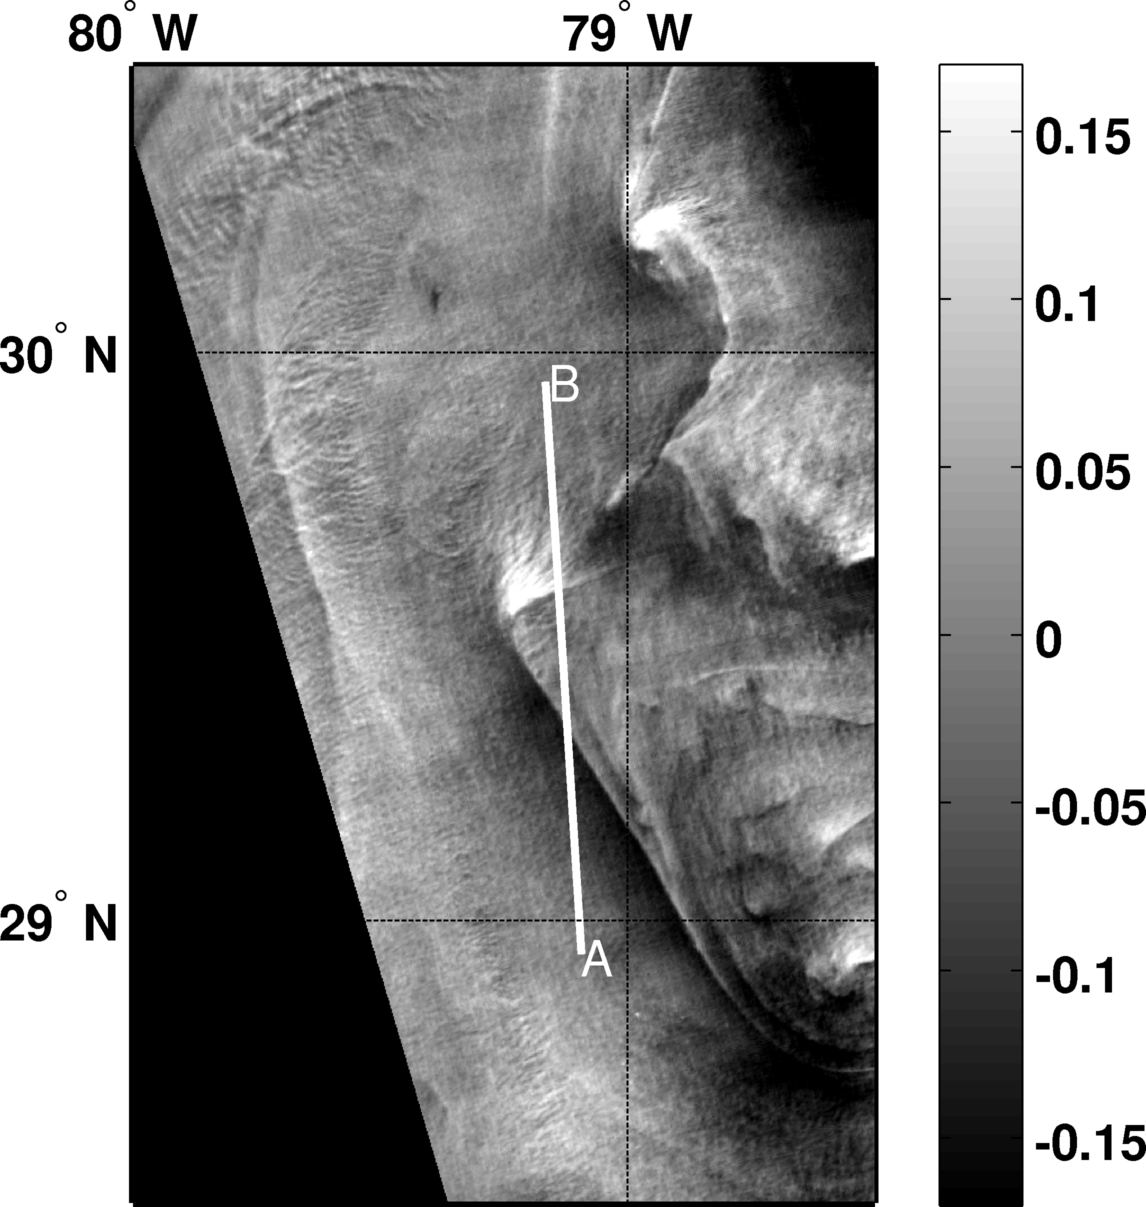
\includegraphics[width=1\linewidth]{fig20b}}
	\end{minipage}
	\hfill
	\\
	\begin{minipage}{.47\textwidth}
	    \subcaptionbox{\label{fig:20c}}
		{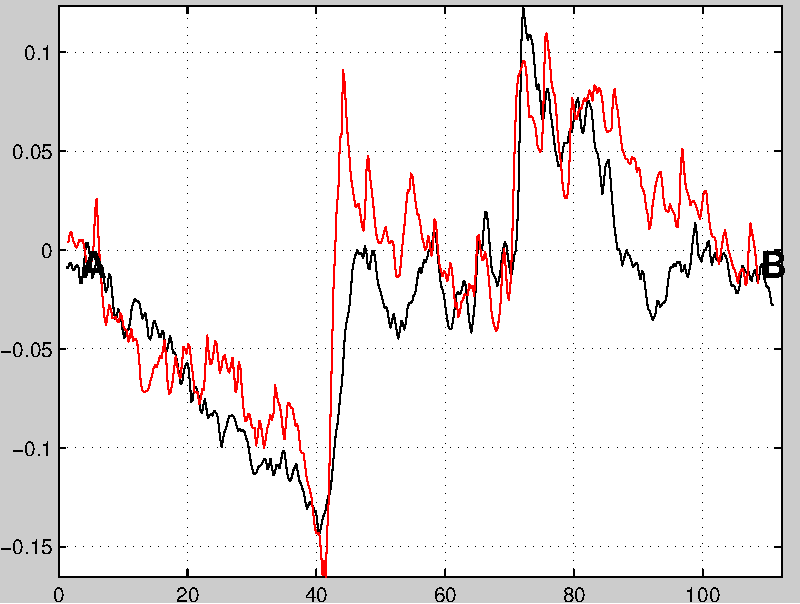
\includegraphics[width=1\linewidth]{fig20c}}
	\end{minipage}
	\\
    \floattitle{Изображения MODIS/Terra (а) и MODIS/Aqua (б) контрастов яркости с проведённым сечением (в)}
    \caption{Сечения контрастов яркости $\tilde{B}/B_{0}$}
    \label{fig:20}
\end{figure}


\newpage



\section{Выводы по главе}

В данной главе предложен метод восстановления пространственных вариаций среднеквадратичного наклона (СКН) морской поверхности по солнечному блику, регистрируемому оптическими сканерами из космоса. Вариации СКН могут быть связаны с поверхностными проявлениями различных процессов, происходящих в верхнем слое Океана, например, искусственными и биологическими сликами, внутренними волнами, градиентами мезо-масштабных течений и фронтальными разделами. С этой точки зрения, предложенный метод может рассматриваться как определенный шаг в направлении развития методов диагностики состояния поверхности Океана из Космоса.

Алгоритм восстановления основан на линейной связи вариаций яркости солнечного блика и контрастов СКН. Связь вариаций яркости солнечного блика и контрастов СКН осуществляется через передаточную функцию, которая зависит от пространственного распределения поля средней яркости солнечного блика.

При построении модели и разработки алгоритма предполагалось, что основной отклик морской поверхности на её возмущения, того или иного происхождения, вытекает из усиления, или же подавления СКН, в то время как другие статистические моменты, нормированные на СКН, изменяются незначительно. Это предположение основано на том факте, что несмотря на сильное подавление СКН в областях, покрытых сликами, коэффициенты анизотропии уклонов меняются незначительно \citep{Cox1956}.

Продемонстрировано, что при наличии 2-мерного поля яркости, передаточная функция может быть определена ``напрямую'' по усредненным градиентам яркости, непосредственно из 2D поля яркости солнечного блика без априорного задания какой либо модели плотности распределения вероятности (ПРВ) уклонов морской поверхности.

В тех случаях, когда 2-мерное поле яркости недоступно, передаточная функция определяется на основе априорного задании модели ПРВ.

Показано, что вариации яркости блика, вызванные одними и теми же явлениями, бывают как положительными, так и отрицательными. Область смены знака контраста яркости называется зоной инверсии контрастов. Происхождение этой зоны инверсии контрастов напрямую следует из определения модели формирования изображения солнечного блика. В этой зоне передаточная функция проходит через ноль, что приводит к сингулярному поведению восстановленных значений СКН в зоне инверсии контрастов.

Разработанный подход применим для любых спутниковых изображений в видимом диапазоне, в частности для данных, получаемых с оптических сканеров MODIS (Moderate Resolution Imaging Spectroradiometer) и MERIS (MEdium Resolution Imaging Spectrometer), которые широко используются для решения научных и прикладных задач.

В качестве дополнительного полезного ``продукта'' реализации предложенного метода восстановления СКН являются реконструированные вариации скорости ветра.

Определены границы применимости предложенного алгоритма, обусловленного геометрией наблюдений и положения солнца. Для чего построены карты локальных наклонов поверхности, а также карты зон инверсии контрастов.

Разработан комплекс программ, который позволяет производить:
\begin{itemize}
\item загрузку, чтение и обработку оптических (MODIS, MERIS) и радиолокационных (ASAR, RADARSAT-1,2) изображений, а также вспомогательных данных (например, о приводном ветре и маске Земли);
\item интерполировать геолокационные данные и данные о геометрии наблюдений;
\item маскирование облаков и земной поверхности, исключение ``битых'' пикселей;
\item устранение эффекта ``пилы'' и определение среднего и флуктуационного полей яркости;
\item восстановление СКН и приводной скорости ветра при помощи разработанного алгоритма, как с, так и без априорного задания плотности распределения уклонов;
\end{itemize}

Предложенные алгоритмы и методики реализованы и апробированы в Лаборатории Спутниковой Океанографии (ЛСО) РГГМУ, в виде элементов спутникового информационного портала SATIN (от англ. \textit{\textbf{SAT}}ellite Data Search and Manage \textit{\textbf{IN}}formation Portal), предназначенного для поиска, получения, отображения, распространения и хранения данных дистанционного зондирования (\url{http://satin.rshu.ru/}), а также как элемент разрабатываемой синергетической платформы SYNTool (\url{http://syntool.solab.rshu.ru/}) ЛСО РГГМУ.



\clearpage
